% GENERATED by paper/tools/accept_changes.py from paper/outline.tex (tracked changes accepted). Do not edit by hand.
% outline.tex -- writer's outline (8-page article). Build: tectonic outline.tex  (natbib plainnat, refs.bib)
\documentclass[10pt]{article}
\usepackage[margin=1.7cm]{geometry}
\usepackage{amsmath,amssymb}
\usepackage{enumitem}
\usepackage{multicol}
\usepackage[authoryear,round]{natbib}
\usepackage{url}
\usepackage{graphicx,booktabs,array}
\usepackage{needspace}% keeps supplementary headings with their text (Pass 18)
\usepackage{longtable}% Supplementary Table S6 (paper/supp/tableS6.tex)
\usepackage{changes}% tracked edits; use \usepackage[final]{changes} for clean text
\definechangesauthor[name={Pass 3}, color=teal]{P3}
\definechangesauthor[name={Pass 4}, color=purple]{P4}% sweep-only rescope of 2026-11-02; change log paper/pass4_changelog.md
\definechangesauthor[name={Pass 5}, color=orange]{P5}% replication across training seeds, added 2026-11-02; change log paper/pass5_changelog.md
\definechangesauthor[name={Pass 6}, color=brown]{P6}% hypervolume and share of non-dominated strengths, 2026-11-02; change log paper/pass6_changelog.md
\definechangesauthor[name={Pass 7}, color=violet]{P7}% sweep Results and Discussion; change log paper/pass7_changelog.md
\definechangesauthor[name={Pass 8}, color=magenta]{P8}% results-independent edits (update-step bullet moved to Methods, limitations, MMD kernel, Li et al. framing, hypervolume label, wording); change log paper/pass8_changelog.md
\definechangesauthor[name={Pass 9}, color=olive]{P9}% result placeholders filled from the sweep, the placement check and the biology check; Conclusions; change log paper/pass9_changelog.md, numbers in paper/pass9_numbers.csv
\definechangesauthor[name={Pass 11}, color=blue]{P11}% real Figure 1 (schematic and one real sweep example); change log paper/pass11_changelog.md, numbers in paper/pass11_numbers.csv
\definechangesauthor[name={Pass 10}, color=teal]{P10}
\definechangesauthor[name={Pass 14}, color=violet]{P14}% replication across training seeds filled in; change log paper/pass14_changelog.md, numbers in paper/pass14_numbers.csv
\definechangesauthor[name={Pass 15}, color=cyan]{P15}% re-review fixes and abstract cut; change log paper/pass15_changelog.md
\definechangesauthor[name={Pass 16}, color=green]{P16}% family-level sign-flip sensitivity analysis; change log paper/pass16_changelog.md, numbers in paper/pass16_numbers.csv
\definechangesauthor[name={Pass 17}, color=olive]{P17}% finished supplement placed in the list, main-text corrections; change log paper/pass17_changelog.md, numbers in paper/pass17_numbers.csv
\definechangesauthor[name={Pass 19}, color=blue]{P19}% AI-tool statement in Methods; change log paper/pass19_changelog.md
\definechangesauthor[name={Pass 20}, color=blue]{P20}% Declarations: ethics wording, competing interests; change log paper/pass20_changelog.md
\definechangesauthor[name={Pass 23}, color=blue]{P23}% Results walkthrough decisions; change log paper/pass23_changelog.md
\definechangesauthor[name={Pass 22}, color=red]{P22}% cut wordiness, content kept; change log paper/pass22_changelog.md
\definechangesauthor[name={Pass 13}, color=orange]{P13}% abstract cut, consecutive table numbers, reference-batch justification; change log paper/pass13_changelog.md, numbers in paper/pass13_numbers.csv
\definechangesauthor[name={Pass 12}, color=red]{P12}% rigour-review fixes; change log paper/pass12_changelog.md, numbers in paper/pass12_numbers.csv (checked by paper/tools/check_ledger.py)% real Figures 2-6, \tbd items answered from repository records; change log paper/pass10_changelog.md, numbers in paper/pass10_numbers.csv
\usepackage{todonotes}
% Pass 8: a bullet removed as a tracked deletion; nothing (no empty bullet) in the [final] build
\makeatletter
\newcommand{\droppeditem}[1]{\@ifpackagewith{changes}{final}{}{\item \deleted[id=P8]{#1}}}
\makeatother
\usepackage[hidelinks]{hyperref}
\setlist{nosep,leftmargin=1.2em,topsep=0pt,itemsep=0pt}
\setlength{\emergencystretch}{3em}
\setlength{\parindent}{0pt}
\setlength{\parskip}{0pt}
\renewcommand{\bibfont}{\scriptsize}
\setlength{\bibsep}{0pt}
\newcommand{\pp}[2]{\par\vspace{3pt}\noindent\textbf{#1.}\ #2\par\nopagebreak}
\newcommand{\res}[1]{[\textit{result: #1}]}
\newcommand{\tbd}[1]{[\textit{to be decided: #1}]}
\newcommand{\hd}[2]{\section*{#1 \hfill {\normalfont\small #2}}\vspace{-4pt}}

\begin{document}
\begin{center}
{\large\bfseries Benchmarking alignment penalties for single-cell batch correction}\\[2pt]
{\small Kendall Reid$^{1,*}$, Genevieve Stein-O'Brien$^{2,\dagger}$, Erhan Guven$^{3,\dagger}$}\\[1pt]
{\footnotesize $^1$Department of Computer Science, Johns Hopkins University; $^2$Department of Neuroscience, Johns Hopkins University; $^3$Johns Hopkins University Applied Physics Laboratory. $^*$Corresponding author: kreid20@jh.edu. $^\dagger$These authors contributed equally.}\\[1pt]
{\footnotesize }
\end{center}
{\footnotesize \textbf{Writer's outline.} Target: \emph{BMC Bioinformatics}, Research article; structured abstract at most 350 words; 3 to 10 keywords; no stated word, figure or reference limit; Declarations required; large language model use documented in Methods. Main text about 5,000 words plus 400 words of captions; paragraphs 100--150 words. Brackets: fill from results or still open. Background and Methods are the first author's prose with tracked corrections (\texttt{changes} package; change logs in \texttt{paper/drafts\_20261022/}, \texttt{paper/drafts\_20261023\_pass3/} and \texttt{paper/pass4\_changelog.md}. Pass 4 reframes the draft around the finished penalty-strength sweep: the benchmark at fixed strengths is not run, by the first author's decision of 2 November 2026; Pass 5 adds the replication across training seeds that replaced that benchmark, decided by the first author on the same day (change log \texttt{paper/pass5\_changelog.md})). Figures 1--6 are drawn from the sweep analysis (Figures 2--6 in Pass 10, Figure 1 in Pass 11, \texttt{paper/figure\_scripts}, change logs \texttt{paper/pass10\_changelog.md} and \texttt{paper/pass11\_changelog.md}); Tables \ref{tab:3} and \ref{tab:4} hold sweep values (Pass 9, change log \texttt{paper/pass9\_changelog.md}, number ledger \texttt{paper/pass9\_numbers.csv}); In Pass 23 Figure 4, the Pareto frontier, was added, and the local-versus-global analysis (panel c of the former Figure 4) and the good-strength width (the former Figure 5) were removed, so Figures 1--6 are drawn from the sweep analysis. Table \ref{tab:1} holds real design facts; the strength-range table of the planned fixed-strength benchmark, which is not run, was removed in Pass 4. Pass 13 numbered the main-text tables 1 to 3 (the methods, the ranking and the placement table; since Pass 23 they are Supplementary Tables \ref{tab:1}, \ref{tab:3} and \ref{tab:4}) and every reference to them is made by label. Pass 12 (change log \texttt{paper/pass12\_changelog.md}) fixes the points of the Pass 11 rigour review; every abstract number is listed with its source in \texttt{paper/pass12\_numbers.csv} and re-read by \texttt{paper/tools/check\_ledger.py}. Pass 14 fills the replication across training seeds from its result (change log \texttt{paper/pass14\_changelog.md}, numbers in \texttt{paper/pass14\_numbers.csv}, Supplementary Table S9 generated by \texttt{paper/tools/make\_replication.py}). Pass 15 fixes the points of the independent re-review and cuts the abstract (change log \texttt{paper/pass15\_changelog.md}); the clean copy \texttt{paper/outline\_clean.tex} is written by \texttt{paper/tools/accept\_changes.py}. Pass 16 adds the family-level sign-flip sensitivity analysis to the replication result (change log \texttt{paper/pass16\_changelog.md}). Pass 17 places the finished supplement (Supplementary Notes 2--12, Tables S1, S2, S4, S5 and S8) in the supplementary list and corrects the main text where the supplement's sources showed it wrong (change log \texttt{paper/pass17\_changelog.md}).}

\hd{Abstract}{at most 350 words; Background, Results, Conclusions}
\begin{enumerate}[leftmargin=1.5em]
\item \textbf{Background:} Single-cell batch correction often adds an alignment penalty (a discriminator, a Wasserstein-1 critic or a distance between batches) to a generative model, but penalties have rarely been compared on one backbone.
\item Question: which penalty keeps the most biology at equal batch removal in one scVI (single-cell variational inference) model, and does any beat plain scVI or standard tools?
\item Exploratory comparison on eight tasks of the single-cell integration benchmark: scVI plus the Jensen--Shannon discriminator, three Wasserstein-1 critics (reference, pooled, barycenter), maximum mean discrepancy (MMD) or the Sinkhorn divergence, each fitted at ten strengths from 0.1 to 3,000, with the decoder given the batch label or not and three seeds (100--102), beside plain scVI and standard tools. Instead of a planned fixed-strength run, the two sweep strengths bracketing matched batch removal were refitted with five new seeds (0--4).
\item \textbf{Results:} The pooled critic had the best mean rank with the batch-conditioned decoder (2.20 over five real tasks), and MMD with the unconditioned decoder (2.17 over six real tasks).
\item Up to the highest common batch score, collapse rates with the batch-conditioned decoder peaked at 10\% (1\%--30\%) for MMD and 56\% (31\%--78\%) for the discriminator (nominal 95\% intervals).
\item With this decoder, a penalty at one strength drawn at random exceeded plain scVI's selection score on at most 3 of six real tasks, and the best of six strengths on 4 to 6; at six tries every penalty exceeded Harmony and sysVI on 5 of six real tasks.
\item A replication across training seeds kept the sign of all four large within-pair differences (mean rank correlation 0.456, $p=0.00049$), but on new seeds the Sinkhorn divergence and the pooled critic led, and the discriminator stayed last with the batch-conditioned decoder.
\item \textbf{Conclusions:} Within these tasks, strength mattered more than penalty choice: penalties were near-tied at matched batch removal (160 of 195 within-pair differences under 0.02); a penalty exceeded batch-conditioned plain scVI mainly when several strengths were tried and scored on the same data, an optimistic gain; scANVI, trained with the cell-type labels that several biology metrics also use, exceeded every penalty on most tasks. Code and checksums: github.com/kreid415/wasserstein-critic-deconfounding.
\end{enumerate}
\par\vspace{3pt}\noindent\textbf{Keywords:} single-cell RNA sequencing; batch correction; adversarial learning; optimal transport; benchmarking

\section[Background]{Background}
% intro_tracked.tex -- Introduction of USER_DRAFT with tracked corrections.
% Markup: LaTeX `changes' package (\added{new}, \deleted{old}, \replaced{new}{old}).
% Preamble needed by the integrating document:  \usepackage[authoryear,round]{natbib}  \usepackage{changes}
%   (build with \usepackage[final]{changes} to print the corrected text only).
% \protect precedes \citep inside \deleted{} so that the strike-out markup does not break the citation.
% Change log with sources: intro_changelog.md. Bibliography: paper/refs.bib (no new entries needed).
% Base text: brief/user_draft.tex lines 42-54 (Introduction), checked against paper/outline.tex Intro-1..8 (commit 8c89960).

\qquad Single-cell RNA-seq captures each cell's transcriptional state at one time point, but biological differences in a dataset can be masked by technical differences between  samples. Laboratory conditions, reagent lots, personnel and instruments introduce technical variation, which becomes a confounder when it is correlated with the biological outcome \citep{leek2010tackling,yu2024assessing}. Separately processed technical replicates of single-cell RNA-seq can differ substantially \citep{tung2017batch}, and single-cell data pose new problems for modelling batch effects \citep{goh2022batch}. Batch correction methods include Harmony \citep{korsunsky2019fast}, Scanorama \citep{hie2019efficient}, scVI (single-cell variational inference) \citep{lopez2018deep}, its label-aware extension scANVI \citep{xu2021probabilistic} and sysVI \citep{hrovatin2025integrating}. Each must balance the alignment of batches against the preservation of biological signal \citep{luecken2022benchmarking}: under-correction leaves substantial batch effects, and over-correction discards key biological information \citep{yu2024assessing}.

\qquad Deep-learning methods for single-cell analysis need batch correction that is trained end to end with the model. Latent-variable models learn a low-dimensional representation of the RNA-seq readout that captures  biological programs. Two approaches align these latent spaces across batches: decoder conditioning, which passes the batch label  to the decoder that reconstructs the input RNA-seq vector from the latent variable \citep{lopez2018deep}, and adversarial training, which trains a network to predict the batch, or another confounder such as age, from each cell's latent code and penalizes the encoder whenever that prediction succeeds \citep{ganin2016domain,dincer2020adversarial}.

\qquad Adversarial methods use either a discriminator, which minimizes the Jensen--Shannon (JS) divergence \citep{goodfellow2014generative} between samples from different batches or confounder values \citep{ganin2016domain,dincer2020adversarial}, or a Wasserstein critic, which minimizes the Wasserstein-1 (W1) distance \citep{arjovsky2017wasserstein,gulrajani2017improved} between such samples. Both have been applied widely to single-cell batch correction.

\qquad iMAP trained a critic with the gradient penalty of the Wasserstein generative adversarial network (WGAN-GP) and corrected every dataset towards one anchor dataset that is left unchanged \citep{wang2021imap}. iDLC trains a WGAN-GP critic, with a Sinkhorn transport term in the generator loss, to map each source batch onto a reference batch \citep{jiang2026geometric}; scStarCorrect also aligns every batch to one fixed reference batch,  through a domain-aware discriminator whose loss form its abstract does not state \citep{gu2025scstarcorrect}; Beaconet trains one Wasserstein critic per batch against the mixture of the other batches and needs no reference \citep{xu2024beaconet}. IMGG trains a WGAN-GP generator towards a synthetic intermediate batch built from cells matched across batches \citep{wang2022imgg}, ResPAN combines a Wasserstein GAN with random-walk mutual-nearest-neighbour pairing \citep{wang2022respan}, and IMAAE uses a WGAN-GP-form loss, an anchor batch and known cell labels \citep{wang2023integrating}. Discriminator-based methods are also common. Portal trains two logistic discriminators and clamps their logits so that cells scored as clearly dataset-specific give no gradient and are not forced to mix \citep{zhao2022adversarial}; AIF pairs a real-versus-reconstructed discriminator with a batch classifier that the encoder is trained against \citep{monnier2024novel}; and ABC trains an autoencoder against a multi-class batch discriminator alongside cell-type classifier branches that use labels \citep{danino2024batch}.

\qquad A third route measures the distance between the latent batches directly, with no adversary network: the maximum mean discrepancy (MMD) \citep{gretton2012kernel} and optimal transport (OT) measures \citep{cuturi2013sinkhorn, genevay2018learning,feydy2019interpolating} (formulations in Supplementary Note 1). Both  have been used to align single-cell batches. MMD-ResNet trains a residual network to match the distribution of one batch to that of another \citep{shaham2017removal}, SAUCIE applies an MMD penalty against a reference batch on an internal layer \citep{amodio2019exploring}, trVAE places an MMD term across conditions in the first decoder layer \citep{lotfollahi2020conditional}, uniPort couples a variational autoencoder with minibatch unbalanced OT \citep{cao2022unified}, and Li et al.\ added an MMD term between batches to the loss of an early scVI version \citep{li2022trade}.

\qquad Alignment penalties have limitations that challenge their utility in practice. When batches contain different cell-type proportions, a lower bound on classification error grows as the latent distributions of the two batches are aligned more tightly \citep{zhao2019learning}, and exact alignment under any divergence that is zero only for identical distributions leaves an error at least as large as the proportion gap \citep{wu2019domain}. The sysVI study found that an adversarial conditional variational autoencoder and an adversarial multi-omics integration method mixed unrelated cell types when proportions were unbalanced across batches,  more so at higher adversarial strength \citep{hrovatin2025integrating}; dataset imbalance also changed clustering, annotation, differential expression, query mapping and trajectories across five integration methods \citep{maan2024characterizing}.

% This section below should be a short sentence of two before the result

% \added{Image-GAN studies caution against attributing a difference to the divergence alone. With enough hyperparameter search and random restarts, most GAN losses reached similar scores, and none consistently beat the original non-saturating loss \citep{lucic2018gans}; that loss was stable across datasets, spectral normalisation helped consistently, and the gradient penalty helped only sometimes \citep{kurach2019large}. A difference between a critic and a discriminator may therefore come from regularisation, the number of adversary updates or tuning rather than from the divergence. These are image results; our follow-up experiment tests whether they carry over, by varying the regulariser and the update steps while holding the backbone fixed.}


\qquad Large benchmarks have compared batch-correction methods \citep{tran2020benchmark,luecken2022benchmarking,luecken2025defining}, but each method brings its own architecture, preprocessing and training settings, so these benchmarks cannot show which alignment objective accounts for a method's performance. Controlled comparisons of alignment losses inside one framework are few. The extended single-cell integration benchmark (scIB-E) compared six batch losses, one of them a GAN discriminator, inside one scVI framework, with no Wasserstein, MMD or OT term \citep{yi2025benchmarking}; Li et al.\ compared MMD with an adversarially trained mutual-information penalty on an early scVI version and traced the Pareto front between batch removal and biology \citep{li2022trade}; and the iDLC ablation removes its Sinkhorn term but has no JS or MMD arm \citep{jiang2026geometric}. In searches of OpenAlex, arXiv and Europe PMC run in October 2026 and repeated in OpenAlex and Europe PMC on 5 November 2026 for works published since 1 October 2026, we found no study that compares JS, W1 and MMD or OT objectives on one stock scVI backbone; this absence rests on those searches and is  not exhaustive.



\qquad We benchmark discriminator-, critic-, kernel- and optimal transport-based alignment penalties for batch correction: the JS discriminator, three variants of the Wasserstein critic (reference, pooled and barycenter), MMD and the Sinkhorn divergence, compared with standard baselines. Each penalty is added to the same scVI model \citep{lopez2018deep}, with the decoder either given the batch label or not, and evaluated on eight tasks of the single-cell integration benchmark scIB \citep{luecken2022benchmarking}. Backbone, tasks and  training settings are fixed except the adversary update steps and optimiser, which follow each method's usual setting, so differences between methods come from the alignment penalty as it is usually run. The comparison is exploratory: every penalty is fitted across one strength range on every task, and the analysis reads all of those fits. A benchmark at fixed strengths, planned to follow the sweep, was replaced by a smaller replication across training seeds: at the two sweep strengths on either side of the batch removal at which the penalties are compared (Methods), each penalty is refitted with five new seeds (0--4) on the same eight tasks, and the new fits are compared with the sweep's readings by a rule fixed before any of them was scored. The replication uses new seeds, not new data. It shows whether the sweep's readings hold when the training seed changes; its rule tests only the sign of  within-pair differences of 0.04 or more (no precision calculation was made), so it does not test the order of penalties that sit close together.

% this should be in methods
% We compare all of these approaches with plain scVI and with Harmony \citep{korsunsky2019fast}, Scanorama \citep{hie2019efficient}, scANVI \citep{xu2021probabilistic} and sysVI \citep{hrovatin2025integrating} at equal numbers of tries, allowing for the outcome that no alignment penalty improves on plain scVI.
% A stronger penalty trades biology for batch removal along a curve, as Li et al.\ showed for scVI \citep{li2022trade}. We therefore read each method's biology score where all methods reach the same batch removal. For each penalty we also report how often it collapses and how narrow its range of good strengths is.
% DONE: moved to Methods (matched-batch-removal, baselines and secondary-analysis paragraphs)


\section{Methods}
% methods_tracked.tex -- Methods of USER_DRAFT with tracked corrections (LaTeX `changes` package:
% \added{}, \deleted{}, \replaced{new}{old}). Preamble needs \usepackage{changes} and the \tbd macro of outline.tex.
% Change numbers (C1, C2, ...) refer to methods_changelog.md. \todo commands of the draft are removed; their text is
% shown as \deleted{\textit{todo: ...}} so the deletion is visible.
% Written 2026-10-21 from the sources listed in methods_changelog.md. No main-benchmark or follow-up result was read.

% ---- Paragraph 1: backbone (user paragraph 1) ----
\qquad For a fair comparison all methods share one backbone, scVI (single-cell variational inference)  \citep{lopez2018deep}, implemented in the scvi-tools python package \citep{gayoso2022python}. Every method uses scvi-tools' default settings and likelihood, with epochs, minibatch size and latent size equal within a task, so that the alignment method and its strength are the only intended differences apart from the adversary update steps and their optimiser, which follow each method's  standard setting: the reference, pooled and barycenter critics take five update steps per encoder step with a gradient penalty, as is usual for Wasserstein critics \citep{gulrajani2017improved}, and the discriminator takes one update step, as is usual for discriminators, so the penalties are compared as they are normally run (Supplementary Note 2). We use two settings: a conditioned setting in which the batch label is fed to the decoder, as scVI is usually run, and an unconditioned setting in which no batch label reaches the encoder or decoder, so the alignment penalty is the only correction (Figure 1a). Hyperparameters and training details are  in Supplementary Table S2 and Supplementary Note 2.

% Pass 21: main figures placed in the text for editing (paper/pass21_changelog.md); journal layout later.
% ---------------------------------------------------------------- Figure 1
\begin{figure}[!htbp]
\centering
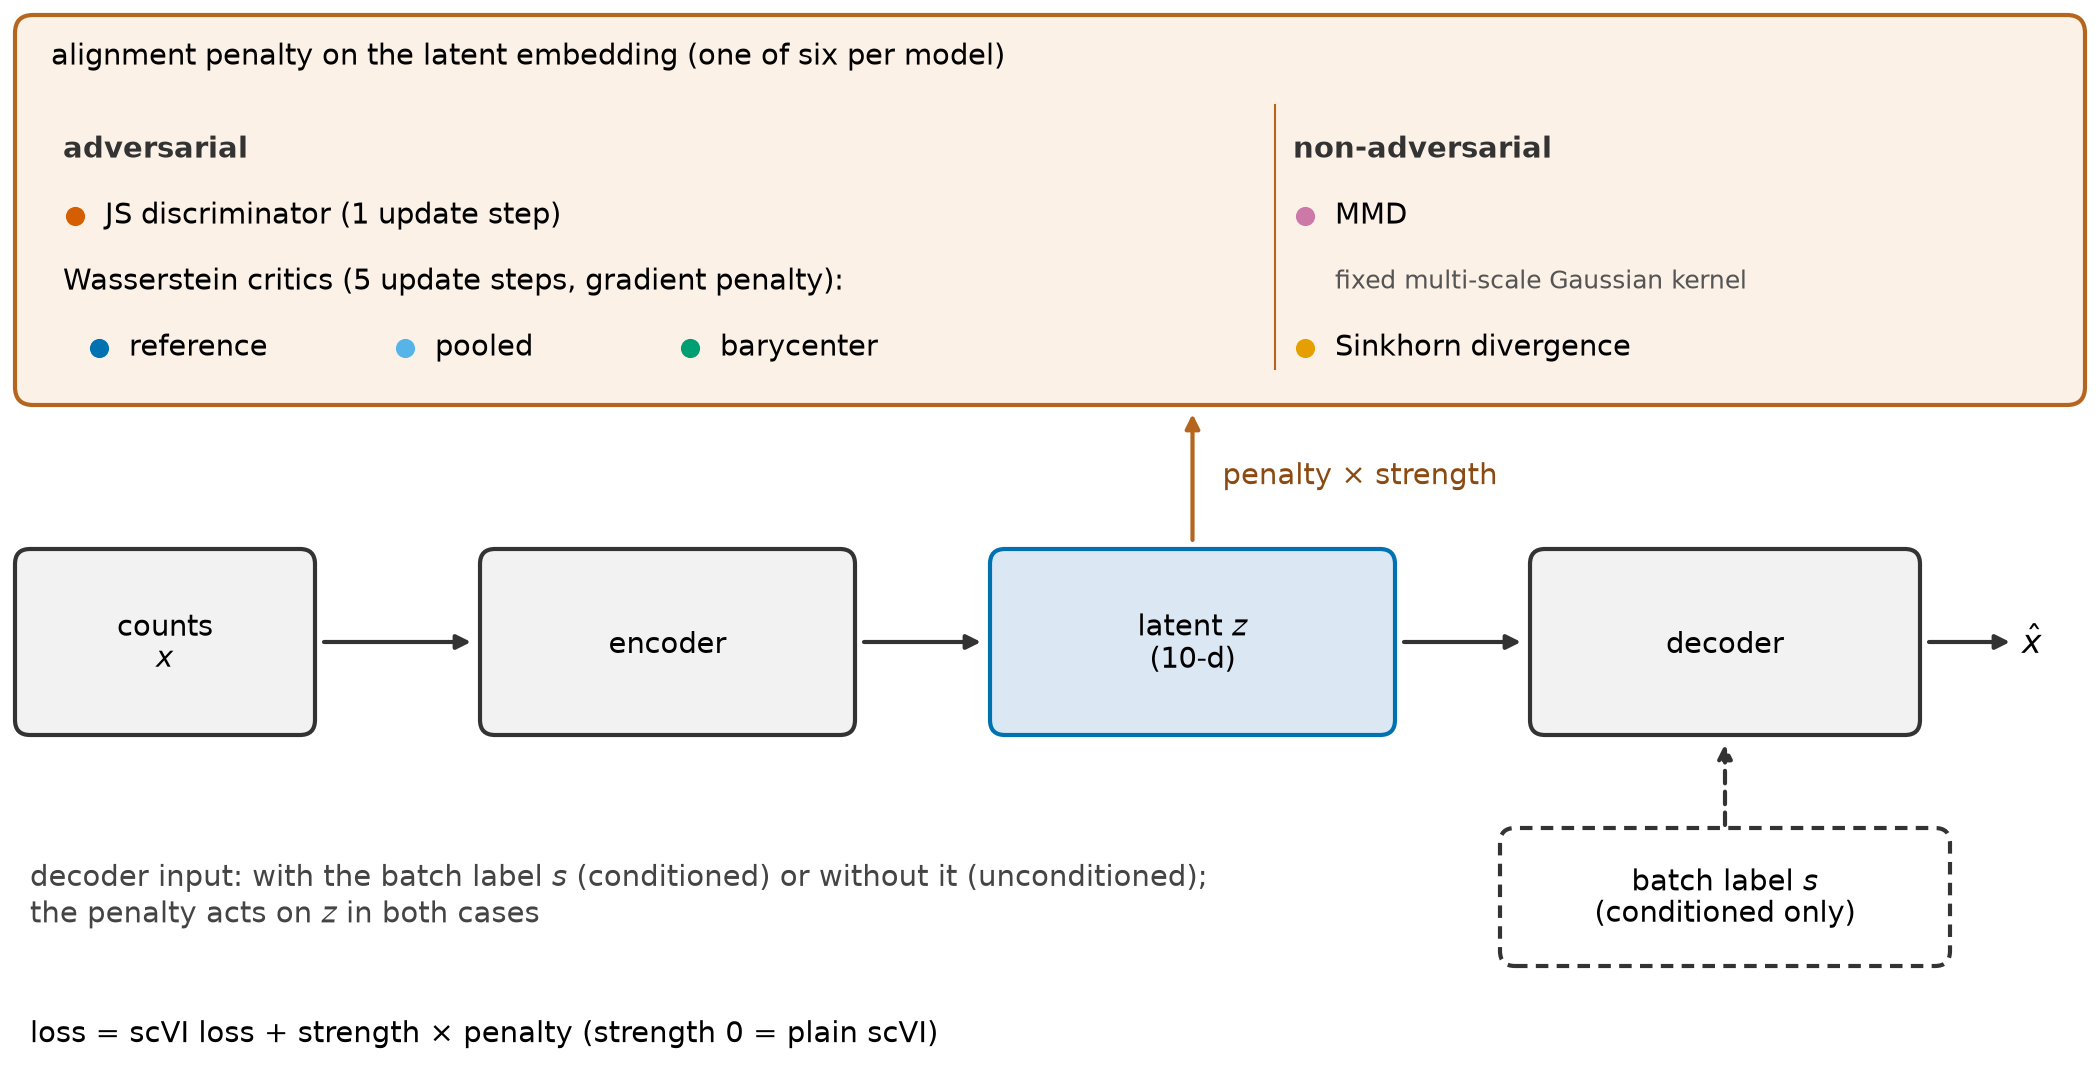
\includegraphics[width=\textwidth]{figures/fig1.png}
\caption{Model and read-out. (a) One scVI encoder--decoder is shared by all methods; the decoder receives the batch label (conditioned) or not (unconditioned), and only the alignment penalty on the 10-dimensional latent embedding is swapped. Four adversarial penalties (a Jensen--Shannon discriminator, one update step; Wasserstein critics, reference, pooled and barycenter, five update steps with a gradient penalty) and two non-adversarial penalties (MMD with a fixed multi-scale Gaussian kernel; the Sinkhorn divergence) are compared. The loss is the scVI loss plus the strength times the penalty; strength 0 is plain scVI. (b) One real task and decoder from the sweep, ATAC small with the unconditioned decoder, for three of the six penalties (colours as in Figures 2--6). Each curve joins plain scVI (star) and the sweep strengths in increasing order (10 strengths for the reference critic and MMD, 12 for the discriminator, which has two further low strengths); each point is a mean over the three seeds. Biology is read where the curve first reaches the matched batch removal $b^*$ (dashed line, 0.522), interpolating between neighbouring strengths (open circles; dotted arrows read the biology score): JS discriminator 0.666, reference critic 0.659, MMD 0.692. The discriminator and reference-critic curves cross $b^*$ a second time at higher strengths; the reading uses the first crossing.}
\label{fig:1}
\end{figure}


% This should be in supplement
% DONE: moved to Supplementary Note 2
% Two differences are by design: the discriminator takes one update step per training step with the generator's optimiser settings, whereas the critics take five steps with their own Adam settings (learning rate $10^{-4}$, betas 0 and 0.9).
% (10 latent dimensions, one hidden layer of 128 units, a zero-inflated negative binomial likelihood; Supplementary Table S2 and Supplementary Note 2),
% Plain scVI is the same model at strength zero. The adversary reads the encoder's posterior mean without per-dimension standardisation, two defaults kept after pilots whose switching rules were specified before scoring (Supplementary Note 2), and every fit is scored on the posterior mean.

% ---- Paragraph 2: penalties (user paragraph 2) ----

% This should be in supplement each trained with a gradient penalty of weight 10
% DONE: moved to Supplementary Note 1

\qquad Each method adds a fixed penalty, weighted by a fixed strength, to the scVI loss (Supplementary Table~\ref{tab:1}). The discriminator predicts each cell's batch and the encoder minimizes scvi-tools' bounded fool loss, a Jensen--Shannon (JS) type objective \citep{goodfellow2014generative}. We test three Wasserstein-1 (W1) critics \citep{arjovsky2017wasserstein,gulrajani2017improved}: reference, pooled and barycenter. The reference critic aims to align all batches with one reference batch, the batch with the highest cell-type entropy (the Shannon entropy of a batch's cell-type proportions, computed from the cell-type labels; ties go to the larger batch). The entropy rule prefers the batch whose cell types are most evenly represented, so that the target does not favour a few cell types, as a merely large batch, the other obvious choice, may do when a few cell types dominate it. The chosen reference holds every cell type in five of the eight tasks, and 10 of 17 (lung), 14 of 19 (human--mouse immune) and 3 of 4 (simulation 2) in the others, so in those three tasks some cells of other batches have no cell of their type in the reference. The pooled critic compares each batch with the cells of all other batches pooled together. The barycenter critic \citep{cuturi2014fast} estimates an average distribution of the batches present in each minibatch, recomputed at every step, and aligns every batch to it. The network-free penalties are the maximum mean discrepancy (MMD) of each batch to the others, with a fixed multi-scale Gaussian kernel \citep{gretton2012kernel}, and the debiased Sinkhorn divergence, an entropy-regularised optimal transport (OT) distance \citep{cuturi2013sinkhorn,genevay2018learning,feydy2019interpolating}, which at the smoothing used is not an estimate of W1. Loss equations and training settings are in Supplementary Notes 1 and 2.

% This level of detail should be in the supplement
% DONE: moved to Supplementary Note 3
% fit on its posterior-mean embedding, on all cells, with scIB's metrics unscaled, and summarise them as

% ---- Paragraph 3: data and metrics (user paragraph 3) ----
\qquad We benchmark the methods on eight integration tasks of the single-cell integration benchmark (scIB) \citep{luecken2022benchmarking}, used as distributed with their batch and cell-type labels: six real datasets from different biological settings, four of single-cell RNA sequencing (human pancreas, lung, immune cells, and joint human--mouse immune cells) and two of chromatin accessibility (assay for transposase-accessible chromatin, ATAC; mouse brain, a small and a large dataset, as gene-activity matrices), and two simulated datasets (Supplementary Table S1). RNA tasks use 2,000 highly variable genes and the ATAC tasks all features; counts are used as distributed.  We score each method with the scIB batch, biology and aggregate selection scores (formulas in Supplementary Note 3). The batch score is the mean of five metrics: principal-component regression on batch, batch average silhouette width (ASW), graph integration local inverse Simpson's index (iLISI), graph connectivity and the k-nearest-neighbor batch-effect test (kBET). The biology score is the mean of the task's biology metrics: normalized mutual information and adjusted Rand index between clusters and cell-type labels, cell-type ASW, isolated-label F1, isolated-label silhouette, graph cell-type LISI (cLISI), plus cell-cycle conservation on the four real RNA tasks and trajectory conservation on the two immune tasks, which have pseudotime. The  scIB combined selection score is the weighted average $0.4\,\mathrm{batch} + 0.6\,\mathrm{biology}$.

% ---- Paragraph 4: penalty-strength sweep (user paragraph 4; Pass 4 replaces the strength-pilot paragraph; the old argument shows the Pass 3 text with its earlier markup accepted) ----
\qquad \textbf{Penalty-strength sweep.} We fit plain scVI and the six penalties on all eight tasks at ten strengths in half-decade steps from 0.1 to 3,000 (0.1, 0.3, 1, 3, 10, 30, 100, 300, 1,000 and 3,000), with both decoders and three seeds (100--102). Two edge strengths were added in two places, 0.01 and 0.03 for the discriminator with the unconditioned decoder and 10,000 and 30,000 for the Sinkhorn divergence with the conditioned decoder, where a strength-choice rule (below) reached the end of the grid on the first three tasks fitted (the small chromatin-accessibility, immune and simulation 1 tasks). Each task therefore has 378 fits: 6 of plain scVI, 360 of the six penalties at ten strengths with three seeds and two decoders, and 12 at edge strengths; 3,024 fits in all. Nine further fits from an earlier strength-extension round, at strength 0.03 for the discriminator, the reference critic and the pooled critic on the immune task with the conditioned decoder, are also read, so the analysis uses 3,033 fits; that pair is low-signal and not ranked (Supplementary Note 4). A fit fails if its training loss or its latent becomes non-finite; failed fits are counted and left out of seed means (Supplementary Table S5). The sweep was planned as a pilot whose seed means would choose, by rules fixed before it ran, six strengths per penalty family and decoder for a planned fixed-strength benchmark at five new seeds; that benchmark was not run, so the rules select nothing and every analysis below reads all strengths of the sweep. The comparison is therefore exploratory: it describes  each penalty  over its whole strength range on these tasks and tests no hypothesis fixed in advance.

% ---- Paragraph 4b: replication across training seeds (Pass 5; sources in paper/pass5_changelog.md) ----
\qquad \textbf{Replication across training seeds.} A smaller replication across training seeds replaced the planned fixed-strength benchmark. It asks whether the sweep's readings at matched batch removal (the  matched level $b^*$ is defined in the next paragraph), which rest on three seeds per strength, hold on new fits. For every task and decoder pair that is ranked (13 of 16; the three low-signal pairs, immune, simulation 1 and simulation 2 with the batch-conditioned decoder, are skipped) and every penalty, we refitted with five new seeds (0--4) the two sweep strengths that bracket the first crossing of $b^*$ on the sweep's seed-mean curve, with $b^*$ fixed at its sweep value; 46 of these 78 curves cross $b^*$ more than once, and the first crossing sets the bracket, as in the sweep reading. In one cell the first crossing lies between plain scVI and the lowest sweep strength, so plain scVI at the new seeds is its lower point. Plain scVI was refitted at the same five seeds on every task and decoder. This gives 855 fits, 775 with a penalty and 80 of plain scVI (Supplementary Note 4). The strengths were chosen from the sweep's batch scores alone, never from its biology scores. Each task's replication fits are made on the same kind of machine as its sweep fits and scored with the same scoring code; for  lung, simulation 2 and pancreas the sweep fits were scored on the workstation and the replication fits on the cluster, under the sweep's rule for combining the two sites (Supplementary Note 11). The reading is the sweep's: on the means over the new seeds, biology at $b^*$ by linear interpolation in batch score between the two bracketing strengths, walking up from plain scVI at the new seeds and taking the first crossing. If the new means do not bracket $b^*$, the next sweep strength outward is fitted once with five seeds; if $b^*$ is still not bracketed, the penalty takes the bottom rank in that pair and is marked as not replicating the crossing. The sweep's readings and ranks were written down as the prediction, and the agreement rule was fixed, before any replication fit was scored (Supplementary Notes 4 and 10). The replication agrees with the sweep if two conditions hold: each of the four within-pair differences of 0.04 or more in the sweep keeps its sign on the new seeds, and the mean over the 13 ranked pairs of Kendall's rank correlation ($\tau_b$) between the sweep ranks and the replication ranks of the six penalties is above zero by a one-sided sign-flip permutation test over pairs (all $2^{13}$ sign patterns, $p<0.05$). The sign-flip test assumes that the 13 pairs' correlations are independent and symmetric about zero when the two orders are unrelated; this holds only roughly, because the two decoders of a task use the same task data and some tasks are related (two nested pairs), so its $p$-value is approximate. Two sensitivity analyses were added after the rule was fixed and are reported beside it, not as part of it. The first flips the signs per task, both decoders of a task together (all $2^{8}$ sign patterns over the eight tasks); because it still flips the two tasks of a nested pair separately, its $p$-value is approximate too. The second  flips the signs per task family, so that the two tasks of each nested pair and both decoders flip together (all $2^{6}$ sign patterns over six families: the two nested pairs, pancreas, lung, simulation 1 and simulation 2, which share no data); it handles the nesting but not other dependence between tasks, so it is approximate as well. Also beside the rule, and not part of it, we report the share of sweep near-ties (differences under 0.02) whose replication difference stays within $\pm0.04$, the rank correlation per pair, and the batch score that every replication point reached. Sweep (seeds 100--102) and replication (seeds 0--4) readings are reported separately. Because the rule tests only the sign of the within-pair differences of 0.04 or more and no precision calculation was made,  the replication is not set up to separate penalties whose readings differ by less; because it refits the same eight tasks, it says nothing about other data.

% This should be in the supplement
% DONE: moved to Supplementary Note 11 (run counts) and Table S5
% (480 fits each), 3,000 fits in all; a fit fails if its training loss or its latent becomes non-finite}{5 seeds}.

% ---- Paragraph 5: matched batch removal (user paragraph 5; Pass 4 deletes the main-benchmark sentences) ----
\qquad Strength has a different scale for each penalty, and a stronger penalty trades biology for batch removal along a curve, as Li et al.\ showed for scVI \citep{li2022trade}, so we do not compare methods at a fixed strength. Instead, for each task and decoder we set a batch score, $b^*$, halfway between plain scVI's mean batch score and the highest mean batch score that every one of the six penalties reaches at a sweep strength with no failed fit (Supplementary Note 5), and read each penalty's biology score at $b^*$, a batch removal that every penalty reaches (Figure 1b). This matched level works only  if the penalties remove clearly more batch effect than plain scVI. A task and decoder pair is low-signal when that gap is under 0.02, so that $b^*$ sits less than 0.01 above plain scVI and cannot be placed reliably; low-signal pairs are left out of the ranking and shown in a separate table. In the sweep the low-signal pairs are  the immune task and both simulations with the batch-conditioned decoder (gaps in Results); no pair is low-signal with the unconditioned decoder.

% % ---- New paragraph (a): statistical analysis (from Meth-7, Meth-9, Meth-11; PREREG, SPEC) ----
% This section is too focused on the critic vs discriminator, it needs to be generalized to the new benchmark.
% \added{\qquad The primary comparison is the reference critic's biology score at $b^*$ minus the discriminator's, per task and decoder, read by linear interpolation on each method's curve of seed-mean scores from plain scVI through its six strengths, with uncertainty from repeating the reading with each seed left out (Supplementary Note 5 gives the rules for when a task is evaluable). The six real tasks are pooled in one model that weights each task by its uncertainty and lets related tasks share a family effect, because the human--mouse immune task contains all immune cells and the large chromatin-accessibility task contains all cells of the small one; the priors have scale 0.1, the model is integrated exactly, and simulations are reported per task and never pooled. We declare a direction if the posterior probability that the overall difference lies beyond a margin of 0.01 on one side is at least 0.95, practical equivalence if the probability that it lies within $\pm0.01$ is at least 0.95, and otherwise the result is inconclusive \citep{corani2017statistical}. The six primary results (this comparison, the trade-off area and the collapse rate, each per decoder) are judged on their own posteriors; an exact Wilcoxon signed-rank test with Holm's correction over the six is reported as description only, because with six tasks its smallest attainable $p$, 0.031, exceeds the first threshold of $0.05/6$. From the pilot, the minimal detectable effect at 80\% power is 0.131 over the six real tasks, so the design is underpowered. The pilot rules were frozen on 4 October 2026, their amendments and this analysis on 16 October 2026, before anyone had read a main-benchmark score, and the analysis runs once (Supplementary Note 11).}

\qquad The main analysis is a descriptive ranking. For each task and decoder, a penalty's curve joins plain scVI and its sweep strengths (ten, or twelve where edge strengths were fitted) by seed-mean scores over the three seeds (100--102), and its biology score is read at $b^*$ by linear interpolation where the curve first reaches $b^*$ (Figure 1b). The uncertainty of each reading is its standard error  over repeats with each of the three seeds left out in turn, holding $b^*$ fixed and leaving the same seed out of plain scVI, together with the range (lowest to highest) of the penalty's rank over the three repeats. Both are reported only if at least two of the three leave-one-seed-out readings exist, and otherwise as not available; the penalty is ranked either way (Supplementary Note 6).  Within each ranked (not low-signal) pair the six penalties are ordered by biology at $b^*$ (rank 1 is best), tied penalties getting the average of their ranks. A penalty whose curve does not reach $b^*$ takes the bottom rank in that pair, penalties that all fail sharing the last places, following scIB, where methods that could not be run on a task were given the same rank as unintegrated data \citep{luecken2022benchmarking}. As in scIB, the mean rank over all real tasks that are not low-signal is reported for each decoder; simulations are ranked and reported  separately  (Supplementary Note 6). We report no significance tests: ranks and their uncertainty describe the data. Each penalty's selection score is also compared with plain scVI's, at one strength not tuned on the task and as the expected best of $k$ tries (below). The ranking rules were written for the planned fixed-strength benchmark and are applied to the sweep with the changes listed in Supplementary Note 10. The three tasks fitted first had already been read by the strength-choice rules, whereas no sweep score of the other five tasks existed when the ranking rules were written (dated 22 and 23 October 2026; both commits were made on 22 October), although score files of some baseline fits on four of them are older, from 6 to 12 October (Supplementary Notes 10 and 11).

% ---- New paragraph (b): baselines (from Meth-2, Meth-13; paper.tex 436-447; SPEC section 9) ----
\qquad We place the penalties against plain scVI and against standard tools: scvi-tools' own adversarial classifier (its built-in batch classifier, run with the conditioned decoder only), Harmony \citep{korsunsky2019fast}, Scanorama \citep{hie2019efficient}, sysVI \citep{hrovatin2025integrating}, scANVI, which uses the cell-type labels \citep{xu2021probabilistic}, and principal-component analysis (PCA) as the uncorrected reference. The comparison allows for the outcome that no alignment penalty improves on plain scVI. Harmony, Scanorama and sysVI run at six settings each, scANVI and PCA at one (settings, seeds and fit counts in Supplementary Table S4 and Supplementary Note 8).  The scvi-tools adversary, scANVI and sysVI are fitted with five seeds (0--4), and Harmony, Scanorama and PCA once per setting, all on every task: 448 planned fits (447 fitted and scored; Results), including three sensitivity settings (Harmony at 50 principal components, Scanorama at 100 dimensions and PCA at 50 components). Because the penalties and the tools have different numbers of settings, placement compares methods at equal numbers of tries (a try is one setting of a method, fitted and scored), by the expected best selection score among $k$ settings drawn at random, and is descriptive. Each penalty is also scored at one strength not tuned on that task, the strength with the best mean selection score on the real tasks of the other task families, shown beside the task's own best strength as an optimistic bound (Supplementary Note 7); Harmony, Scanorama and sysVI get their setting by the same rule, with the task's own best setting  as the optimistic bound (Supplementary Note 8). scANVI and PCA run at one setting, so they involve no choice.

% ---- New paragraph (c): follow-up experiment (from Meth-14 to Meth-16; PREREG 721-790; SPEC-FU) ----

% This section is too focused on critic vs distriminator.
% DONE: dropped (first author's decision)
% \added{\qquad A follow-up experiment asks whether any critic--discriminator gap comes from the divergence itself or from the regularisation, optimiser and update steps that also differ between the two. On the small chromatin-accessibility, immune and pancreas tasks, with both decoders and three fresh seeds (10--12), it fits nine settings: the discriminator plain, with spectral normalisation \citep{miyato2018spectral}, with an R1 gradient penalty, a penalty on the discriminator's gradient at real data only \citep{mescheder2018training}, and with spectral normalisation plus the critics' Adam settings, each at one step; and the pooled critic with gradient penalty at 1, 5 and 10 steps and with spectral normalisation at 1 and 5 steps (Table 1, Supplementary Table S5). Each setting runs at three strengths, its base method's matched strength on the main benchmark (the strength whose batch score is nearest $b^*$) and the two grid neighbours, so the follow-up starts only after the main benchmark is scored: 486 fits. One contrast per decoder is confirmatory, the spectrally normalised pooled critic minus the spectrally normalised discriminator with the critics' optimiser, both at one step, which differ only in the loss and its target. Biology is read at $b^*$ where a setting's three strengths bracket it, pooled with the same model, margin and 0.95 rule, with Holm's correction over the two results; the divergence is said to explain the main gap only if the primary comparison and this contrast have a declared direction of the same sign and every regularisation and step-count contrast is smaller (Supplementary Note 9). Because both arms of this contrast inherit strengths chosen for other settings, a pre-check of 36 fits (18 per arm, on the pilot tasks at seed 100) decides by a rule fixed in advance whether each arm's three strengths move one half-decade step up, move down or stay: \tbd{pre-check outcome for each arm}.}

\qquad For each penalty we also report four descriptive views: collapse rate,  hypervolume, share of non-dominated strengths,  and label transfer (rules in Supplementary Notes 7 and 9). A fit collapses if it fails or its biology score is at least 0.10 below the same seed's plain scVI; the collapse rate is the collapsed share of a penalty's fits in a task and decoder at strengths whose mean batch score is at most the highest common batch score (the range of Figure 4; all strengths in Supplementary Table S8), with exact binomial (Clopper--Pearson) 95\% intervals \citep{clopper1934use}, which are nominal because the fits of one seed are judged against one plain-scVI threshold and are not independent (Discussion).  The hypervolume \citep{zitzler1998multiobjective}, which Li et al.\ used to compare trade-off fronts \citep{li2022trade}, is the area of the batch-score by biology-score plane that a penalty's sweep points reach beyond a reference point at plain scVI's batch score and 0.10 below its biology score, with batch scores above the highest common batch score counted at it so that every penalty is measured over the same batch range, divided by the batch gap that sets $b^*$ so that tasks share one scale; it is the area under the penalty's Pareto frontier, the best biology among its strengths at or beyond each batch level (Figure 4; uncapped values in Supplementary Table S8). The share of non-dominated strengths, also from Li et al., is the fraction of a penalty's strengths that none of its other strengths beats on both the batch and the biology score.

\qquad  Label transfer holds each batch out in turn and predicts its cell types from the other batches with a 15-nearest-neighbour classifier, on each penalty's embedding at the strength whose batch score is nearest $b^*$, never chosen by accuracy (Supplementary Note 9).

\qquad A direct biology check reads four per-cell-type quantities on the saved embeddings, with no new fits: neighbourhood purity, the share of a cell's 15 nearest neighbours in the latent space that carry its own cell-type label, averaged within each type; the same purity and the label-transfer recall for rare types, those with under 1\% of a task's cells; marker-gene preservation, the Jaccard overlap between each type's top 20 markers from the expression as distributed and from the expression averaged over the 15 neighbours, on the four RNA tasks; and the label-transfer confusion table. Penalties are read at the label-transfer strength and every baseline at each of its settings, and each value is reported as a difference from plain scVI. The check is exploratory: its rules were written after the sweep scores had been read and before any of its values was computed (Supplementary Note 12).

\qquad \emph{Use of large language models.} Large language model tools were used in this work: Claude (Anthropic), through the Claude Science and Claude Code applications, and Codex (OpenAI). They wrote and checked analysis, scoring and figure code; prepared, ran and monitored computational jobs on the workstation and the cluster; assisted with literature searches; checked the numbers in the text against their source files; reviewed the text independently; and drafted and edited text. The study design and the decisions about what was run, measured and reported were made or approved by the authors. All figures are drawn from the data by plotting scripts in the repository (no image was made by a generative model), and every number in the paper is re-read from its source file by a script (\texttt{paper/tools/check\_ledger.py}). The authors checked all outputs and take responsibility for the content.

\hd{Results}{1,500 words; 8 paragraphs plus one for the replication across training seeds and one for the direct biology check}
\pp{Res-1}{Which fits completed, and where batch removal could be matched.}
All 3,033 sweep fits and 447 of 448 baseline fits were scored, and every penalty reached $b^*$ in every task and decoder pair; the immune task and both simulations were low-signal with the batch-conditioned decoder (Supplementary Notes 5, 8 and 11; Supplementary Table S5).
\pp{Res-2}{Penalties are ranked by the biology they keep at matched batch removal (Figure 2; Supplementary Table \ref{tab:3}).}
The order of the penalties depended on the decoder: MMD had the fifth-best mean rank with the batch-conditioned decoder and the best with the unconditioned decoder, and the Sinkhorn divergence the second-best and the worst. With the batch-conditioned decoder, the ranking rested on five real tasks. Mean ranks (range across those tasks) were the pooled critic 2.20 (1--3); the Sinkhorn divergence 2.40 (1--5); the barycenter critic 3.00 (1--5); the reference critic 3.80 (1--5); MMD 4.60 (2--6); the discriminator 5.00 (3--6). With the unconditioned decoder, all six real tasks contributed: MMD 2.17 (1--6); the reference critic 3.33 (1--6); the pooled critic 3.33 (2--5); the discriminator 3.50 (1--5); the barycenter critic 4.00 (1--6); the Sinkhorn divergence 4.67 (3--6). The Sinkhorn divergence ranked first most often with the batch-conditioned decoder, on the human--mouse immune and lung tasks; the discriminator ranked last on the small chromatin-accessibility, lung and pancreas tasks. With the unconditioned decoder, MMD ranked first most often, on the large chromatin-accessibility, human--mouse immune and pancreas tasks; the reference critic ranked last on the small chromatin-accessibility and human--mouse immune tasks, and the Sinkhorn divergence on the large chromatin-accessibility and lung tasks.

% ---------------------------------------------------------------- Figure 2
\begin{figure}[!htbp]
\centering
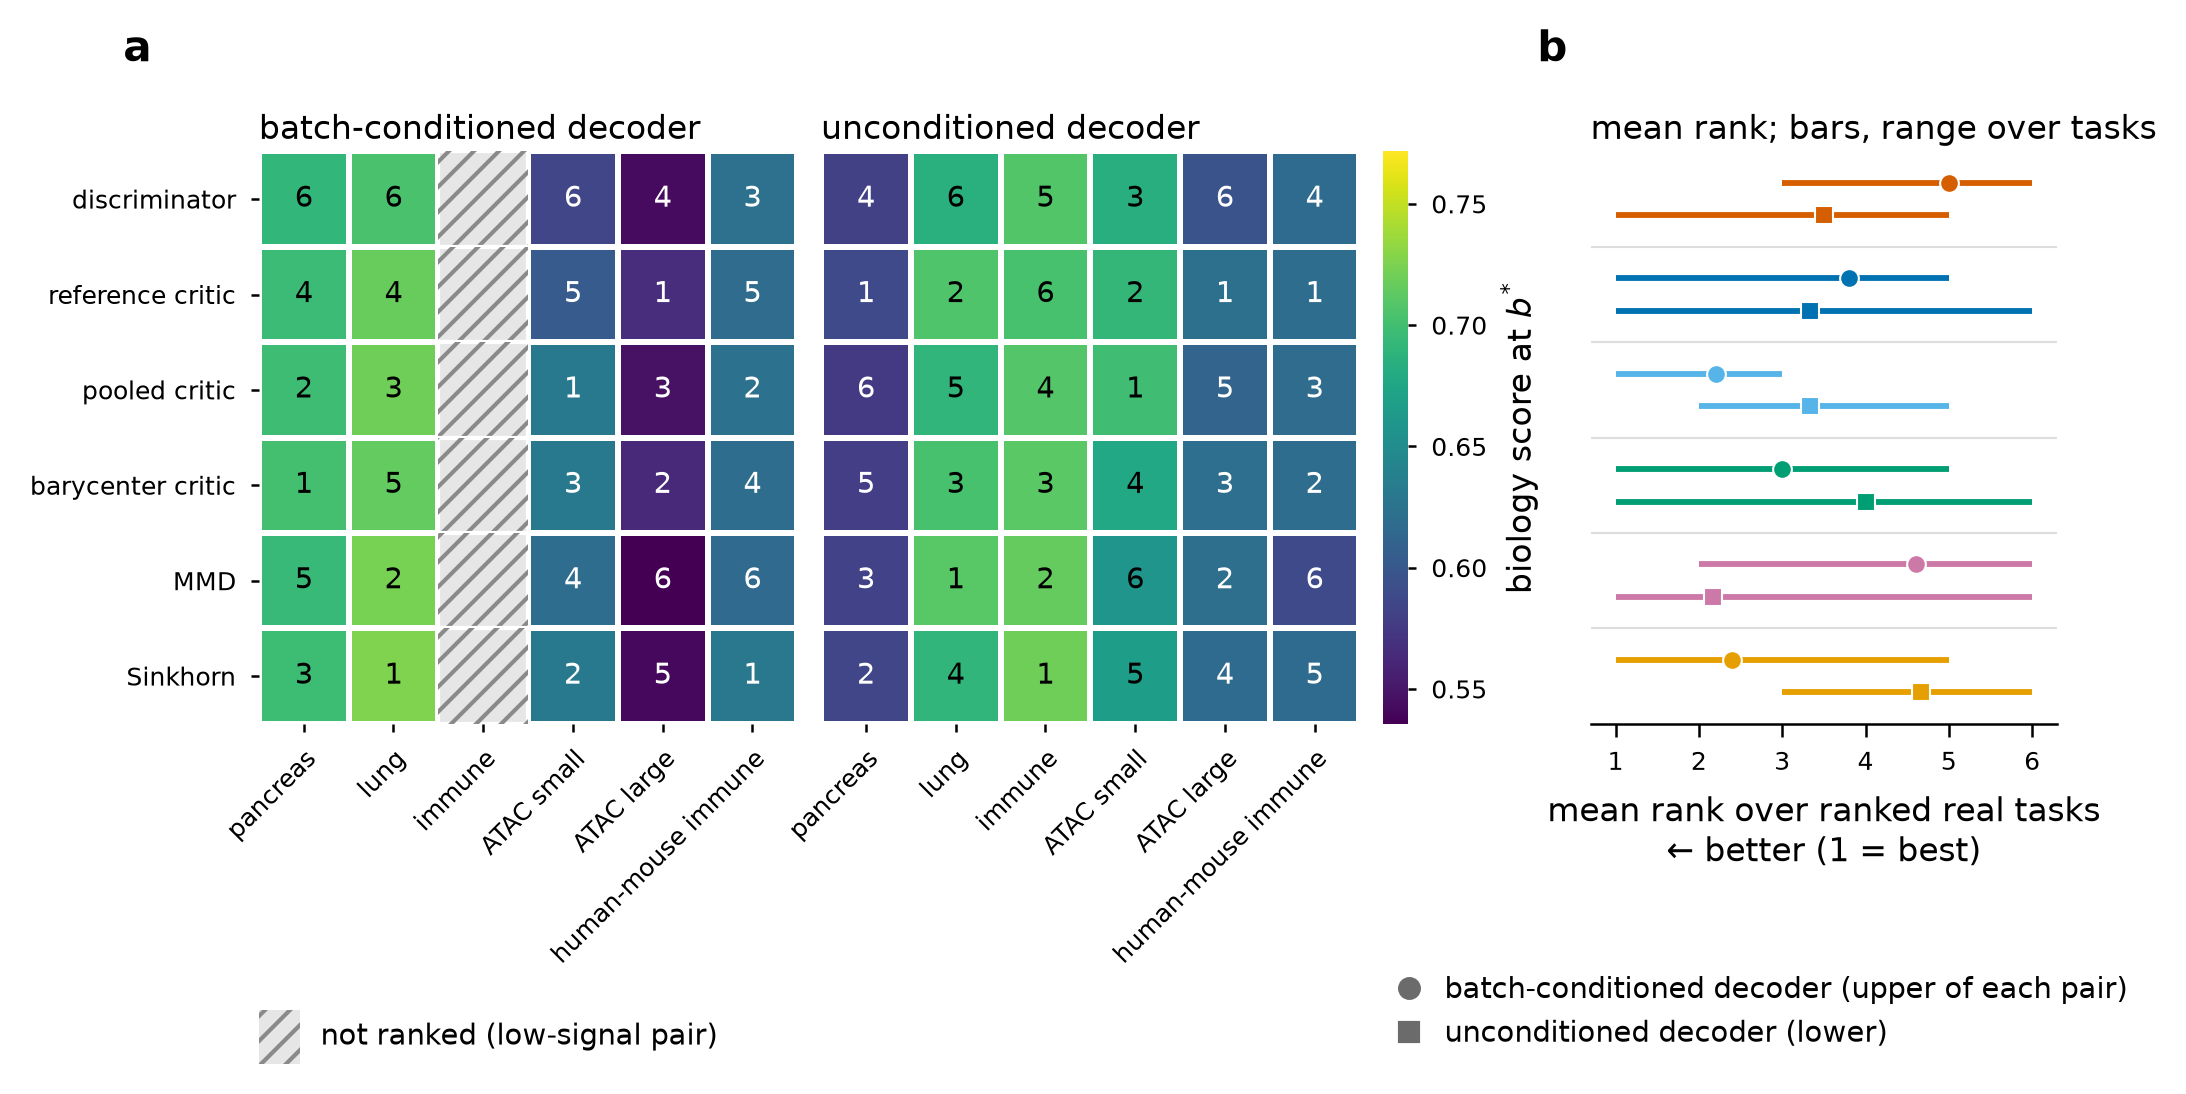
\includegraphics[width=\textwidth]{figures/fig2.png}
\caption{Ranking of the six penalties by biology kept at matched batch removal $b^*$. (a) Biology score at $b^*$ (colour) and rank among the six penalties within each task row (number; tied penalties share the average rank) for each real task, with the batch-conditioned decoder (upper block) and the unconditioned decoder (lower block). Hatched row: the immune task with the batch-conditioned decoder, a low-signal pair that is not ranked. A penalty whose curve does not reach $b^*$ would take the bottom rank; every curve reached it here. (b) Mean rank over the ranked real tasks (five with the batch-conditioned decoder, upper block; six with the unconditioned decoder, lower block), with the penalties of each decoder sorted from best to worst mean rank (the value after each name, rounded to one decimal); dot, mean rank; bar, lowest to highest rank over those tasks; the rank axis runs from 6 at the left to 1 (best) at the right. The pooled critic had the best mean rank with the batch-conditioned decoder (2.20) and MMD with the unconditioned decoder (2.17). The leave-one-seed-out standard error of each reading in (a) and the range of each rank over the three leave-one-seed-out repeats are in Supplementary Table S6. Simulations are ranked separately (Supplementary Figure S1).}
\label{fig:2}
\end{figure}


Most neighbouring readings were close. In 44 of the 55 pairs of penalties next to each other in a task's order (17 of 25 with the batch-conditioned decoder, 27 of 30 with the unconditioned decoder), the two biology readings differed by less than the larger of their leave-one-seed-out standard errors, and 2 of the 11 first places stayed first in all three leave-one-seed-out repeats (Methods; Supplementary Table S6). The simulations are ranked with the unconditioned decoder only, because both pairs with the batch-conditioned decoder were low-signal (Supplementary Figure S1).
\pp{Res-2b}{The replication across training seeds reports whether the sweep's readings at $b^*$ hold on new fits (Supplementary Table S9).}
A replication on 895 new fits (seeds 0--4) met its agreement rule only after the extension step that the rule prescribes: all four large sweep gaps kept their sign, and the sweep and replication orders were positively correlated (mean Kendall's $\tau_b$ 0.456, $p=0.00049$). The first-ranked penalty changed in 7 of 13 pairs, and by mean rank on the new seeds the Sinkhorn divergence led with the batch-conditioned decoder (2.20) and the pooled critic with the unconditioned decoder (2.67) (Supplementary Note 13, Supplementary Table S9).
\pp{Res-3}{Figure 3 compares the biology each penalty keeps at the matched level with the biology it keeps at its strongest setting.}
The penalties kept similar biology up to the matched level and differed at stronger settings (Figure 3; trade-off curves in Supplementary Figure S7, built as in Supplementary Note 5): over the 11 ranked real task and decoder pairs, biology at $b^*$ differed between penalties by a median of 0.025, against 0.213 at each penalty's strongest fitted setting. The barycenter critic reached the lowest biology score of the six penalties in all 12 real task and decoder pairs (0.287 to 0.516); on lung with the batch-conditioned decoder its strongest setting ended below plain scVI on both scores (batch 0.466 and biology 0.397, against 0.633 and 0.722). It also had the shortest batch-removal range on the large chromatin-accessibility task with the batch-conditioned decoder (highest batch score 0.674; the other penalties 0.683 to 0.834). With the unconditioned decoder, the chromatin-accessibility curves lost biology as batch removal increased, whereas on pancreas every penalty raised both scores over part of its strength range.

% ---------------------------------------------------------------- Figure 3
\begin{figure}[!htbp]
\centering
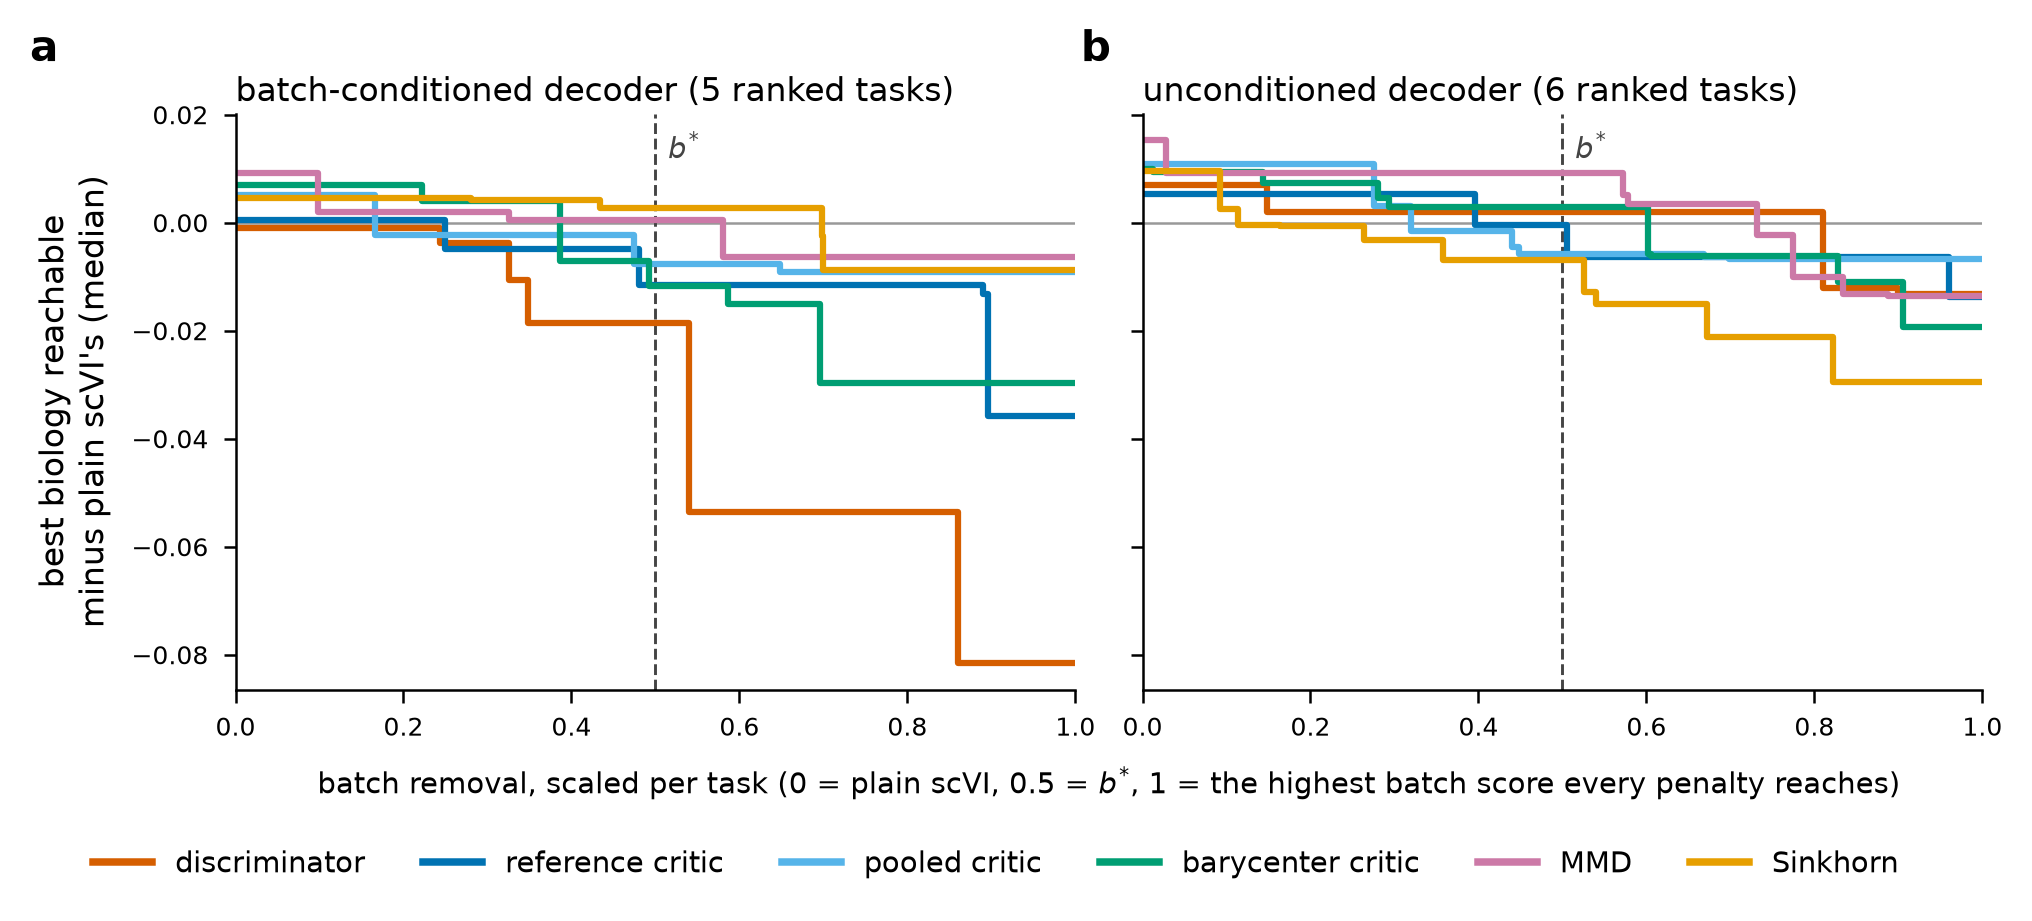
\includegraphics[width=\textwidth]{figures/fig3.png}
\caption{Biology kept by each penalty relative to plain scVI, at the matched batch removal $b^*$ (filled dots) and at the penalty's strongest fitted setting (open dots), with the batch-conditioned  (a) and the unconditioned decoder (b). One dot per real task: biology score minus plain scVI's with the same decoder (higher is better); grey line, no change. Filled dots are drawn for the ranked tasks only (the immune task with the batch-conditioned decoder is low-signal); open dots for all six real tasks. The full trade-off curves are in Supplementary Figure S7.}
\label{fig:3}
\end{figure}

\pp{Res-3b}{Each penalty's Pareto frontier gives the most biology it kept at each level of batch removal (Figure 4).}
We scaled batch removal per task and decoder so that 0 is plain scVI, 0.5 is $b^*$ and 1 is the highest batch score every penalty reaches, and took at each level the best biology among a penalty's strengths at that level or beyond (Methods). Up to $b^*$, the median frontier over the ranked real tasks stayed within 0.019 of plain scVI's biology for every penalty and decoder (Figure 4a,b). At the highest common batch score, the discriminator's median frontier with the batch-conditioned decoder was 0.082 below plain scVI, against 0.006--0.036 for the other penalties; with the unconditioned decoder, the six frontiers ended 0.007--0.029 below. The hypervolume up to that level, the area under a task's frontier above 0.10 below plain scVI's biology (0.10 when plain scVI's biology is kept throughout), had medians of 0.086--0.102 for every penalty and decoder except the discriminator with the batch-conditioned decoder, 0.063 (Figure 4c,d; Supplementary Table S8). The barycenter critic's batch removal ended at the highest common batch score in all 11 ranked pairs, so it set that level, whereas every other penalty reached beyond it in all 11 (Supplementary Note 7). Each frontier takes the best strength at each level after scoring, so it is optimistic, and differences of the size seen at $b^*$ were often within the leave-one-seed-out standard error (Res-2).

% ---------------------------------------------------------------- Figure 4 (Pass 23: Pareto frontier)
\begin{figure}[!htbp]
\centering
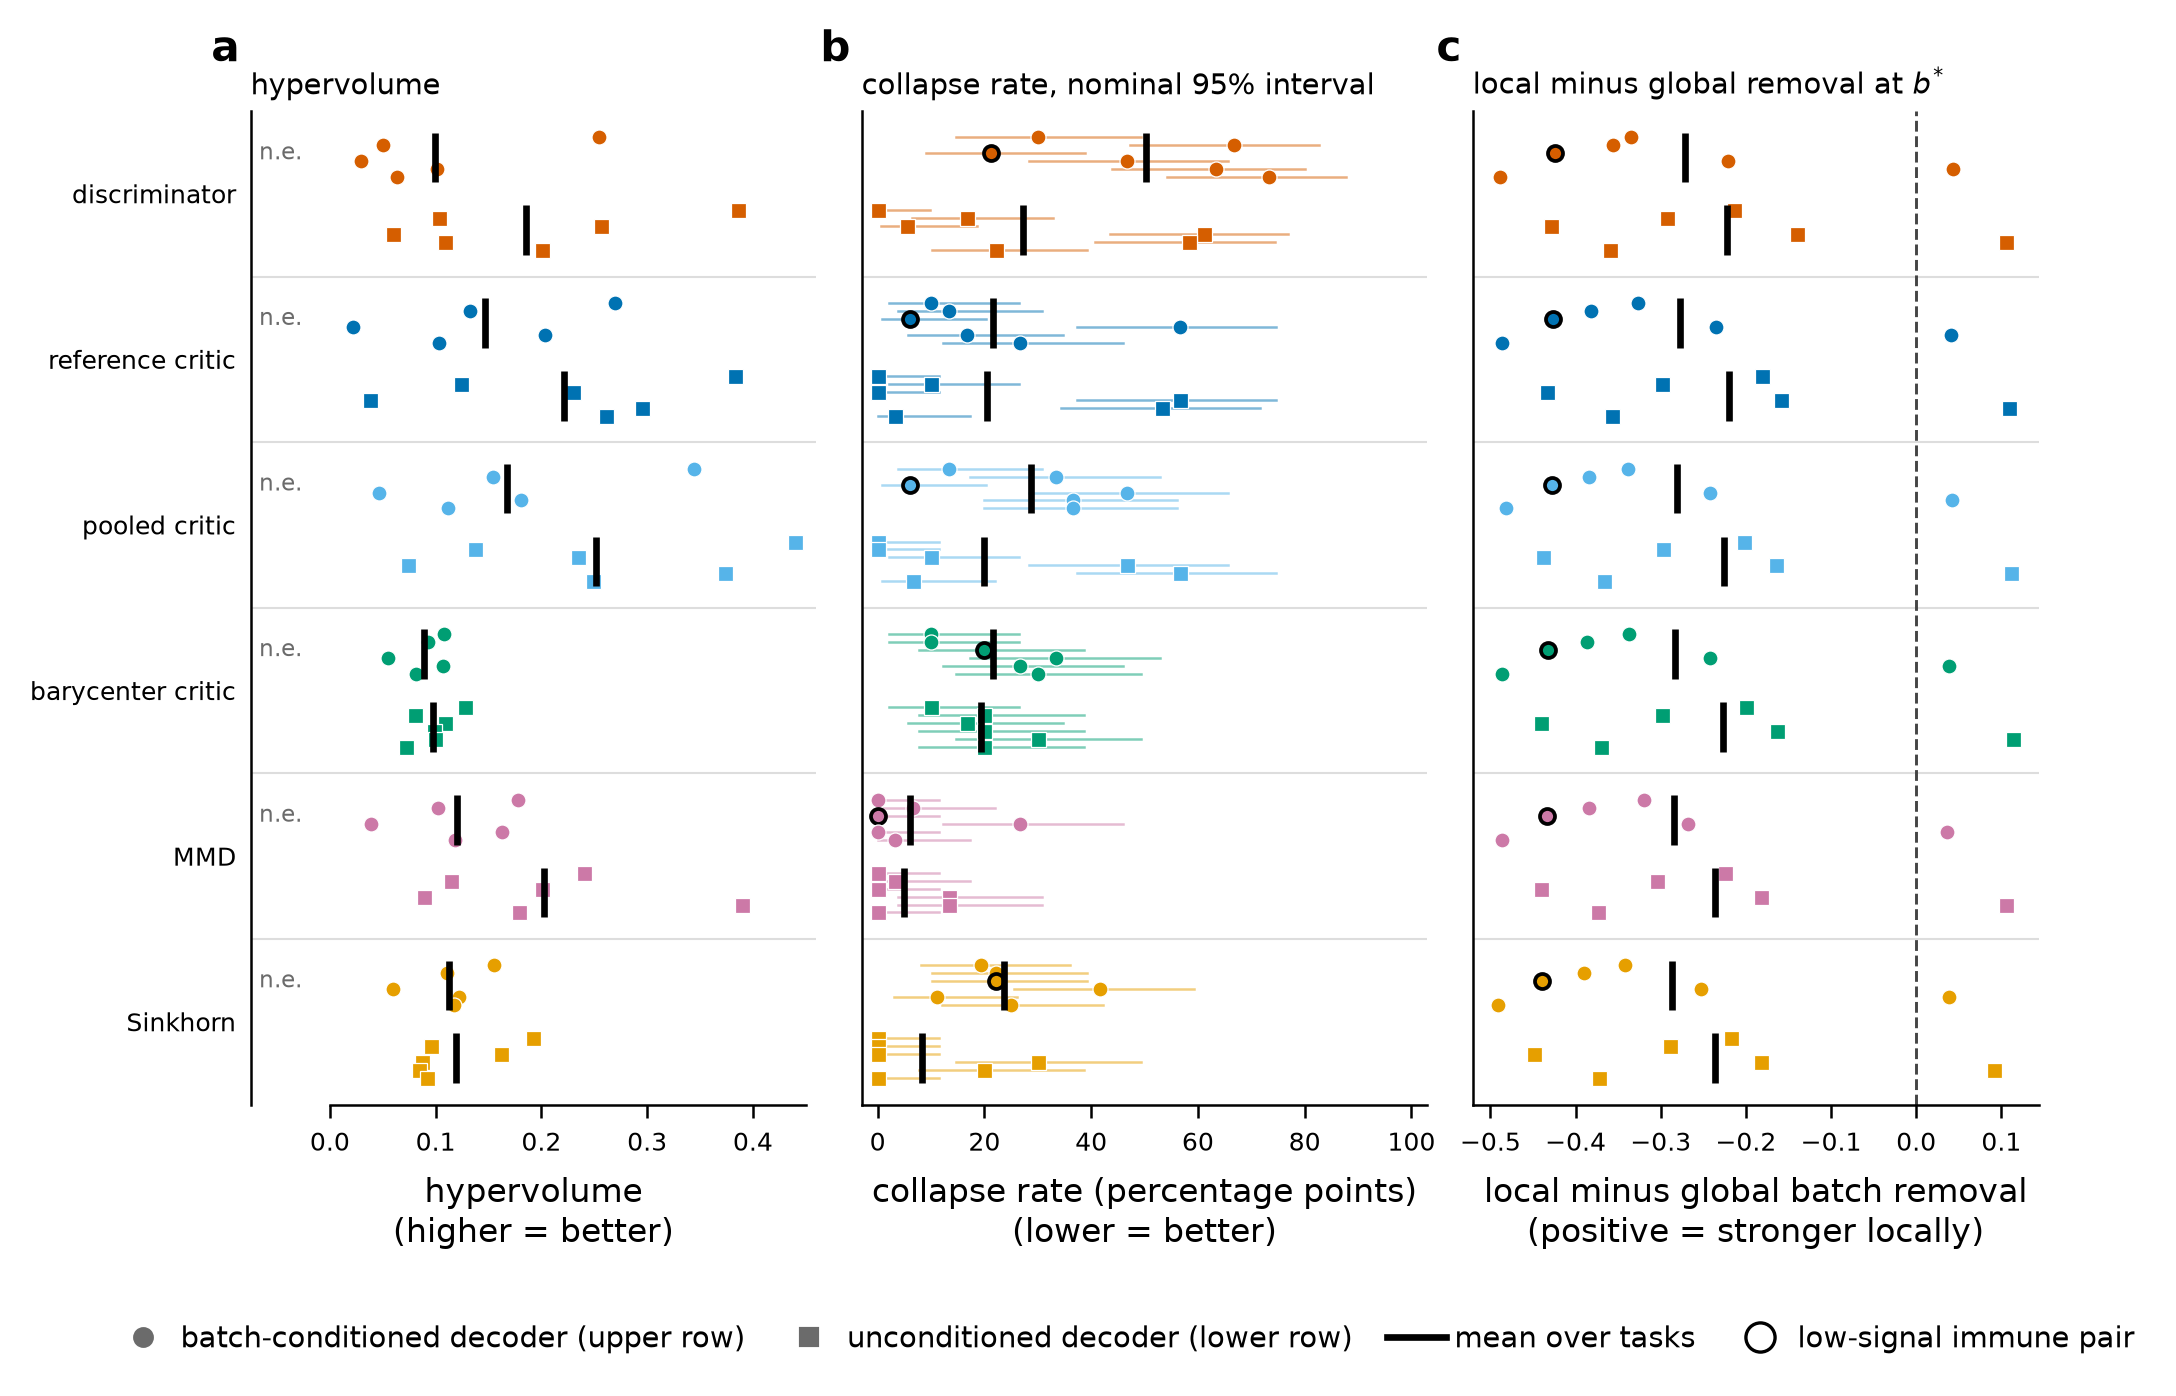
\includegraphics[width=\textwidth]{figures/fig4.png}
\caption{Pareto frontier of each penalty over the ranked real tasks (5 with the batch-conditioned decoder, a and c; 6 with the unconditioned decoder, b and d; the low-signal immune pair is excluded). Batch removal is scaled per task so that 0 is plain scVI, 0.5 is matched batch removal $b^*$ (dashed line) and 1 is the highest batch score every penalty reaches. (a, b) Best biology score reachable at each level or beyond, minus plain scVI's, median over tasks, from seed means over three seeds. (c, d) Hypervolume up to the highest common batch score, the area under each task's frontier above 0.10 below plain scVI's biology (higher is better; dashed line, 0.10, plain scVI's biology kept throughout); dots, tasks; black tick, median. The frontiers are assembled after scoring and are optimistic.}
\label{fig:4}
\end{figure}

\pp{Res-4}{The collapse rate counts how often a penalty's fits lose 0.10 or more biology (Figure 5; the share of non-dominated strengths is in Supplementary Table S8).}
We count the fits at strengths whose mean batch score is at most the highest common batch score, the range of Figure 4; rates over all strengths are in Supplementary Table S8 (Methods). With the batch-conditioned decoder, the median collapse rate over the six real tasks was 34\% for the discriminator, 24\% for the Sinkhorn divergence, 23\% for the barycenter critic, 21\% for the pooled critic, 11\% for the reference critic and 3\% for MMD; with the unconditioned decoder it was 20\% for the barycenter critic, 11\% for the discriminator, 10\% for the reference critic and 0\% for the other three. The highest rate with the batch-conditioned decoder was the discriminator's, 56\% (31\%--78\%, nominal 95\% interval) on the human--mouse immune task; the other five penalties peaked on the small chromatin-accessibility task. MMD collapsed less often than the discriminator on 5 of the 6 real tasks with that decoder, although it ranked above the discriminator at $b^*$ on only 3 of the 5 ranked tasks. Every collapse was a loss of biology; no fit failed. Over all strengths, 67 of the discriminator's 91 collapses with the batch-conditioned decoder and 47 of 59 with the unconditioned decoder lay beyond the highest common batch score, against none of the barycenter critic's, whose strongest setting sets that score. These summaries include the low-signal immune pair.

% ---------------------------------------------------------------- Figure 5
\begin{figure}[!htbp]
\centering
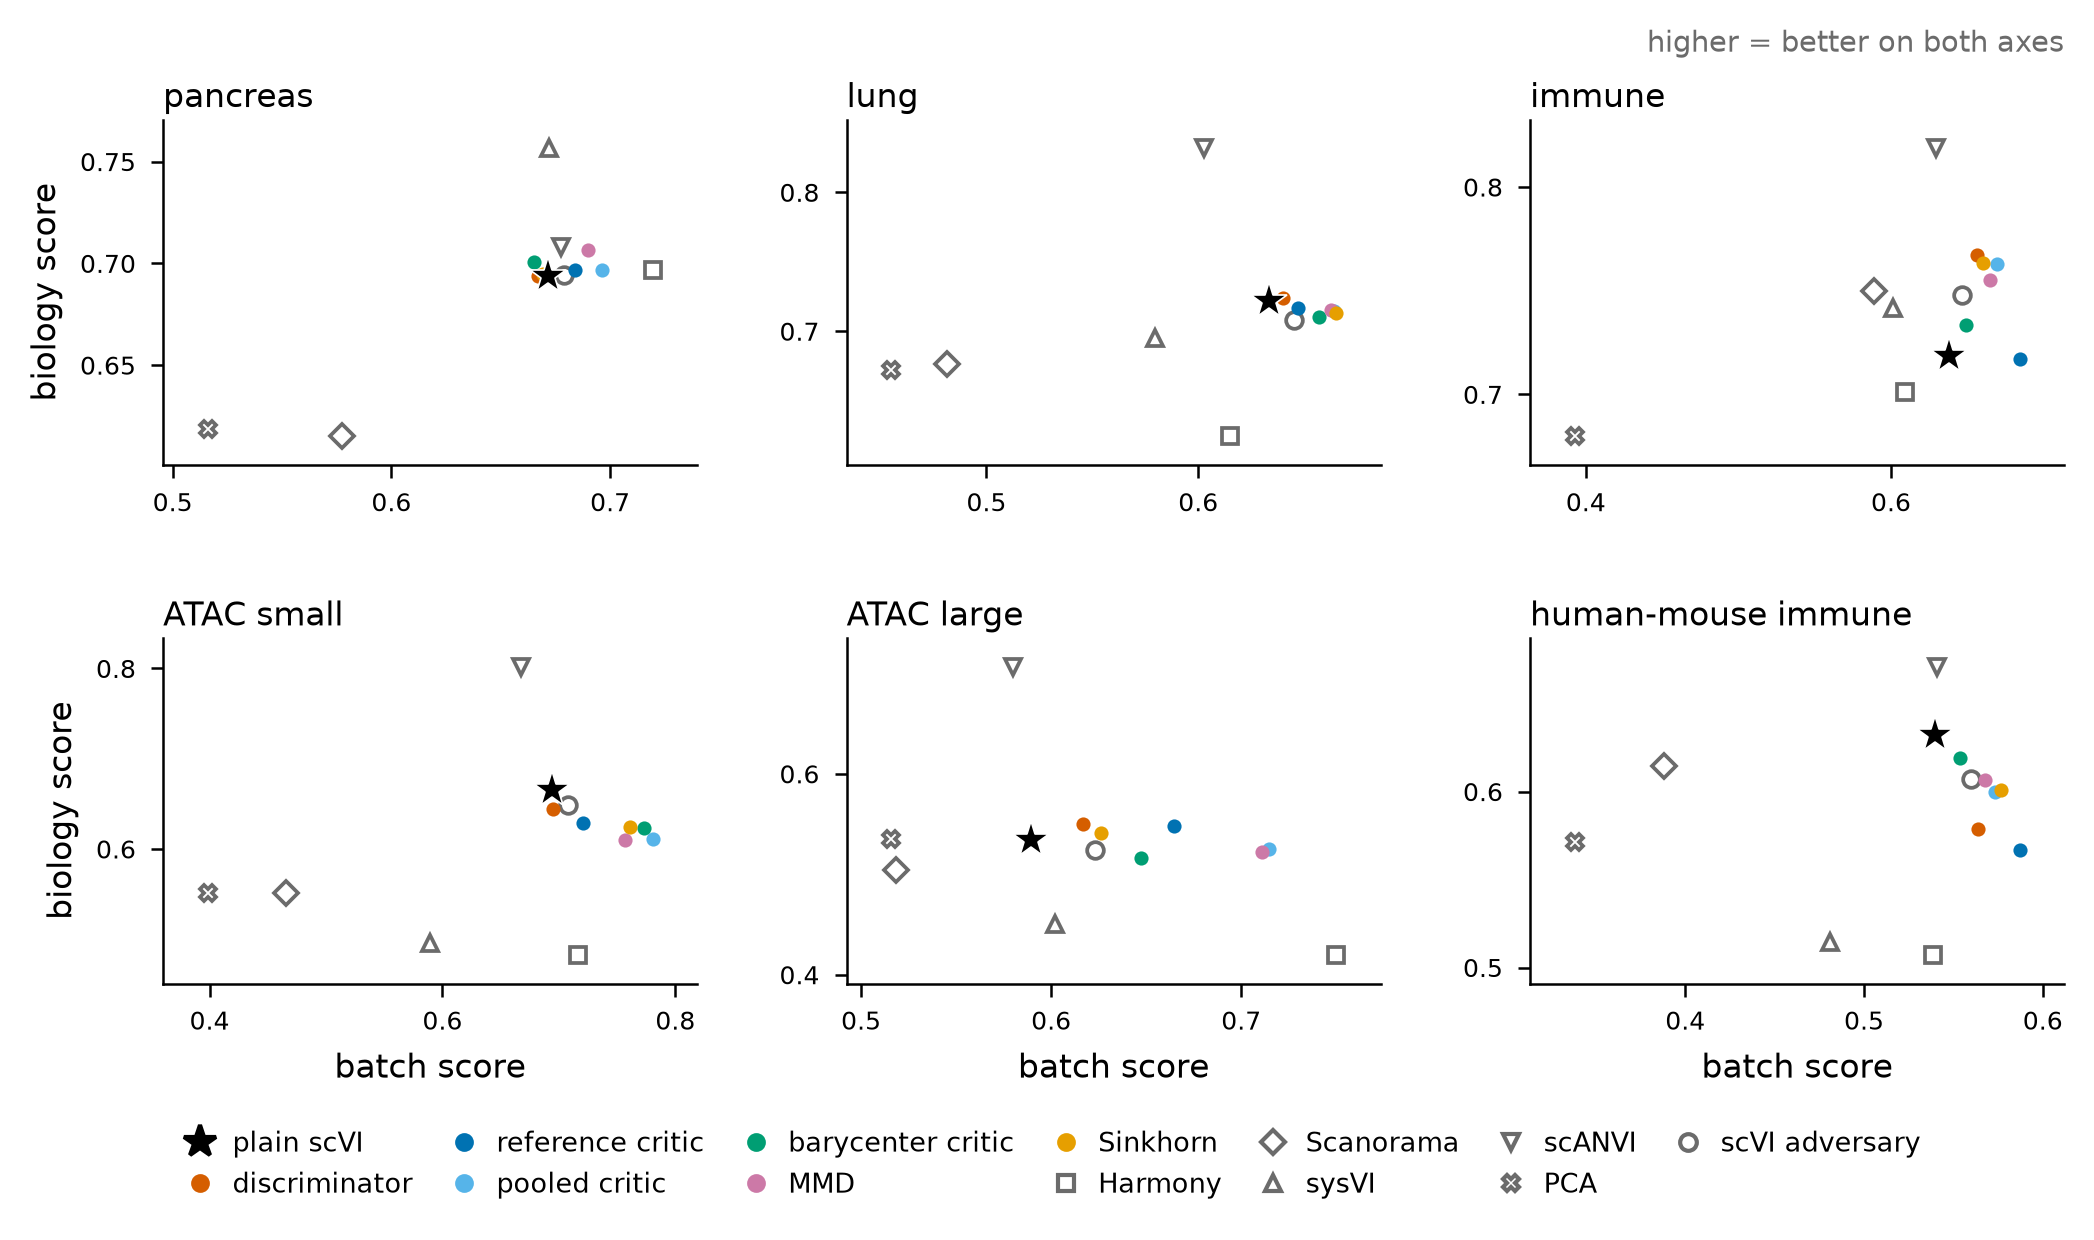
\includegraphics[width=\textwidth]{figures/fig5.png}
\caption{Collapse rate per penalty up to the highest common batch score, with the batch-conditioned decoder (a) and the unconditioned decoder (b): the percentage of a penalty's fits, at strengths whose mean batch score is at most the highest batch score every penalty reaches, that lose 0.10 or more biology against the same seed's plain scVI (lower is better; rates over all strengths in Supplementary Table S8). One point per real task, in the order of Figure 2a from top to bottom within each row, with its nominal exact 95\% interval; black tick, median over  the six real tasks, including the low-signal immune pair with the batch-conditioned decoder (ringed).}
\label{fig:5}
\end{figure}


\pp{Res-5}{Label transfer and a direct biology check read biology per cell type (Supplementary Figure S3 and Supplementary Table S10).}
Label transfer predicts the cell types of each held-out batch from the other batches, on each penalty's embedding at the strength nearest $b^*$ (Methods; Supplementary Note 9). With the unconditioned decoder, the discriminator's macro F1 was below plain scVI's on all six real tasks (median difference $-0.060$) and the lowest of the six penalties on each; with the batch-conditioned decoder it placed from first to last over the five ranked tasks (median difference $-0.006$). The other penalties' median differences from plain scVI were between $-0.016$ and +0.001 with either decoder (Supplementary Figure S3). Within a task, the penalties' label-transfer order did not follow their biology order at $b^*$ (Kendall $\tau_b$ median 0.067, range $-0.867$ to 0.600 over the 11 ranked pairs). The label-transfer embeddings lay at most 0.026 from $b^*$ in batch score (median 0.004), so they were not exactly matched. Along the full strength curves, label transfer also deteriorated at some strong settings: the barycenter critic ended at 0.360 on lung with the batch-conditioned decoder. The direct biology check is exploratory and descriptive: it was defined after the sweep scores had been read, uses 783 saved fits (penalties at the label-transfer strength, seeds 100--102; plain scVI; every scored baseline setting) and runs no test (Methods; Supplementary Note 12). Over the six real tasks, neighbourhood purity per cell type differed from plain scVI with the same decoder and seed by $-0.052$ for the discriminator with the batch-conditioned decoder and $-0.077$ with the unconditioned decoder, and by $-0.022$ and $-0.033$ for the Sinkhorn divergence; the reference, pooled and barycenter critics and MMD stayed between $-0.019$ and $+0.001$ with either decoder. Harmony, averaged over its 7 settings, differed from batch-conditioned plain scVI by $-0.141$, and scANVI, which is trained with the labels, by $+0.115$. Rare types (present on the pancreas, lung, immune and human--mouse immune tasks) lost purity in 23 of 48 task, penalty and decoder cells, most with the discriminator ($-0.107$ with the batch-conditioned decoder). The largest drop, $-0.406$, was for the 46 ionocytes of the lung task with the batch-conditioned discriminator at strength 3,000: their label-transfer recall was 0.326 (seed SD 0.407) against 0.797 for plain scVI, and a share of 0.232 of them was predicted as dendritic cells. Over all cell types, label-transfer recall differed from plain scVI by $-0.040$ and $-0.085$ for the discriminator with the two decoders and by $-0.024$ to $+0.003$ for the reference, pooled and barycenter critics and MMD. Marker genes were kept alike: the Jaccard overlap of the top 20 markers was 0.390 to 0.399 for every penalty and plain scVI, with differences from plain scVI of at most 0.006, whereas Harmony ($-0.031$) and PCA ($-0.028$) were lower. The direct readouts single out the discriminator, which also had the worst mean rank with the batch-conditioned decoder and the lowest label transfer on every real task with the unconditioned decoder (above); with the batch-conditioned decoder its loss of purity was larger for rare types than over all types.


% ---------------------------------------------------------------- Figure 5 (good-strength width; removed in Pass 23)
\noindent
%\begin{figure}[!htbp]
%\centering
%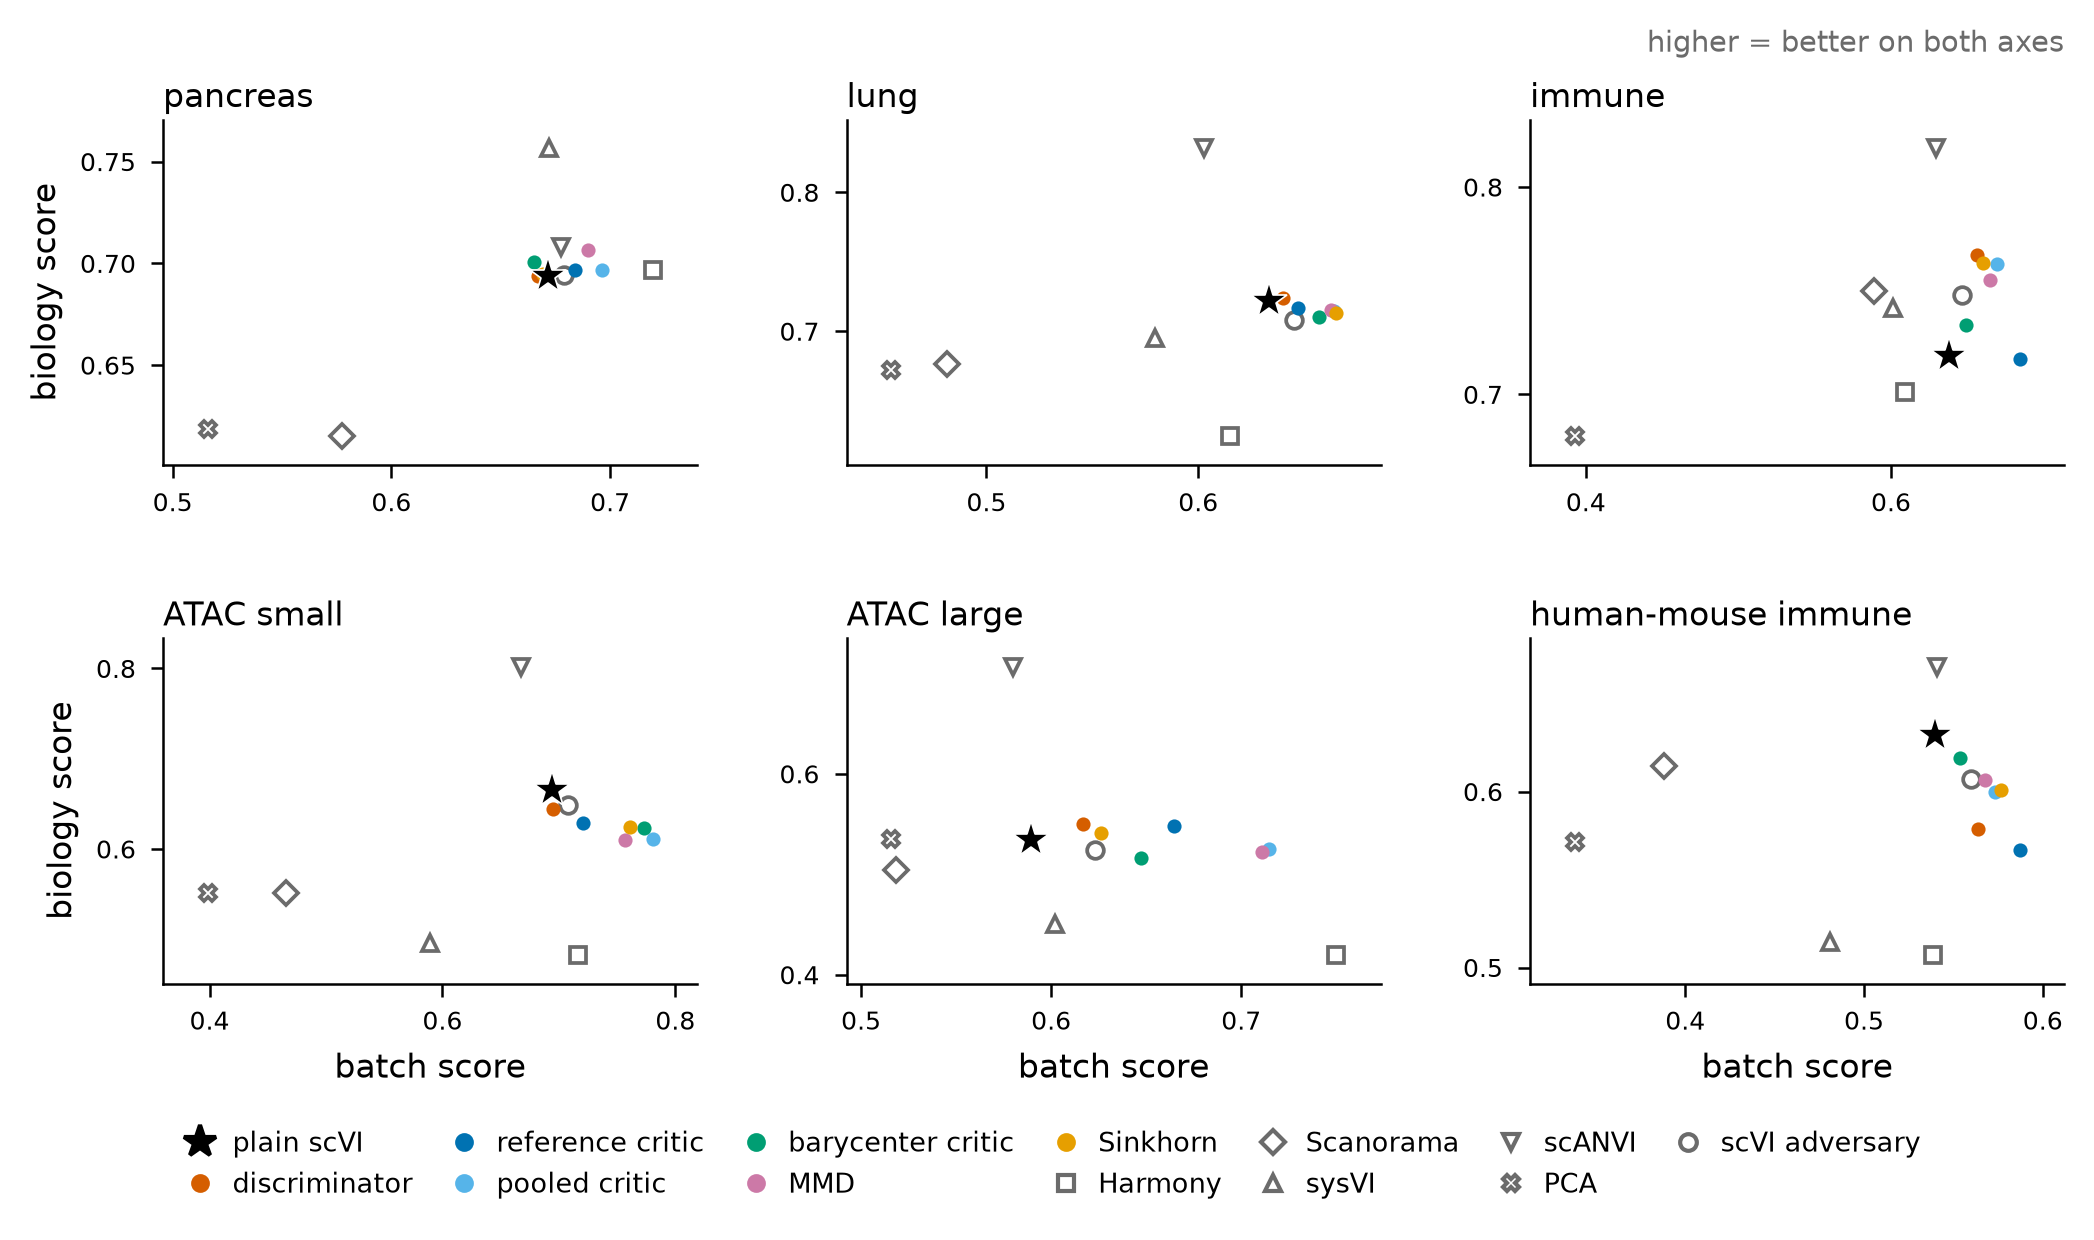
\includegraphics[width=\textwidth]{figures/fig5.png}
%\caption{Width of each penalty's range of good strengths, in decades, one point per real task and decoder (batch-conditioned decoder, circles, upper row of each band; unconditioned decoder, squares, lower row; tasks in the order of Figure \replaced[id=P23]{2a}{3} from top to bottom; black tick, mean over tasks). A good strength has a mean selection score at least the lower 95\% confidence bound of the best strength; a width of zero means a single qualifying strength. Ringed point, the low-signal immune pair with the batch-conditioned decoder, included as in the Results text.}
%\label{fig:5}
%\end{figure}
\pp{Res-6}{Single-strength tables place each method against plain scVI and the standard tools (Figure 6b; Supplementary Table \ref{tab:4}).}
\begin{itemize}
\item Rule: each penalty, and each of Harmony, Scanorama and sysVI at one of its settings, is shown at a strength or setting not tuned on that task, the one with the best mean selection score on real tasks of other families (related tasks never choose for each other), beside the task's own best strength as an optimistic bound; descriptive (Supplementary Notes 7 and 8, Table S4).
\item At the strength chosen on real tasks of other families, the penalties with the batch-conditioned decoder exceeded plain scVI's selection score on 3 (discriminator), 4 (reference critic), 5 (pooled critic), 5 (barycenter critic), 4 (MMD), 4 (Sinkhorn divergence) of the six real tasks, with differences from plain scVI from $-0.023$ to $+0.045$ (median $+0.006$; Supplementary Table \ref{tab:4}); 11 of these 36 differences were smaller than 0.005 in size (for example $-0.0004$ for the Sinkhorn divergence on pancreas, which Supplementary Table \ref{tab:4} prints as a tie), against seed standard deviations of the penalty's selection score of 0.001 to 0.016 in those cells, so the counts mix small gains, small losses and near-ties; at each task's own best strength, the optimistic bound, they did so on 5 to 6 of six. At their transferred settings, Harmony, Scanorama and sysVI exceeded batch-conditioned plain scVI on 1, 0 and 1 of six real tasks. With the unconditioned decoder, whose plain scVI receives no batch information, the penalties at the transferred strength exceeded plain scVI on 2 to 6 of six (Supplementary Table S7). The transferred strengths with the batch-conditioned decoder were discriminator 0.1--0.3; reference critic 0.3--3; pooled critic 1; barycenter critic 0.3--3; MMD 30; Sinkhorn divergence 1--100.
\end{itemize}

% ---------------------------------------------------------------- Figure 6
\begin{figure}[!htbp]
\centering
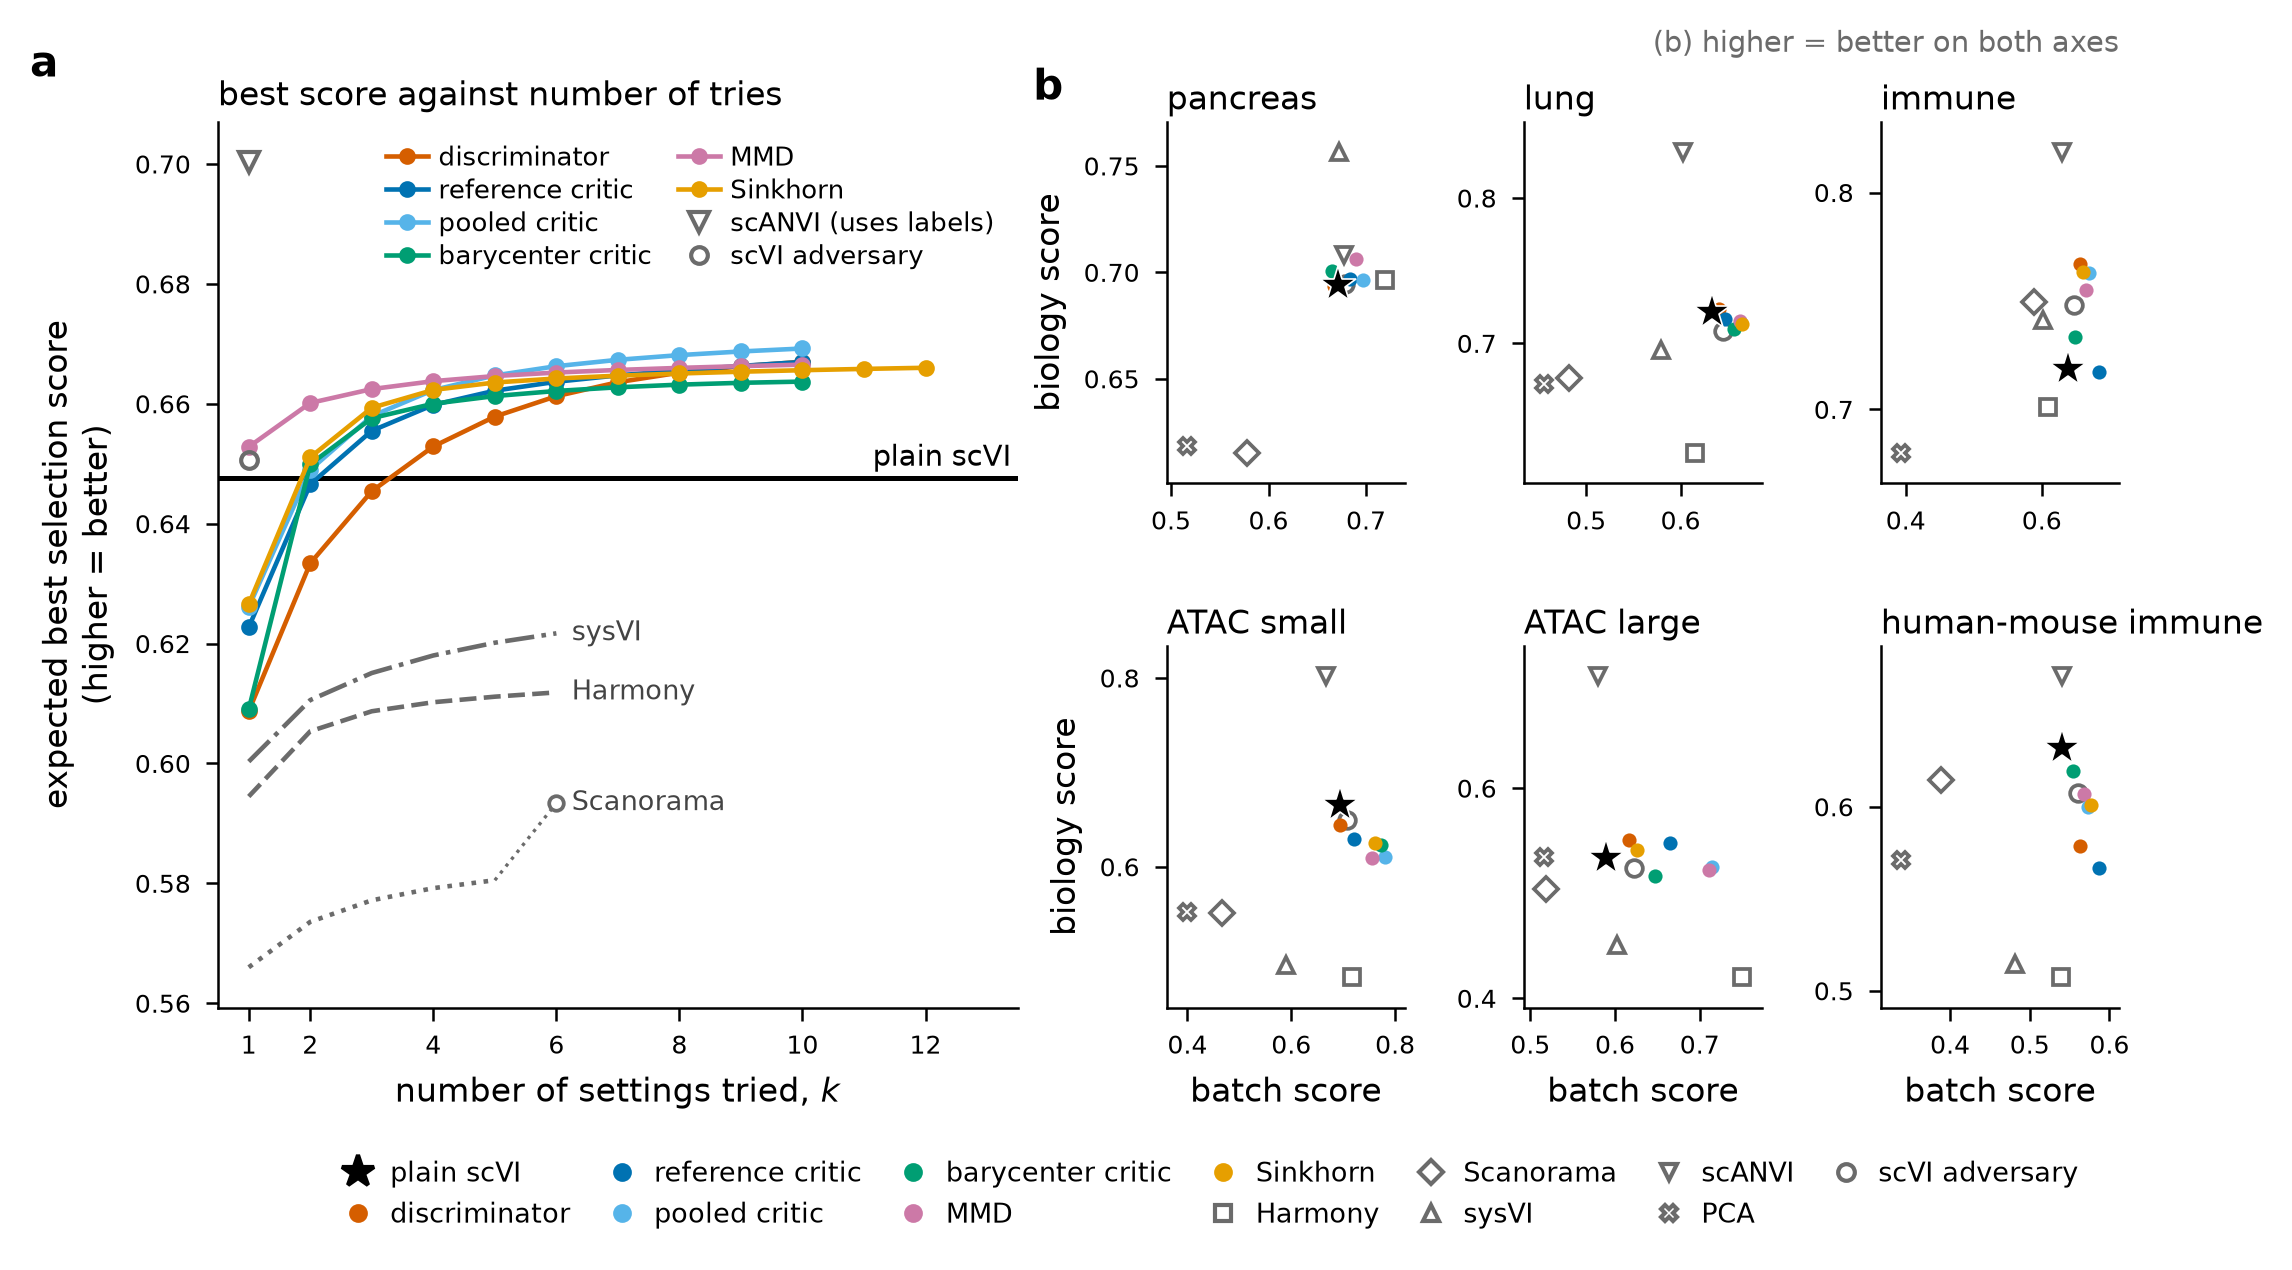
\includegraphics[width=\textwidth]{figures/fig6.png}
\caption{Placement against plain scVI and standard tools with the batch-conditioned decoder. (a) Expected best selection score among $k$ settings drawn at random, mean over the six real tasks of each method's per-task curve (Supplementary Figure S6; selection score: 0.4 batch plus 0.6 biology; optimistic, because the best setting is chosen and scored on the same data). Each curve is drawn up to the largest $k$ for which all six tasks have $k$ settings: $k=10$ for five penalties (the discriminator, reference critic and pooled critic have an eleventh setting on the immune task only) and $k=12$ for the Sinkhorn divergence, and $k=6$ for Harmony and sysVI. Scanorama has six settings on five tasks and five on the large chromatin-accessibility task (80 neighbours could not be fitted); it is drawn to $k=5$, and its $k=6$ value (open marker) is the mean of five tasks. The Results compare methods at $k=1$ and $k=6$, the number of settings of Harmony, Scanorama and sysVI; the penalty curves beyond $k=6$ are shown for completeness. Horizontal line, plain scVI (0.648); scANVI (uses cell-type labels) and the scVI adversary have one setting. At $k=1$ every penalty except MMD scored below plain scVI; the other penalties first exceeded plain scVI at $k=2$ (pooled critic, barycenter critic, Sinkhorn divergence), 3 (reference critic) and 4 (discriminator). (b) Batch against biology score for each real task at the single strength (penalties, Harmony, Scanorama, sysVI) chosen on other task families, or at the fixed setting (scANVI, scVI adversary, PCA with 10 dimensions); star, plain scVI. The unconditioned decoder is in Supplementary Table S7.}
\label{fig:6}
\end{figure}

\pp{Res-7}{The comparison at equal numbers of tries reports whether any penalty improves on plain scVI (Figure 6a; per-task curves in Supplementary Figure S6).}
\begin{itemize}
\item Rule: each method gets the expected best selection score among $k$ of its settings drawn at random, $k=1$--6, the number of settings of Harmony, Scanorama and sysVI (comparisons at equal tries stop at six, although the penalties have ten or twelve sweep strengths), so methods with more settings gain no advantage; optimistic because the best setting is chosen and scored on the same data; scANVI has its own stratum (Supplementary Note 7).
\item With the batch-conditioned decoder, a penalty's expected best selection score at one try exceeded plain scVI's on 0, 2, 2, 0, 3, 1 of the six real tasks (in the order discriminator, reference, pooled and barycenter critics, MMD, Sinkhorn divergence), 8 of 36 task--penalty cells, and at six tries on 4, 5, 5, 5, 5, 6 (30 of 36). Averaged over the six real tasks, plain scVI scored 0.648; the penalties ranged from 0.609 to 0.653 at one try and from 0.661 to 0.666 at six (Figure 6a), and their real-task means first exceeded plain scVI's at 4, 3, 2, 2, 1, 2 tries in the same order. Against the standard tools at six tries, every penalty exceeded Harmony on 5 of six real tasks, sysVI on 5 of six and Scanorama on all 5 tasks where its six settings exist; at one try the counts were Harmony 4 to 5, sysVI 4 to 5 and Scanorama 6 of six. The scvi-tools adversary (mean 0.651) was exceeded at one try on 0 to 4 of six tasks and at six tries on 5 to 6. scANVI, which uses the cell-type labels (mean 0.700), was exceeded by no penalty at one try with either decoder; at six tries with the batch-conditioned decoder every penalty exceeded it on pancreas only, by 0.002 to 0.010, and with the unconditioned decoder on no task. With the unconditioned decoder the reference is plain scVI without batch information (mean 0.578), which the penalties exceeded at one try on 1 to 5 of six real tasks and at six tries on 5 to 6. Every best-of-$k$ value is optimistic for methods with more than one setting, because the best setting is picked and scored on the same data (Supplementary Note 7).
\end{itemize}

\hd{Discussion}{700 words; 5 paragraphs}
\pp{Disc-1}{The penalty with the best mean rank depended on the decoder: the pooled critic with the batch-conditioned decoder, closely followed by the Sinkhorn divergence, and MMD with the unconditioned decoder. Task-level orders varied, and many neighbouring biology readings were within a leave-one-seed-out standard error, so these descriptive rankings do not establish a consistent ordering across tasks. The secondary summaries gave different orders again: MMD had relatively low collapse rates despite ranking near the bottom with the batch-conditioned decoder. This exploratory comparison on eight tasks with three seeds (100--102) supports a decoder-specific description of the sweep; the replication across training seeds, on new seeds of the same tasks, kept the four large within-pair gaps and agreed with the pair orders in part, but the leaders changed: on the new seeds the Sinkhorn divergence had the best mean rank with the batch-conditioned decoder and the pooled critic with the unconditioned decoder, while the discriminator stayed last with the batch-conditioned decoder (Res-2b; Supplementary Note 13).}
\begin{itemize}
\item The replication across training seeds met its agreement rule: the four large within-pair gaps kept their sign, and the sweep and replication orders were positively correlated (mean $\tau_b$ 0.456, $p=0.00049$; $p=0.0039$ with signs flipped per task and $p=0.0156$ per task family; all three values are approximate, because related tasks are not independent). The orders did not hold in detail: the first-ranked penalty changed in 7 of 13 pairs, $\tau_b$ was slightly negative in 2 pairs (pancreas and the human--mouse immune task, both with the batch-conditioned decoder; $\tau_b=-0.067$), and MMD on pancreas with the batch-conditioned decoder did not replicate its crossing. The replication therefore supports the large gaps and the broad order, not the order of near-tied penalties (its limits are in Disc-4).
\end{itemize}
\pp{Disc-2}{The secondary analyses suggest that the penalties differ partly in how much biology they lose as strength increases. The discriminator often lost biology beyond the matched level, while MMD generally had lower collapse rates, yet lower collapse did not ensure a higher biology rank at $b^*$. Hypervolume and the share of non-dominated strengths describe other aspects of the curves, so their orders need not agree with a ranking at a single batch score. Label-transfer scores did not follow the matched-biology ranking either, and their batch-score distances from $b^*$ limit direct comparisons.  These patterns describe each penalty as it is usually trained, with each adversary's update steps and optimiser at its standard setting (Methods).}
\pp{Disc-3}{For users of scVI, the sweep points to the penalty strength, more than the choice among penalties, as the setting that matters. At matched batch removal the six penalties were near-tied: 160 of the 195 within-pair differences in biology over the 13 ranked pairs were under 0.02, and 4 were 0.04 or more. With the batch-conditioned decoder, going from one to six tries raised each penalty's mean expected best selection score over the real tasks by 0.012 to 0.053, whereas at six tries the six penalties' means spanned only 0.661 to 0.666. Added to scVI as it is usually run, with the batch-conditioned decoder, a penalty at one strength drawn at random rarely beat plain scVI (8 of 36 task--penalty cells); the best of six strengths did in 30 of 36, by small margins (real-task means 0.661--0.666 against 0.648).}
\begin{itemize}
\item When to add a penalty: when several strengths can be fitted and scored on the task, because the real-task mean of the best of $k$ first exceeded batch-conditioned plain scVI at 1 (MMD) to 4 (discriminator) tries. Strength range: the strengths chosen on other task families with the batch-conditioned decoder lay between 0.1 and 100. Standard tools: at equal tries the penalties exceeded Harmony, Scanorama and sysVI on most real tasks, but not scANVI, which uses cell-type labels and was exceeded only on pancreas at six tries. These are optimistic best-of-$k$ readings on eight scIB tasks.
\end{itemize}
\pp{Disc-4}{The design limits what the data can show.}
\begin{itemize}
\item  Six real tasks in four families, two of them nested pairs (human--mouse immune contains all immune cells; large ATAC contains small); related tasks count as separate tasks in the mean rank, and the ranking is descriptive. A penalty whose curve does not reach $b^*$ is ranked last in that pair, so a missing reading counts as the worst result.
\item The comparison is exploratory. The strength grid was fixed in advance and the sweep reports all ten strengths (the strengths of the single-strength tables and of the replication were then chosen from sweep scores, as Methods describes); the planned fixed-strength benchmark  (six strengths per family, five new seeds) was replaced by the smaller replication across training seeds. The sweep results  test no hypothesis fixed in advance, and the ranking rules were applied to the same fits that the strength-choice rules had already read. With three seeds per strength, the standard errors in Supplementary Table S6 show how far apart neighbouring ranks are. The replication checks the sweep's readings at $b^*$ on new fits against a prediction and an agreement rule fixed before any replication score was read, but it refits the same eight tasks with new training seeds, not new data, so it says nothing about other datasets, batch structures or preprocessing. Its rule tests only the sign of the within-pair differences of 0.04 or more, and no precision calculation was made, so it does not separate penalties whose readings differ by less. Its strengths and $b^*$ were set from the sweep's batch scores after the sweep had been read, so it replicates the sweep's readings rather than testing a hypothesis fixed before the sweep.
% Pass 8: the next bullet (Pass 7 text, shown struck through) describes standard settings, not a limitation, and is moved to the Methods paragraph on the fixed backbone.
% Pass 7 replaced this earlier wording: Regularisation (gradient penalty, spectral normalisation) and the number of adversary update steps were not varied: the reference, pooled and barycenter critics take five steps per encoder step and the discriminator one, so a difference between penalties includes these settings and is not due to the divergence alone.

\item All fits use one backbone, scVI, with one fixed architecture and latent size (10 latent dimensions, one hidden layer of 128 units), so the ranking may not hold for other backbones, architectures or latent sizes. The eight tasks are of the size of the single-cell integration benchmark, not of an atlas, so the ranking may not hold for integrations at atlas scale.  The biology checks, including label transfer, are exploratory: they were defined after the sweep scores had been read.
\item The strength sweep is what Li et al.\ call scalarization: one penalty is run at a series of fixed strengths and both scores are read at each \citep{li2022trade}. The ranking therefore describes the penalties as users run them, not the best trade-off front that a multi-objective solver could reach for each penalty. Li et al.\ also used an adversarially trained mutual-information penalty (MINE); it is not among the six penalties and was not tested here.
\item One batch variable per task; ATAC as gene-activity matrices; non-integer counts as distributed; scoring includes training cells; Sinkhorn not W1; reference choice uses labels.
\item The collapse-rate intervals are nominal exact binomial 95\% intervals. They treat a penalty's fits in a task and decoder (6 to 33 up to the highest common batch score; over all strengths 30, 33 for the discriminator, the reference critic and the pooled critic on the immune task with the batch-conditioned decoder, which have additional strengths, and 36 where edge strengths were fitted) as independent, although each seed's fits are judged against the same plain-scVI threshold and can collapse together, so their actual coverage may differ from 95\%. An illustrative simulation of this dependence is in Supplementary Note 7; it covers only 30 and 36 fits and does not bound the coverage of the intervals reported here.
\end{itemize}
\pp{Disc-5}{Several factors are outside the scope of this comparison.}
\begin{itemize}
\item Not varied or tested: architecture, Kullback--Leibler (KL) warm-up (incomplete on shorter tasks, penalty from start), reference batch, batch number; composition shift read from strength curves, not a dose-response test.
\end{itemize}

\hd{Conclusions}{about 150 words; 1 paragraph}
\begin{itemize}
\item On eight tasks of the single-cell integration benchmark, six alignment penalties added to one scVI model kept similar biology at matched batch removal: the best mean rank was the pooled critic's with the batch-conditioned decoder (2.20) and MMD's with the unconditioned decoder (2.17), but 160 of the 195 within-pair differences were under 0.02, so the ranking does not separate most penalties, and on new training seeds the Sinkhorn divergence and the pooled critic led instead. At equal numbers of tries with the batch-conditioned decoder, the penalties exceeded Harmony, Scanorama and sysVI on most real tasks and plain scVI mainly when several strengths were tried and scored on the same data; scANVI, which uses cell-type labels, was exceeded only on pancreas.
\item Observations for scVI users, from the scores on these eight tasks and not tested on independent data: (i) the strength mattered more than the choice of penalty, and plain scVI with the batch-conditioned decoder remained a strong candidate, since a penalty at one strength drawn at random beat it in 8 of 36 task--penalty cells and the best of six strengths in 30, a count that is optimistic because the strengths were chosen and scored on the same data; (ii) the strengths chosen on other task families with that decoder lay between 0.1 and 100 across penalties (Results); (iii) the biology was worth checking directly at the chosen strength, because the discriminator lost the most neighbourhood purity in the direct biology check ($-0.052$ against plain scVI, $-0.107$ for rare types, batch-conditioned decoder); (iv) when cell-type labels were available, scANVI scored higher than every penalty on most tasks, but it is trained with the labels that several biology metrics also use, so its biology scores are not label-free.
\end{itemize}

\hd{Declarations}{eight BMC subheadings, each filled or marked not applicable}
\pp{Ethics approval and consent to participate}{Not applicable. This study analyses only publicly available, previously published data: the integration tasks of the single-cell integration benchmark (figshare article 12420968, version 8), which hold human and mouse single-cell data from earlier studies, and two simulated datasets. No new data were collected from human participants or animals.}
\pp{Consent for publication}{Not applicable.}
\pp{Availability of data and materials}{Code and data access.}
\begin{itemize}
\item Repository github.com/kreid415/wasserstein-critic-deconfounding; fitting and scoring code at commit 10a1ca5, sweep analysis at commit 8595a16, biology check at commit c4a793f, figure scripts and their inputs in \texttt{paper/figure\_scripts} and \texttt{paper/figure\_data}; \tbd{release tag and commit of the submitted version}; checksums in supplement.
\item The eight task files are the integration-task datasets of the single-cell integration benchmark, figshare article 12420968, version 8 (doi:10.6084/m9.figshare.12420968.v8); file checksums in Supplementary Table S1.
\end{itemize}
\pp{Competing interests}{The authors declare that they have no competing interests.}
\pp{Funding}{\tbd{funding statement}}
\pp{Authors' contributions}{\tbd{authors' contributions statement}}
\pp{Acknowledgements}{\tbd{acknowledgements}}
\pp{Authors' information (optional)}{Not applicable.}

\hd{Supplementary material}{Supplementary Notes 1--13, Tables S1, S2 and S4--S14, Figures S1--S7}
\noindent Every supplementary note and table listed here is in this document: Supplementary Notes 2--13 and Tables S1, S2, S4, S5 and S8 are printed below in the place of their entries (Table S11 within Note 9); Table S10, then Supplementary Note 1, Tables S6, S7, S9 and S12--S14 and Figures S1--S7, follow the main figures. Table S3 (strength ranges of the planned fixed-strength benchmark) was removed with that benchmark, and its number is not used.\par
% Pass 17: the supplementary tables input in this list step the table counter; it is restored after the list (main tables 1-3)
\newcounter{maintables}\setcounter{maintables}{\value{table}}\let\mainTheHtable\theHtable\renewcommand{\theHtable}{supp.\arabic{table}}%
\Needspace{5\baselineskip}\textbf{Supplementary Notes}
\begin{itemize}
\item Supplementary Note 1, model and loss equations: notation, with the reconstruction term written per gene $g$ as $p_{\mathrm{ZINB}}(x_g \mid \mu_g, \theta_g, \pi_g)$ (mean, dispersion, dropout) and the discriminator loss as $\min_{h}\, \frac{1}{|\mathcal{B}|}\sum_{i\in\mathcal{B}}\mathcal{L}_{\mathrm{CE}}(h(u_i), s_i)$ on the posterior mean $u_i=\mu_i$ of cell $i$ in minibatch $\mathcal{B}$, for batch label $s_i$; scVI loss (zero-inflated negative binomial reconstruction, Kullback--Leibler (KL) term and KL weight schedule); discriminator fool loss as in scvi-tools (Jensen--Shannon type); the three Wasserstein-1 critics with gradient penalty weight 10: reference (each batch against the reference batch, chosen as the batch with the highest cell-type entropy, which uses labels), pooled (each batch against all others), barycenter (each batch against the minibatch Wasserstein barycenter, an average distribution); barycenter target construction and solver (Wasserstein-2, at most 10 iterations, threshold $10^{-7}$); maximum mean discrepancy (MMD) with multi-scale Gaussian kernel (the squared MMD of each batch against the cells of all other batches in the minibatch, as a biased V-statistic, averaged over the batches present; the kernel is the mean of five Gaussian kernels $\exp(-\lVert z-z'\rVert^2/2\sigma^2)$ with $\sigma=\sqrt{d}\,m$ for $m\in\{0.25,0.5,1,2,4\}$, so for $d=10$ latent dimensions the bandwidths are $\sigma=0.79$, $1.58$, $3.16$, $6.32$ and $12.65$; they are fixed in advance and not tuned, and the MMD results hold for this kernel); debiased Sinkhorn divergence (entropy-regularised optimal transport; not W1 at the smoothing used; Euclidean cost, entropic smoothing $0.05\sqrt{2d}$ for latent dimension $d$, float64, marginal error $10^{-4}$, cap of 500,000 iterations); scvi-tools adversarial classifier (conditioned decoder only; 32 hidden units, weight one minus the KL weight); plain scVI as strength zero; each critic head has two hidden layers of 128 units with one output per batch.
\end{itemize}
\Needspace{5\baselineskip}\medskip\noindent\textbf{Supplementary Note 2. Training settings.}\par\smallskip
\begingroup\small\setlength{\parskip}{3pt}
Plain scVI, the six penalties and the scvi-tools adversary share the scVI backbone and task settings in Supplementary Table S2. The model has 10 latent dimensions and one hidden layer of 128 units in each network. It uses a zero-inflated negative binomial likelihood, a 90\% training split and minibatches of 128 cells. The encoder and decoder use Adam with learning rate $10^{-3}$, epsilon 0.01 and weight decay $10^{-6}$.

The discriminator uses the same optimiser settings and one adversary update per encoder step. Wasserstein critics use five updates, gradient-penalty weight 10 and Adam with learning rate $10^{-4}$ and betas 0 and 0.9. These are each method's standard settings. MMD and Sinkhorn have no adversary network. Adversary updates reuse detached posterior means from one minibatch, followed by an encoder update on that minibatch.

Two input pilots compared posterior samples with means for the discriminator and reference and pooled critics, and standardised with unstandardised means for those methods, MMD and Sinkhorn. Standardisation used each dimension's minibatch mean and standard deviation. Both used the immune and small chromatin-accessibility tasks, both decoders, seeds 100--102 and three strengths around matched batch removal. A comparison was evaluable if both curves reached $b^*$. Switching required at least two-thirds of comparisons evaluable, with one in every task--decoder pair. It also required the mean biology difference at $b^*$ (alternative minus default) to exceed 0.01 and to be positive within every pair, and no more failed fits. Posterior samples gave mean improvement $-0.004$ with 9 of 12 comparisons evaluable. Standardisation gave $-0.003$ with 14 of 20 evaluable. Neither met the switching criteria, so posterior means without standardisation were retained.

Training lasts $\min(400,\mathrm{round}(20000\times400/n))$ epochs for $n$ cells, without early stopping. The KL weight rises over 400 epochs, reaching $(E-1)/400$ in the last of $E$ epochs. Shorter tasks therefore finish before warm-up is complete. The penalty remains at full strength throughout. A fit fails if any computed or back-propagated loss term, or any posterior-mean latent value, becomes non-finite.

A seed fixes scVI initialisation and the training split across methods. Minibatch order matches within a method and between plain scVI, MMD and Sinkhorn. Constructing an adversary consumes random draws before training, so its minibatch order can differ.
\par\endgroup
\par
\Needspace{5\baselineskip}\medskip\noindent\textbf{Supplementary Note 3. Data preparation and scIB scores.}\par\smallskip
\begingroup\small\setlength{\parskip}{3pt}
The eight tasks come from scIB, figshare article 12420968, version 8 (Supplementary Table S1). All cells are retained. RNA tasks use scIB's batch and cell-type variables and 2,000 highly variable genes selected batch-wise with cell-ranger flavour and 20 bins on normalised expression. Chromatin-accessibility tasks use their supplied labels and all 3,429 or 3,580 gene-activity features. Counts are used as distributed, including non-integer values in 18 batches. These comprise transcripts per million in the Villani batch of both immune tasks, reads per kilobase per million, expected counts and collision-corrected counts in the pancreas batches smarter, fluidigmc1, celseq and celseq2, and normalised values in the twelve 10x batches of lung.

scib 1.1.7 scores posterior means for all cells, including training cells. Metrics retain their raw scales, with higher values better. The batch score $B$ averages five batch metrics. The biology score $C$ averages the applicable biology metrics, and $S=0.4B+0.6C$ is the selection score. Unlike scIB's overall score, these means use no scaling across methods. Let $K$ denote batches, $L$ cell types and $G_{15}$ the embedding's 15-nearest-neighbour graph.

\noindent\textit{Batch metrics.} Principal-component regression is $\mathrm{PCR}=\sum_j R_j^2V_j/\sum_jV_j$, where $R_j^2$ measures batch association and $V_j$ component variance. It uses 50 components of unintegrated normalised expression on all genes and all embedding dimensions. Its score is $\max\{0,(\mathrm{PCR}_{\mathrm{before}}-\mathrm{PCR}_{\mathrm{after}})/\mathrm{PCR}_{\mathrm{before}}\}$.

Batch average silhouette width (ASW) averages $1-|a_i|$ within cell types spanning multiple batches, then across types. Silhouettes use Euclidean distances and batch clusters. Graph iLISI uses 90 shortest-path neighbours on $G_{15}$, weighted at perplexity 30, for a random subsample of about half the cells. With median inverse Simpson index $m$, its score is $(m-1)/(K-1)$. Graph connectivity averages, over cell types, the fraction of a type's cells in the largest connected component of $G_{15}$ restricted to that type.

kBET uses a 50-nearest-neighbour graph and tests types with at least 10 cells spanning multiple batches. Its $\chi^2$ test compares diffusion-neighbour batch composition with the type's composition, using $k_0=\min\{70,\max(10,\lfloor\bar n_c/4\rfloor)\}$, where $\bar n_c$ is mean cells per batch. Disconnected components smaller than $3k_0$ are dropped if at least 75\% of cells remain. Otherwise the rejection rate is 1. The score is one minus mean rejection rate across tested types. R's seed is 0 for each call.

\noindent\textit{Biology metrics.} Leiden clustering of $G_{15}$ uses resolutions $0.2,0.4,\dots,2.0$. The clustering $\kappa$ maximising cell-type normalised mutual information is retained, with $\mathrm{NMI}=2I(\kappa;c)/(H(\kappa)+H(c))$. Its adjusted Rand index is $\big(\sum_{uv}\binom{n_{uv}}2-\Sigma_{ab}\big)/\big(\tfrac12[\sum_u\binom{a_u}2+\sum_v\binom{b_v}2]-\Sigma_{ab}\big)$, where $n_{uv}$ counts cluster--type intersections, $a_u,b_v$ are margins and $\Sigma_{ab}=\sum_u\binom{a_u}2\sum_v\binom{b_v}2/\binom n2$.

Cell-type ASW is $(\bar a+1)/2$, using mean Euclidean silhouette by cell type. Isolated labels occur in the fewest batches, unless every type occurs in every batch. Isolated-label F1 averages each label's best F1 over clusters and resolutions. Isolated-label ASW averages $(\bar a_\ell+1)/2$ over those labels, where $\bar a_\ell$ is the mean cell-type silhouette within a label. Graph cLISI uses iLISI neighbourhoods with cell-type labels and score $(L-m)/(L-1)$.

Cell-cycle conservation applies to pancreas, lung and both immune tasks. Human S and G2M gene scores give PCR variance contributions $v$ before and after integration within each batch. The score averages $\max\{0,1-|v_{\mathrm{after}}-v_{\mathrm{before}}|/v_{\mathrm{before}}\}$ across batches. Trajectory conservation applies to the immune tasks. Diffusion pseudotime is recomputed within the largest connected component, using a root chosen from supplied pseudotime and labels. Values above 1 and outside the component become 0. The score is $(\rho+1)/2$ for Spearman correlation with supplied pseudotime, or 0 without a root.

All tasks use the six metrics from NMI through cLISI. Pancreas and lung add cell-cycle conservation, giving seven metrics. Both immune tasks also add trajectory conservation, giving eight. Undefined metrics are omitted. Highly variable gene conservation is undefined for embeddings. All batch metrics are available. Scores lie between 0 and 1 except ARI, whose minimum was $-0.00003$.
\par\endgroup
\par
\Needspace{5\baselineskip}% Supplementary Note 4: penalty-strength sweep, design and coverage; replication across training seeds, design.
% Sources: run lists and records of the sweep analysis (D/sweep_analysis_final_20261105, commit 8595a16; paper/figure_data), docs/PREREG.md (history),
% fit ledgers under D/tier12_v3 and D/jhpce_tier12, experiments/sweep_replication/ (branch sweep-replication, a475ea3). Numbers: paper/supp-analysis_numbers.csv.
\par\medskip\noindent\textbf{Supplementary Note 4. Penalty-strength sweep: design and coverage.}\par\smallskip
\begingroup\small\setlength{\parskip}{3pt}
\noindent\textit{Design.} Plain scVI and the six penalties (Supplementary Note 1) were fitted on all eight tasks at the ten half-decade strengths 0.1, 0.3, 1, 3, 10, 30, 100, 300, 1,000 and 3,000, with the batch-conditioned and the unconditioned decoder and with seeds 100, 101 and 102. Edge strengths were added in two places: the discriminator with the unconditioned decoder was also fitted at 0.01 and 0.03, and the Sinkhorn divergence with the batch-conditioned decoder at 10,000 and 30,000. Each task therefore has 378 fits: 6 of plain scVI (three seeds, two decoders), 360 of the penalties (six penalties, ten strengths, three seeds, two decoders) and 12 at edge strengths (two places, two strengths, three seeds), so the sweep has 3,024 fits on the eight tasks, 96 of them at edge strengths. Nine further fits, at strength 0.03 for the discriminator, the reference critic and the pooled critic on the immune task with the batch-conditioned decoder (seeds 100--102), come from an earlier strength-extension round (below). The analysis reads every fitted strength, so it reads 3,033 fits, 387 of them on the immune task. A penalty's curve therefore has ten strengths, twelve for the discriminator with the unconditioned decoder and for the Sinkhorn divergence with the batch-conditioned decoder on every task, and 11 for the discriminator, the reference critic and the pooled critic on the immune task with the batch-conditioned decoder. None of the 3,033 fits failed (Supplementary Table S5).

\noindent\textit{Why the edge strengths exist.} The sweep was first run as a pilot on the three tasks fitted first (the small chromatin-accessibility, immune and simulation 1 tasks). A strength-choice rule, written before the pilot ran, was to read the pilot's seed means and set, for each penalty family and decoder, a range of six strengths for a planned fixed-strength benchmark; where a range reached the end of the grid, the rule asked for two more half-decade strengths beyond that end. On the three tasks this happened in two places, the discriminator with the unconditioned decoder at the low end and the Sinkhorn divergence with the batch-conditioned decoder at the high end, and the two extra strengths were fitted there (36 fits on the three tasks). When the sweep was extended to the other five tasks, the same 378 fits per task were made, the edge strengths included, so every task has the same strengths. The nine further fits come from a second rule, which matched batch removal at a strength nearest a target batch score and, where that strength was the lowest of its grid, fitted the next lower half-decade value; this happened for three penalties on the immune task with the batch-conditioned decoder. They are not strengths of the strength-choice rule, but they are fitted points of these penalties' curves and are read like every other strength. That pair is low-signal and is not ranked (Supplementary Note 5).

\noindent\textit{The planned fixed-strength benchmark was not run.} The strength-choice rules were written to set up a benchmark at six strengths per penalty family and decoder with five new seeds. That benchmark was not run, so the strength-choice rules choose no strength: every analysis reads every sweep strength, and the comparison is exploratory. The replication across training seeds (below) refits strengths chosen from the sweep's batch scores, not from its biology scores.

\noindent\textit{Machines.} All fits of a task were made on one kind of machine, so that the hardware never differs between penalties, strengths or decoders within a task: the small chromatin-accessibility, immune and simulation 1 tasks on the workstation's NVIDIA RTX 3080 graphics card, and each of the other five tasks in one cluster job on NVIDIA L40S graphics cards (Supplementary Note 11).

\noindent\textit{Sinkhorn solver.} All 528 Sinkhorn fits of the sweep (66 per task) were made with the corrected Sinkhorn solver, at commit 10a1ca5 (Supplementary Note 1 gives the solver). On the three workstation tasks, the fits made with the earlier solver were replaced: the 180 fits at the ten grid strengths were refitted on 17--18 October 2026 and the 18 fits at the edge strengths 10,000 and 30,000 on 19 October 2026, 198 in all. The five cluster tasks were fitted from 22 October 2026 at the same commit.

\noindent\textit{Replication across training seeds: design.} For each of the 13 ranked task and decoder pairs and each of the six penalties, we took the two sweep strengths that bracket the first crossing of $b^*$ on the sweep's seed-mean curve, with $b^*$ fixed at its sweep value (Supplementary Note 5), and refitted them with five new seeds (0--4). 46 of the 78 curves cross $b^*$ more than once; the first crossing sets the bracket, as in the sweep reading. In one cell, the discriminator with the batch-conditioned decoder on the human--mouse immune task, the curve already lies above $b^*$ at the lowest sweep strength, 0.1, so the bracket runs from plain scVI to that strength and plain scVI at the new seeds is its lower point. Plain scVI was refitted at seeds 0--4 on all eight tasks with both decoders. This gives 855 fits, 775 with a penalty and 80 of plain scVI. The three low-signal pairs (the immune task and both simulations with the batch-conditioned decoder) were skipped. If the new seed means at the two strengths do not bracket $b^*$, the next sweep strength outward is fitted once with seeds 0--4; if $b^*$ is still not bracketed, the penalty takes the bottom rank in that pair and is marked as not replicating the crossing. The fits of this extension step are counted in Supplementary Note 11, and the readings that needed it are marked in Supplementary Table S9.

\noindent\textit{Replication: provenance.} The design script \texttt{experiments/sweep\_replication/replication\_design.py} wrote the run list (\texttt{manifests/sweep\_replication\_x1.tsv}, 855 rows) and its summary in \texttt{experiments/sweep\_replication/design\_20261102/} (commit 2113ec7). The prediction file \texttt{PREDICTION.json} (the sweep readings and ranks at $b^*$ of the 13 ranked pairs and the 4 within-pair differences of 0.04 or more) and the agreement rule \texttt{AGREEMENT.md} were committed under the tag \texttt{replication-prediction-v1} (commit 3a90d0f) before any replication fit was scored. The prediction file records the table it was read from, the ranking table of the sweep analysis at commit a361ba2, with its SHA-256 (786cb8c8\ldots); that table is byte-identical to the ranking table of the final sweep analysis used in this paper (\texttt{paper/figure\_data/ranking\_pairs.csv}), so the prediction holds the readings and ranks of Supplementary Table S6.
\par\endgroup
\par
\Needspace{5\baselineskip}\medskip\noindent\textbf{Supplementary Note 5. Matched batch removal $b^*$ and the low-signal rule.}\par\smallskip
\begingroup\small\setlength{\parskip}{3pt}
Penalty strengths multiply losses with different scales, so equal strengths do not imply equal batch removal. We therefore compare biology at a common batch score, $b^*$. Let $b_0$ be plain scVI's mean batch score over seeds 100--102. For each penalty, take its highest seed-mean batch score among strengths with no failed fit. The smallest of these maxima is $b_{\mathrm{common}}$, the highest batch score all penalties reach. Then
\begin{equation}
b^*=b_0+\tfrac12\,(b_{\mathrm{common}}-b_0).
\label{eq:s5-bstar}
\end{equation}
Each curve starts at plain scVI and joins strengths in increasing order, using mean scores over successful fits. Strengths with no successful fits are omitted. Biology is read at the first point equal to $b^*$ within $10^{-9}$, or linearly interpolated in batch score across the first bracket. Later crossings are ignored. If plain scVI's batch score is at or above $b^*$, the curve gives no reading. Every full-seed curve crosses when $b_{\mathrm{common}}>b_0$, but curves with a seed omitted or with new seeds need not cross the fixed target.

A pair is low-signal when $b_{\mathrm{common}}-b_0<0.02$, placing $b^*$ less than 0.01 above plain scVI. Three pairs meet this rule, all with the batch-conditioned decoder: immune has scores 0.638 and 0.657, gap 0.019; simulation 1 has 0.812 and 0.819, gap 0.007; simulation 2 has 0.656 and 0.665, gap 0.009. No unconditioned pair is low-signal.

Low-signal pairs are excluded from rankings, their uncertainty summaries, hypervolume and main-text label-transfer comparisons. Their readings remain in Supplementary Tables S6, S8 and S11. Non-dominated shares, collapse rates, single-strength placement and the direct biology check retain them. All 96 full-seed curves reached $b^*$, including the low-signal pairs.

Label transfer and the direct biology check require one fitted embedding. Among failure-free strengths bracketing the first crossing, they use the strength whose mean batch score is nearer $b^*$, breaking ties towards the smaller strength. If the lower point is plain scVI, they use the upper strength. Edge and extension strengths are eligible. Batch scores alone choose this matched strength, and its distance from $b^*$ is reported. Supplementary Note 10 describes the change from the earlier selection rule.
\par\endgroup
\par
\Needspace{5\baselineskip}\medskip\noindent\textbf{Supplementary Note 6. Ranking and uncertainty at matched batch removal.}\par\smallskip
\begingroup\small\setlength{\parskip}{3pt}
The six penalties are ranked by biology at the first crossing of $b^*$ (Supplementary Note 5). Of 16 task--decoder pairs, 13 are ranked. Supplementary Table S6 gives readings, crossings and uncertainty, with low-signal pairs separately. Of 78 ranked curves, 46 cross more than once.

Each reading is repeated with one seed omitted from both the penalty and plain scVI, holding $b^*$ fixed. For the $m$ available readings $x_{(i)}$, with mean $\bar x$, the jackknife standard error is
\begin{equation}
\mathrm{SE}=\Big(\frac{m-1}{m}\sum_{i=1}^{m}\big(x_{(i)}-\bar x\big)^2\Big)^{1/2},
\label{eq:s6-loso}
\end{equation}
It is reported when at least two repeats reach $b^*$. All 78 ranked readings had $m=3$. Each repeat also ranks all penalties. The rank range spans these repeat ranks and excludes the full-seed rank. It has the same availability rule as the standard error.

Rank 1 denotes highest biology. Readings within $10^{-9}$ tie and share their average rank. If $f$ penalties do not reach $b^*$, each receives the mean of places $7-f$ to 6. The six ranks therefore sum to 21. No full-seed sweep readings tied or failed to reach the target.

Mean ranks average ranked real tasks separately by decoder: five batch-conditioned and six unconditioned tasks. Simulations are ranked individually and never pooled with real tasks. Related tasks remain separate in these means. Human--mouse immune contains all 33,506 immune cells, and ATAC large contains all 11,270 ATAC small cells. Thus the six real tasks represent four families, two weighted twice (Supplementary Table S1).

Sensitivity analyses use per-seed curves and average per-seed ranks, omit trajectory conservation from immune biology scores, or remove strengths containing failed fits. The last reproduces the primary ranking because no fit failed (Supplementary Figure S2). Scaling analyses recompute scores, $b^*$ and ranks using min--max scaling, z-scores or a composite without silhouette metrics (Supplementary Figure S5). Scaling uses every scored fit of a task across decoders, penalties and baselines. A further variant omits each method family when setting minima and maxima. Min--max scaling and z-scores change the leading mean rank.

These rankings are descriptive. Interpolation depends on strength spacing, and nearby readings can exchange ranks on new seeds. Supplementary Note 10 discusses uncertainty limitations.
\par\endgroup
\par
\Needspace{5\baselineskip}\medskip\noindent\textbf{Supplementary Note 7. Secondary analyses.}\par\smallskip
\begingroup\small\setlength{\parskip}{3pt}
These descriptive analyses use seed-mean batch and biology scores $B,C$, with plain-scVI means $b_0,c_0$. Supplementary Table S8 reports results by penalty, task and decoder.

\noindent\textit{Hypervolume.} Each penalty strength defines a rectangle from $(b_0,c_0-0.10)$ to $(B,C)$ when both scores exceed that reference. Hypervolume is their union's area divided by $b_{\mathrm{common}}-b_0$. Batch scores are capped at $b_{\mathrm{common}}$ before forming rectangles. Plain scVI contributes no rectangle. No qualifying point gives 0, and low-signal pairs are excluded. On the scaled batch axis $x=(B-b_0)/(b_{\mathrm{common}}-b_0)$, this is area beneath the Pareto frontier over $x=0$ to 1, above biology difference $-0.10$. Retaining plain scVI's biology throughout gives 0.10.

The uncapped value, HV$_{\mathrm{all}}$, also counts batch removal beyond the common range. The barycenter critic's maximum set $b_{\mathrm{common}}$ in all 11 ranked real pairs, while every other penalty reached further. The uncapped measure therefore rewards their additional range. Figure 3 shows frontiers and Supplementary Figure S8 shows capped hypervolumes.

\noindent\textit{Non-dominated strengths.} A point is dominated if another strength of the same penalty is at least as good on both scores within $10^{-9}$, and better on one by more than $10^{-9}$. Identical points do not dominate each other. The share divides non-dominated points by all points, omitting strengths without successful fits. Low-signal pairs remain eligible.

\noindent\textit{Collapse.} A fit collapses if it fails or its biology falls at least 0.10 below seed-matched plain scVI, within $10^{-9}$. The main-text rate uses strengths whose mean batch score is at most $b_{\mathrm{common}}$, including strong settings that fall back below it. Supplementary Table S8 also reports all-strength rates. All pairs are included. No sweep fit failed, so every collapse reflects biology loss. Exact binomial (Clopper--Pearson) 95\% intervals are nominal because fits sharing a seed also share their reference threshold.

An illustrative simulation used seed 7 and 20,000 replicates per scenario for grids of ten or twelve strengths with three seeds. Independent collapse probabilities followed the profile 0.0, 0.0, 0.05, 0.2, 0.6, 0.95, linearly interpolated to each grid. A dependent scenario instead assigned one threshold per seed, after which all higher strengths collapsed. Threshold probabilities were 0.0, 0.0, 0.0, 0.1, 0.15, 0.2, 0.55 across seven positions, the last meaning no collapse, interpolated and renormalised. An independent control used probability 0.3 and required coverage at least 0.95. Coverage is the share of replicates whose 95\% interval contained the grid's mean collapse probability. It was at least 0.999 with independent varying probabilities, 0.88 (30 fits) and 0.83 (36 fits) with shared thresholds, and 0.97 and 0.95 in the control. Monte Carlo standard errors were at most 0.003. These chosen profiles demonstrate possible undercoverage, without bounding coverage in the sweep. The 33-fit design was not simulated.

\noindent\textit{Single-strength placement.} For each real task, the transferred strength maximises mean selection score $S=0.4B+0.6C$ on real tasks of other families. The four families are pancreas; lung; the immune and human--mouse immune tasks; and the two chromatin-accessibility tasks. Eligible strengths must be fitted and failure-free in every training task and fitted in the target task. Ties favour smaller strengths. Simulations use strengths chosen on all real tasks. The task's own best failure-free strength is an optimistic bound. Harmony, Scanorama and sysVI use the same selection rule (Supplementary Note 8). Supplementary Tables S7 and~\ref{tab:4} compare these scores with plain scVI.
\par\endgroup
\par
\Needspace{5\baselineskip}\medskip\noindent\textbf{Supplementary Note 8. Baseline methods.}\par\smallskip
\begingroup\small\setlength{\parskip}{3pt}
Six baselines use the same tasks and training features as the penalties (Supplementary Table S4). The scvi-tools adversary uses only the batch-conditioned decoder, with weight $1-\beta_e$ (Supplementary Note 1). scANVI starts from trained scVI and uses all cell-type labels for $\min\{10,\max(2,\mathrm{round}(E/3))\}$ further epochs, giving 10 on every task. It is the only baseline trained with these labels. The reference critic also uses labels to choose its reference batch.

sysVI uses scvi-tools 1.4.2, its default prior and Gaussian likelihood on normalised expression, without KL warm-up. Its cycle-consistency weights are 1, 2, 5, 10, 20 and 50. These neural baselines share the task's backbone settings and use seeds 0--4.

Harmony uses harmony-pytorch 0.1.7 on 10 principal components of normalised training features, varying diversity penalty $\theta$ over 0, 0.5, 1, 2, 4 and 8. Scanorama 1.7.4 gives 10 output dimensions, varying mutual-matching neighbours over 2, 5, 10, 20, 40 and 80. Uncorrected PCA uses 10 components. These methods run once per setting with seed 0. Harmony uses a fresh single-threaded process for reproducibility.

Sensitivity settings use each tool's default size: Harmony at $\theta=2$ on 50 components, Scanorama with 20 neighbours at 100 dimensions and PCA with 50 components. They do not enter setting selection. Supplementary Table S15 shows their selection scores against batch-conditioned plain scVI.

Of 448 planned baseline fits, 447 were scored and none failed. Scanorama with 80 neighbours on ATAC large encountered a memory or 32-bit index error and is reported as missing. Its absence reduces the eligible placement settings. Transfer settings otherwise follow Supplementary Note 7, excluding related tasks and sensitivity settings. scANVI and PCA each have one primary setting. Low-signal tasks remain in this descriptive placement.
\par\endgroup
\par
\Needspace{5\baselineskip}\medskip\noindent\textbf{Supplementary Note 9. Label transfer.}\par\smallskip
\begingroup\small\setlength{\parskip}{3pt}
Label transfer predicts each batch's cell types from the other batches. Penalties use posterior-mean embeddings at the matched first-crossing strength (Supplementary Note 5), with seeds 100--102. Plain scVI uses its own unmatched embeddings. The scvi-tools adversary uses seeds 0--4 and the batch-conditioned decoder only. Supplementary Note 10 explains the strength-rule change.

Types occurring in only one batch are removed. Each remaining batch is held out in turn and classified by 15 nearest neighbours from other batches, using scikit-learn with Euclidean distance and equal votes. Macro F1 averages type-specific F1 over types present in the held-out batch, then over batches. Supplementary Table S11 reports means and standard deviations across seeds. All 120 entries were evaluable. Label transfer was scored on all 3,073 sweep embeddings, covering the penalties at every strength, plain scVI and the scvi-tools adversary. The reported values are read from these at the strength chosen by batch score alone.

Each value is accompanied by its mean batch score and distance from $b^*$. These distances matter because a strength above the target removes more batch effect. Plain scVI and the adversary remain unmatched. Low-signal pairs are tabulated but excluded from main-text comparisons. No cross-task mean or significance test is used.

The discriminator's median F1 difference from plain scVI was 0.000 across ranked real tasks with the batch-conditioned decoder and $-0.002$ with the unconditioned decoder. In the latter it scored below plain scVI on five tasks, by less than 0.001 on pancreas, and lowest among penalties on three. Other penalties' median differences ranged from $-0.006$ to $+0.001$. Kendall's $\tau_b$ between the penalties' label-transfer order and their biology order at $b^*$ had median $-0.067$ (range $-0.733$ to 0.600) over the 11 ranked real pairs. At their matched strengths, the penalties' batch-score distances from $b^*$ had median 0.005 and maximum 0.073. Supplementary Figure S3 gives per-type F1, and Supplementary Note 12 compares both strength readings.

% generated by paper/tools/make_supp_supp-analysis.py; do not edit
{\scriptsize\setlength{\tabcolsep}{4pt}
\begin{longtable}{@{}lrrrrrr@{}}
\multicolumn{7}{@{}l}{\small\textbf{Label-transfer table (Supplementary Note 9).}} \\
\toprule Method & Strength & Seeds & Macro F1 & SD & Batch score & $|B-b^*|$ \\
\endfirsthead
\multicolumn{7}{@{}l}{\textit{Label-transfer table, continued}} \\
\toprule Method & Strength & Seeds & Macro F1 & SD & Batch score & $|B-b^*|$ \\
\endhead
\midrule
\multicolumn{7}{@{}l}{\textit{Pancreas, batch-conditioned decoder; $b^*=0.684$}} \\
Plain scVI & -- & 3 & 0.874 & 0.010 & 0.672 & 0.012 \\
scvi-tools adversary & -- & 5 & 0.890 & 0.013 & 0.679 & 0.005 \\
JS discriminator & 0.3 & 3 & 0.880 & 0.016 & 0.681 & 0.003 \\
Reference critic & 0.3 & 3 & 0.876 & 0.016 & 0.684 & 0.000 \\
Pooled critic & 0.3 & 3 & 0.880 & 0.012 & 0.679 & 0.005 \\
Barycenter critic & 1 & 3 & 0.875 & 0.017 & 0.683 & 0.001 \\
MMD & 10 & 3 & 0.878 & 0.018 & 0.685 & 0.001 \\
Sinkhorn & 10 & 3 & 0.872 & 0.007 & 0.684 & 0.000 \\
\midrule
\multicolumn{7}{@{}l}{\textit{Lung, batch-conditioned decoder; $b^*=0.648$}} \\
Plain scVI & -- & 3 & 0.742 & 0.006 & 0.633 & 0.015 \\
scvi-tools adversary & -- & 5 & 0.719 & 0.006 & 0.645 & 0.003 \\
JS discriminator & 3{,}000 & 3 & 0.588 & 0.072 & 0.648 & 0.000 \\
Reference critic & 0.3 & 3 & 0.726 & 0.013 & 0.647 & 0.001 \\
Pooled critic & 0.3 & 3 & 0.725 & 0.007 & 0.647 & 0.001 \\
Barycenter critic & 1 & 3 & 0.722 & 0.009 & 0.648 & 0.000 \\
MMD & 10 & 3 & 0.725 & 0.010 & 0.650 & 0.002 \\
Sinkhorn & 3 & 3 & 0.727 & 0.008 & 0.646 & 0.002 \\
\midrule
\multicolumn{7}{@{}l}{\textit{Immune, batch-conditioned decoder (low-signal); $b^*=0.648$}} \\
Plain scVI & -- & 3 & 0.847 & 0.002 & 0.638 & 0.009 \\
scvi-tools adversary & -- & 5 & 0.847 & 0.002 & 0.647 & 0.001 \\
JS discriminator & 0.1 & 3 & 0.848 & 0.002 & 0.648 & 0.000 \\
Reference critic & 0.1 & 3 & 0.845 & 0.004 & 0.647 & 0.000 \\
Pooled critic & 0.1 & 3 & 0.843 & 0.004 & 0.644 & 0.003 \\
Barycenter critic & 30 & 3 & 0.800 & 0.004 & 0.647 & 0.001 \\
MMD & 1{,}000 & 3 & 0.788 & 0.002 & 0.648 & 0.001 \\
Sinkhorn & 3 & 3 & 0.838 & 0.004 & 0.646 & 0.001 \\
\midrule
\multicolumn{7}{@{}l}{\textit{ATAC small, batch-conditioned decoder; $b^*=0.746$}} \\
Plain scVI & -- & 3 & 0.843 & 0.012 & 0.694 & 0.052 \\
scvi-tools adversary & -- & 5 & 0.848 & 0.006 & 0.708 & 0.038 \\
JS discriminator & 1 & 3 & 0.847 & 0.003 & 0.751 & 0.005 \\
Reference critic & 100 & 3 & 0.813 & 0.012 & 0.738 & 0.008 \\
Pooled critic & 0.3 & 3 & 0.840 & 0.007 & 0.722 & 0.024 \\
Barycenter critic & 1 & 3 & 0.849 & 0.008 & 0.741 & 0.005 \\
MMD & 30 & 3 & 0.841 & 0.020 & 0.756 & 0.010 \\
Sinkhorn & 3 & 3 & 0.851 & 0.007 & 0.736 & 0.010 \\
\midrule
\multicolumn{7}{@{}l}{\textit{ATAC large, batch-conditioned decoder; $b^*=0.632$}} \\
Plain scVI & -- & 3 & 0.798 & 0.006 & 0.589 & 0.042 \\
scvi-tools adversary & -- & 5 & 0.802 & 0.016 & 0.623 & 0.009 \\
JS discriminator & 30 & 3 & 0.700 & 0.023 & 0.636 & 0.004 \\
Reference critic & 300 & 3 & 0.787 & 0.004 & 0.647 & 0.016 \\
Pooled critic & 300 & 3 & 0.762 & 0.012 & 0.627 & 0.004 \\
Barycenter critic & 10 & 3 & 0.789 & 0.005 & 0.633 & 0.002 \\
MMD & 3 & 3 & 0.803 & 0.012 & 0.612 & 0.020 \\
Sinkhorn & 30{,}000 & 3 & 0.650 & 0.037 & 0.630 & 0.002 \\
\midrule
\multicolumn{7}{@{}l}{\textit{Human--mouse immune, batch-conditioned decoder; $b^*=0.554$}} \\
Plain scVI & -- & 3 & 0.750 & 0.002 & 0.540 & 0.014 \\
scvi-tools adversary & -- & 5 & 0.730 & 0.004 & 0.560 & 0.006 \\
JS discriminator & 0.1 & 3 & 0.744 & 0.004 & 0.555 & 0.001 \\
Reference critic & 0.3 & 3 & 0.747 & 0.002 & 0.552 & 0.002 \\
Pooled critic & 300 & 3 & 0.650 & 0.027 & 0.553 & 0.001 \\
Barycenter critic & 1 & 3 & 0.746 & 0.003 & 0.554 & 0.000 \\
MMD & 3 & 3 & 0.751 & 0.005 & 0.548 & 0.005 \\
Sinkhorn & 3 & 3 & 0.743 & 0.001 & 0.553 & 0.001 \\
\midrule
\multicolumn{7}{@{}l}{\textit{Simulation 1, batch-conditioned decoder (low-signal); $b^*=0.815$}} \\
Plain scVI & -- & 3 & 1.000 & 0.000 & 0.812 & 0.003 \\
scvi-tools adversary & -- & 5 & 1.000 & 0.000 & 0.836 & 0.021 \\
JS discriminator & 300 & 3 & 0.812 & 0.021 & 0.837 & 0.022 \\
Reference critic & 0.1 & 3 & 1.000 & 0.000 & 0.824 & 0.009 \\
Pooled critic & 0.1 & 3 & 1.000 & 0.000 & 0.826 & 0.011 \\
Barycenter critic & 0.1 & 3 & 0.999 & 0.001 & 0.817 & 0.002 \\
MMD & 1 & 3 & 1.000 & 0.000 & 0.814 & 0.001 \\
Sinkhorn & 0.3 & 3 & 1.000 & 0.000 & 0.818 & 0.003 \\
\midrule
\multicolumn{7}{@{}l}{\textit{Simulation 2, batch-conditioned decoder (low-signal); $b^*=0.660$}} \\
Plain scVI & -- & 3 & 0.752 & 0.020 & 0.656 & 0.004 \\
scvi-tools adversary & -- & 5 & 0.737 & 0.019 & 0.659 & 0.001 \\
JS discriminator & 0.1 & 3 & 0.762 & 0.048 & 0.672 & 0.012 \\
Reference critic & 0.1 & 3 & 0.788 & 0.032 & 0.655 & 0.005 \\
Pooled critic & 0.3 & 3 & 0.731 & 0.037 & 0.659 & 0.001 \\
Barycenter critic & 0.1 & 3 & 0.756 & 0.023 & 0.657 & 0.003 \\
MMD & 1 & 3 & 0.765 & 0.035 & 0.657 & 0.004 \\
Sinkhorn & 0.3 & 3 & 0.766 & 0.032 & 0.658 & 0.002 \\
\midrule
\multicolumn{7}{@{}l}{\textit{Pancreas, unconditioned decoder; $b^*=0.492$}} \\
Plain scVI & -- & 3 & 0.838 & 0.018 & 0.446 & 0.046 \\
JS discriminator & 0.1 & 3 & 0.838 & 0.005 & 0.488 & 0.005 \\
Reference critic & 1 & 3 & 0.845 & 0.008 & 0.490 & 0.002 \\
Pooled critic & 1 & 3 & 0.849 & 0.005 & 0.496 & 0.004 \\
Barycenter critic & 3 & 3 & 0.847 & 0.007 & 0.498 & 0.006 \\
MMD & 10 & 3 & 0.850 & 0.016 & 0.477 & 0.016 \\
Sinkhorn & 3 & 3 & 0.851 & 0.014 & 0.489 & 0.004 \\
\midrule
\multicolumn{7}{@{}l}{\textit{Lung, unconditioned decoder; $b^*=0.535$}} \\
Plain scVI & -- & 3 & 0.792 & 0.007 & 0.481 & 0.054 \\
JS discriminator & 0.1 & 3 & 0.753 & 0.006 & 0.529 & 0.006 \\
Reference critic & 3 & 3 & 0.764 & 0.008 & 0.535 & 0.000 \\
Pooled critic & 1 & 3 & 0.787 & 0.007 & 0.515 & 0.020 \\
Barycenter critic & 10 & 3 & 0.772 & 0.010 & 0.527 & 0.008 \\
MMD & 30 & 3 & 0.766 & 0.004 & 0.543 & 0.008 \\
Sinkhorn & 30 & 3 & 0.785 & 0.003 & 0.521 & 0.014 \\
\midrule
\multicolumn{7}{@{}l}{\textit{Immune, unconditioned decoder; $b^*=0.531$}} \\
Plain scVI & -- & 3 & 0.839 & 0.009 & 0.499 & 0.032 \\
JS discriminator & 0.1 & 3 & 0.835 & 0.007 & 0.532 & 0.002 \\
Reference critic & 1 & 3 & 0.843 & 0.007 & 0.533 & 0.003 \\
Pooled critic & 1 & 3 & 0.838 & 0.007 & 0.539 & 0.008 \\
Barycenter critic & 3 & 3 & 0.840 & 0.006 & 0.526 & 0.004 \\
MMD & 10 & 3 & 0.838 & 0.008 & 0.522 & 0.009 \\
Sinkhorn & 10 & 3 & 0.840 & 0.005 & 0.525 & 0.005 \\
\midrule
\multicolumn{7}{@{}l}{\textit{ATAC small, unconditioned decoder; $b^*=0.522$}} \\
Plain scVI & -- & 3 & 0.853 & 0.008 & 0.402 & 0.120 \\
JS discriminator & 1{,}000 & 3 & 0.657 & 0.101 & 0.496 & 0.026 \\
Reference critic & 1 & 3 & 0.845 & 0.012 & 0.496 & 0.026 \\
Pooled critic & 1 & 3 & 0.860 & 0.008 & 0.509 & 0.013 \\
Barycenter critic & 100 & 3 & 0.864 & 0.004 & 0.540 & 0.018 \\
MMD & 30 & 3 & 0.847 & 0.004 & 0.539 & 0.017 \\
Sinkhorn & 10 & 3 & 0.844 & 0.010 & 0.528 & 0.006 \\
\midrule
\multicolumn{7}{@{}l}{\textit{ATAC large, unconditioned decoder; $b^*=0.550$}} \\
Plain scVI & -- & 3 & 0.823 & 0.007 & 0.538 & 0.012 \\
JS discriminator & 10 & 3 & 0.741 & 0.049 & 0.557 & 0.008 \\
Reference critic & 1{,}000 & 3 & 0.756 & 0.028 & 0.551 & 0.002 \\
Pooled critic & 0.3 & 3 & 0.825 & 0.005 & 0.553 & 0.004 \\
Barycenter critic & 1 & 3 & 0.822 & 0.012 & 0.548 & 0.002 \\
MMD & 10 & 3 & 0.821 & 0.020 & 0.556 & 0.006 \\
Sinkhorn & 10 & 3 & 0.825 & 0.006 & 0.545 & 0.004 \\
\midrule
\multicolumn{7}{@{}l}{\textit{Human--mouse immune, unconditioned decoder; $b^*=0.450$}} \\
Plain scVI & -- & 3 & 0.750 & 0.001 & 0.432 & 0.019 \\
JS discriminator & 1{,}000 & 3 & 0.528 & 0.003 & 0.451 & 0.001 \\
Reference critic & 0.3 & 3 & 0.752 & 0.003 & 0.447 & 0.003 \\
Pooled critic & 0.3 & 3 & 0.745 & 0.002 & 0.448 & 0.002 \\
Barycenter critic & 3 & 3 & 0.747 & 0.006 & 0.449 & 0.001 \\
MMD & 3 & 3 & 0.746 & 0.006 & 0.448 & 0.003 \\
Sinkhorn & 3{,}000 & 3 & 0.552 & 0.026 & 0.450 & 0.000 \\
\midrule
\multicolumn{7}{@{}l}{\textit{Simulation 1, unconditioned decoder; $b^*=0.369$}} \\
Plain scVI & -- & 3 & 0.999 & 0.001 & 0.232 & 0.137 \\
JS discriminator & 0.1 & 3 & 1.000 & 0.000 & 0.340 & 0.030 \\
Reference critic & 100 & 3 & 0.943 & 0.055 & 0.366 & 0.003 \\
Pooled critic & 1 & 3 & 1.000 & 0.000 & 0.369 & 0.000 \\
Barycenter critic & 3 & 3 & 1.000 & 0.000 & 0.417 & 0.048 \\
MMD & 10 & 3 & 1.000 & 0.000 & 0.321 & 0.049 \\
Sinkhorn & 3 & 3 & 1.000 & 0.000 & 0.360 & 0.009 \\
\midrule
\multicolumn{7}{@{}l}{\textit{Simulation 2, unconditioned decoder; $b^*=0.318$}} \\
Plain scVI & -- & 3 & 0.928 & 0.042 & 0.209 & 0.110 \\
JS discriminator & 10 & 3 & 0.727 & 0.062 & 0.303 & 0.016 \\
Reference critic & 300 & 3 & 0.913 & 0.026 & 0.314 & 0.004 \\
Pooled critic & 3 & 3 & 0.946 & 0.019 & 0.310 & 0.008 \\
Barycenter critic & 1{,}000 & 3 & 0.741 & 0.249 & 0.312 & 0.006 \\
MMD & 1{,}000 & 3 & 0.802 & 0.056 & 0.331 & 0.013 \\
Sinkhorn & 100 & 3 & 0.753 & 0.135 & 0.384 & 0.066 \\
\midrule
\multicolumn{7}{@{}l}{\textit{Mean macro F1 over the real tasks that are not low-signal}} \\
Decoder & & & conditioned (5) & & & uncond. (6) \\
Plain scVI & & & 0.801 & & & 0.816 \\
scvi-tools adversary & & & 0.798 & & & -- \\
JS discriminator & & & 0.752 & & & 0.726 \\
Reference critic & & & 0.790 & & & 0.801 \\
Pooled critic & & & 0.771 & & & 0.818 \\
Barycenter critic & & & 0.796 & & & 0.815 \\
MMD & & & 0.799 & & & 0.811 \\
Sinkhorn & & & 0.769 & & & 0.783 \\
\bottomrule
\end{longtable}}

\par\endgroup
\par
\Needspace{5\baselineskip}\medskip\noindent\textbf{Supplementary Note 10. Analysis choices and limitations.}\par\smallskip
\begingroup\small\setlength{\parskip}{3pt}
The study is exploratory. The sweep was planned as a pilot to choose six strengths per penalty family and decoder for a fixed-strength benchmark with five new seeds. That benchmark was not run. Descriptive ranking replaced a pooled reference-critic versus discriminator contrast with a margin and multiplicity correction. The ranking rules were written after the immune, ATAC small and simulation 1 sweep scores had informed strength and input choices, but before sweep scores existed for the other five. Scores of the scvi-tools adversary, scANVI and sysVI on lung, pancreas and simulation 2, and of at least one scvi-tools adversary fit on human--mouse immune, already existed. Extending the sweep used the same strengths, seeds and training settings.

Applying these rules to the sweep required several changes. All fitted strengths replaced the six selected strengths, and three seeds replaced five. A leave-one-seed-out error therefore required two of three readings rather than four of five. The sweep itself supplied $b^*$, the common batch maximum and low-signal flags. A curve starting at or above $b^*$ gave no reading. Transferred strengths had to be fitted in the target task and failure-free in every training task. Baselines retained their own seeds and entered despite one missing setting. Collapse rates used all fitted strengths. Label transfer was computed on every penalty fit, and the values at the matched strength were read from those results.

The input pilots' predefined criteria retained posterior means without standardisation and were not extended beyond their two tasks. The low-signal exclusion was adopted after the pilots. Scanorama's neighbour grid was reduced for computational feasibility before its baseline comparison.

After all sweep scores were read, the share of non-dominated strengths and Pareto-frontier summaries were added. The hypervolume cap and main-text collapse range were set to the highest common batch score after the uncapped areas and collapse rates were examined. Both unrestricted measures remain in Supplementary Table S8. Scaling sensitivities were specified broadly beforehand, but their computations were defined after scores were seen. The direct biology check was designed after sweep and label-transfer results, before its own readouts were computed. After its first results and label-transfer results were read, their strength rule changed from nearest $b^*$ on any crossing to the first-crossing rule. Supplementary Note 12 compares both readings.

The sweep's readings and ranks were fixed as the replication prediction, with its agreement rule, before any replication fit was scored. Agreement required all four within-pair gaps of 0.04 or more to retain their signs and mean Kendall's $\tau_b$ to exceed zero by a one-sided sign-flip test. One outward strength extension and bottom ranks for remaining non-crossings were specified (Supplementary Note 13). Task-level and task-family sign flips were added after replication results. The slope-adjusted sensitivity was named beforehand, but its formula was defined later. Replication mean ranks were also computed after its results.

Several planned analyses were removed after scores were seen. Local-versus-global batch removal did not distinguish penalties within tasks. Good-strength width mainly reflected seed variability, and best-of-$k$ comparisons depended on grid width and tuning. Cross-task mean label-transfer F1 was removed in favour of task-specific comparisons. Planned follow-ups on composition, reference choice, batch count, architecture, KL warm-up, regularisation, optimiser and update steps, and a batch-separability premise check were not run.

Leave-one-seed-out errors rest on three seeds and a non-smooth crossing statistic, with no coverage guarantee. Strength spacing affects interpolation. Collapse intervals assume independence despite shared seed references. A weak penalty lowers $b^*$ for all penalties, and related tasks receive separate weight in mean ranks. Replication addresses new training seeds on the same data, not generalisation to new datasets.
\par\endgroup
\par
\Needspace{5\baselineskip}\medskip\noindent\textbf{Supplementary Note 11. Software, hardware and run counts.}\par\smallskip
\begingroup\small\setlength{\parskip}{3pt}
Training used scvi-tools 1.4.2, PyTorch 2.13.0 with builds 2.13.0+cu130 or 2.13.0+cu126, lightning 2.6.5 and pyro-ppl 1.9.1. GPUs were NVIDIA GeForce RTX 3080 (10 GB) and NVIDIA L40S (46 GB). Hardware type was constant within each task's sweep and replication. CPU tools used PyTorch 2.4.1+cu121, harmony-pytorch 0.1.7 and Scanorama 1.7.4.

Scoring used scib 1.1.7, R 4.5.2, kBET 0.99.6 and rpy2 3.6.7. Python was 3.11.15, scanpy 1.11.5 and scikit-learn 1.9.0. Fitting and analysis used anndata 0.12.19, numpy 2.4.6, scipy 1.17.1, pandas 2.3.3, numba 0.67.0 and pynndescent 0.6.0. Scoring used anndata 0.11.4, numpy 1.26.4, scipy 1.14.1, pandas 1.5.3, numba 0.66.0 and pynndescent 0.5.13. CPU tools also used anndata 0.11.4 and numpy 1.26.4. Some tasks were scored on two computers, with the random seed of the local inverse Simpson's index fixed. Their scores were combined only after 5 latents gave identical values in all 19 metric columns on both computers, so agreement was shown on those latents only. Supplementary Note 10 describes which scores were available when analysis rules were chosen.

The sweep comprised 3,033 fits. Input pilots added 108 posterior-sample and 180 standardised-input fits. Baselines supplied 447 of 448 planned fits. Replication comprised 855 planned fits and 40 extensions, giving 895 fits. No fit failed. The direct biology check reused 783 fits, and scaling analyses required no new fits. Supplementary Table S5 gives task-level coverage. Immune and both simulations were low-signal with the batch-conditioned decoder (Supplementary Note 5).
\par\endgroup
\par
\Needspace{5\baselineskip}\medskip\noindent\textbf{Supplementary Note 12. Direct biology check.}\par\smallskip
\begingroup\small\setlength{\parskip}{3pt}
This exploratory analysis reuses 783 fits without additional training. Its rules were written after all sweep scores had been read and before any of its values were computed. Its strength rule changed after its first results (Supplementary Note 10). Penalties use first-crossing strengths and seeds 100--102, alongside plain scVI and every scored baseline setting. Low-signal pairs are retained. Supplementary Note 10 describes the analysis choices made after results were seen.

Each cell's 15 nearest other cells in Euclidean latent space define its neighbourhood. Purity is the fraction sharing its cell-type label, averaged within types and then equally across types. Rare types contain fewer than 1\% of task cells. Their purity and label-transfer recall assess whether small populations merge into larger ones.

Marker preservation uses pancreas, lung, immune and human--mouse immune and their 2,000 highly variable genes. For each type, a Wilcoxon comparison against other cells selects the top 20 markers from distributed log-normalised expression. The same procedure is repeated after averaging expression over each cell's neighbours. Jaccard overlap compares these marker sets. Types with fewer than 10 cells have no marker readout.

The label-transfer classifier of Supplementary Note 9 provides per-type recall and row-normalised confusion. Penalties are compared with plain scVI of the same decoder and seed. Baselines are compared with mean batch-conditioned plain scVI over seeds 100--102. Differences average types with both values available, then seeds within each task. Task means are averaged separately over real and simulated tasks. Baselines with several settings are averaged across settings. These are descriptive summaries without significance tests. scANVI uses the cell-type labels during training.

Supplementary Table~\ref{tab:s10} reports first-crossing results. The table below gives mean purity differences from plain scVI over the six real tasks, at the earlier nearest-target strength on any crossing and at the first-crossing strength. Rare-type means include only tasks containing rare types. Some earlier strengths lay far beyond the first crossing. The discriminator's larger earlier losses were not seen at the first crossing, although its batch-conditioned mean purity loss remained largest among penalties.

{\scriptsize\begin{tabular}{@{}llrrrr@{}}
\toprule
Penalty & Decoder & Purity, earlier & Purity, first & Rare purity, earlier & Rare purity, first \\
\midrule
JS discriminator & conditioned & $-0.052$ & $-0.013$ & $-0.107$ & $0.000$ \\
JS discriminator & unconditioned & $-0.077$ & $-0.001$ & $-0.076$ & $+0.001$ \\
Reference critic & conditioned & $-0.004$ & $-0.004$ & $-0.002$ & $-0.002$ \\
Reference critic & unconditioned & $-0.011$ & $-0.004$ & $+0.002$ & $+0.002$ \\
Pooled critic & conditioned & $-0.019$ & $-0.005$ & $-0.024$ & $-0.002$ \\
Pooled critic & unconditioned & $+0.001$ & $+0.001$ & $+0.010$ & $+0.010$ \\
Barycenter critic & conditioned & $-0.007$ & $-0.004$ & $-0.004$ & $-0.002$ \\
Barycenter critic & unconditioned & $+0.001$ & $-0.002$ & $+0.010$ & $+0.014$ \\
MMD & conditioned & $-0.001$ & $-0.004$ & $+0.003$ & $-0.001$ \\
MMD & unconditioned & $-0.004$ & $-0.004$ & $+0.001$ & $+0.001$ \\
Sinkhorn & conditioned & $-0.022$ & $-0.004$ & $+0.006$ & $+0.004$ \\
Sinkhorn & unconditioned & $-0.033$ & $0.000$ & $-0.045$ & $+0.010$ \\
\bottomrule\end{tabular}}

\noindent For label transfer, the discriminator's median F1 difference changed from $-0.006$ to 0.000 with the batch-conditioned decoder and from $-0.060$ to $-0.002$ with the unconditioned decoder. Other penalties ranged from $-0.016$ to $+0.001$ earlier and $-0.006$ to $+0.001$ at the first crossing. These summaries exclude low-signal pairs.

Rare-type purity was below plain scVI in 21 of 48 task, penalty and decoder comparisons. For the lung task's 46 ionocytes, the batch-conditioned discriminator at strength 0.3 had purity difference $+0.022$ and recall 0.812, against plain scVI's 0.797. Its earlier large loss therefore does not describe the first-crossing strength. Supplementary Figure S3 gives per-type F1.
\par\endgroup
\par
\Needspace{5\baselineskip}\medskip\noindent\textbf{Supplementary Note 13. Replication across training seeds.}\par\smallskip
\begingroup\small\setlength{\parskip}{3pt}
Replication reads biology at the sweep's fixed $b^*$ from means over seeds 0--4, taking the first crossing from new-seed plain scVI. Agreement requires the four sweep gaps of at least 0.04 to retain their signs and positive mean Kendall's $\tau_b$ across 13 ranked pairs. The one-sided sign-flip test enumerates $2^{13}$ patterns at $p<0.05$. It assumes independent pair correlations symmetric about zero under unrelated rankings. Shared data across decoders and nested tasks make its $p$-value approximate. The rule does not test the order of smaller differences.

For eight readings without a bracket, the next sweep strength outward was fitted once at all five seeds. This added 40 fits to the planned 855, with no failures. Bracketed readings increased from 70 to 77 of 78. Batch-conditioned MMD on pancreas remained below $b^*$, reaching 0.674 against 0.684, and received the bottom rank. In seven readings, the lower refitted strength already exceeded the target, so interpolation began at new-seed plain scVI. Supplementary Table S9 gives endpoints and readings.

Across the 77 crossings, absolute biology differences from the sweep had median 0.004 and maximum 0.024. The first-ranked penalty changed in 7 of 13 pairs. All four large gaps retained their signs. The closest was barycenter minus reference critic on unconditioned ATAC small: $+0.041$ in the sweep and $+0.013$ in replication. Mean $\tau_b$ was 0.456, with $p=0.00049$, meeting the agreement rule after extension.

Sensitivity tests kept both decoders together when flipping signs by task, giving $p=0.0039$ over $2^8$ patterns. Grouping related tasks as well gave $p=0.0156$ over $2^6$ task-family patterns. Each was the smallest attainable value because every group had positive summed correlation. They still rely on symmetry and independence between groups. Their timing is disclosed in Supplementary Note 10.

Of 160 sweep differences below 0.02, 155 remained within $\pm0.04$ on new seeds. These near-ties stayed close without establishing their order. The slope-adjusted sensitivity retained all four large-gap signs, with mean $\tau_b$ 0.374 and $p=0.00073$.

Mean ranks on ranked real tasks favoured Sinkhorn with the batch-conditioned decoder (2.20), replacing the pooled critic. With the unconditioned decoder, the pooled critic led (2.67), replacing MMD. These descriptive rankings do not establish a consistent ordering across tasks.
\par\endgroup
\par
\Needspace{5\baselineskip}\textbf{Supplementary Tables}
% generated by paper/tools/make_supp_supp-methods.py from paper/figure_data/supp_methods; do not edit
{\scriptsize\renewcommand{\tablename}{Supplementary Table}\renewcommand{\thetable}{S1}%
\setlength{\tabcolsep}{3pt}
\begin{longtable}{@{}>{\raggedright\arraybackslash}p{0.11\textwidth}>{\raggedright\arraybackslash}p{0.08\textwidth}r>{\raggedright\arraybackslash}p{0.11\textwidth}r>{\raggedright\arraybackslash}p{0.08\textwidth}l>{\raggedright\arraybackslash}p{0.27\textwidth}@{}}
\caption{Integration tasks from scIB, figshare article 12420968, version 8. Batches gives the batch variable and its size; simulation 2 uses sub-batches nested within the stated parent batches. Features are selected RNA genes or all gene-activity features. Non-integer gives batches with non-integer counts, retained as distributed (Supplementary Note 3). Family identifies related tasks, which cannot choose settings for one another. Shared cells are matched by batch and barcode, ignoring the suffix after the first hyphen.}\label{tab:s1}\\
\toprule Task & Kind & Cells & Batches & Cell types & Features & Non-integer & Family; shared batches \\
\midrule
\multicolumn{8}{@{}l}{\textbf{Part A: task contents}} \\
\midrule
Pancreas & real, RNA & 16,382 & 9 (tech) & 14 & 2,000 of 19,093 & 4 of 9 & pancreas \\
Lung & real, RNA & 32,472 & 16 (batch) & 17 & 2,000 of 15,148 & 12 of 16 & lung \\
Immune & real, RNA & 33,506 & 10 (batch) & 16 & 2,000 of 12,303 & 1 of 10 & immune; all cells and batches also in Human--mouse immune \\
ATAC small & real, gene activity & 11,270 & 3 (batchname\_all) & 7 & all 3,429 & 0 of 3 & atac; all cells and batches also in ATAC large \\
ATAC large & real, gene activity & 84,813 & 11 (batchname\_all) & 7 & all 3,580 & 0 of 11 & atac; holds all cells and batches of ATAC small \\
Human--mouse immune & real, RNA & 97,861 & 23 (batch) & 19 & 2,000 of 8,135 & 1 of 23 & immune; holds all cells and batches of Immune \\
Simulation 1 & simulated, RNA & 12,097 & 6 (Batch) & 7 & 2,000 of 9,979 & 0 of 6 & -- \\
Simulation 2 & simulated, RNA & 19,318 & 16 (SubBatch) in 4 & 4 & 2,000 of 10,000 & 0 of 16 & -- \\
\bottomrule
\end{longtable}
}
\par
% generated by paper/tools/make_supp_supp-methods.py from paper/figure_data/supp_methods; do not edit
{\scriptsize\renewcommand{\tablename}{Supplementary Table}\renewcommand{\thetable}{S2}%
\setlength{\tabcolsep}{3pt}
\begin{longtable}{@{}>{\raggedright\arraybackslash}p{0.2\textwidth}>{\raggedright\arraybackslash}p{0.76\textwidth}@{}}
\caption{Training settings shared across methods (Part A), that differ by method (Part B), determined by task (Part C) and used for seeds (Part D). Plain scVI, the penalties and the scvi-tools adversary share the backbone settings. Supplementary Notes 1 and 2 give losses and training procedures; Supplementary Table S4 gives baseline settings.}\label{tab:s2}\\
\toprule
\multicolumn{2}{@{}l}{\textbf{Part A: shared settings}} \\
\midrule
Latent dimensions & 10 \\
Encoder and decoder & 1 hidden layer of 128 units each \\
Likelihood & zero-inflated negative binomial \\
Training split & 90\% of cells for training, the rest for validation; no early stopping: every fit trains for its task's epochs (Part C) \\
Minibatch & 128 cells \\
Encoder and decoder optimiser & Adam, learning rate $10^{-3}$, betas (0.9, 0.999), epsilon 0.01, weight decay $10^{-6}$ \\
KL warm-up & linear from 0 to 1 over 400 epochs (scvi-tools default); the penalty is not scaled by it \\
Adversary input & posterior mean, no per-dimension standardisation (the six penalties; the scvi-tools adversary reads a posterior sample, as in scvi-tools; Supplementary Note 1) \\
Scored embedding & posterior mean of every cell (training and validation cells) \\
\bottomrule
\end{longtable}
\begin{longtable}{@{}>{\raggedright\arraybackslash}p{0.13\textwidth}>{\raggedright\arraybackslash}p{0.09\textwidth}>{\raggedright\arraybackslash}p{0.35\textwidth}>{\raggedright\arraybackslash}p{0.09\textwidth}>{\raggedright\arraybackslash}p{0.28\textwidth}@{}}
\multicolumn{5}{@{}l}{\textbf{Part B: settings by method}} \\
\toprule
Method & Adversary steps per encoder step & Adversary optimiser & Gradient penalty weight & Other \\
\midrule
Plain scVI & -- & -- & -- & strength $\lambda=0$ \\
JS discriminator & 1 & Adam, learning rate $10^{-3}$, betas (0.9, 0.999), epsilon 0.01, weight decay $10^{-6}$ & -- & head: 2 hidden layers of 128 units \\
Reference critic & 5 & Adam, learning rate $10^{-4}$, betas (0, 0.9), epsilon $10^{-8}$, no weight decay & 10 & head: 2 hidden layers of 128 units; target: the reference batch \\
Pooled critic & 5 & Adam, learning rate $10^{-4}$, betas (0, 0.9), epsilon $10^{-8}$, no weight decay & 10 & head: 2 hidden layers of 128 units; target: the other batches \\
Barycenter critic & 5 & Adam, learning rate $10^{-4}$, betas (0, 0.9), epsilon $10^{-8}$, no weight decay & 10 & head: 2 hidden layers of 128 units; target: barycenter, at most 10 iterations per step \\
MMD & -- & -- & -- & Gaussian kernels, $\sigma=\sqrt{10}\times\{0.25, 0.5, 1, 2, 4\}$ \\
Sinkhorn & -- & -- & -- & $\epsilon=0.05\sqrt{2\times10}$, Euclidean cost \\
scvi-tools adversary & as scvi-tools & Adam, learning rate $10^{-3}$, betas (0.9, 0.999), epsilon 0.01, weight decay $10^{-6}$ & -- & scvi-tools' adversarial classifier (Supplementary Note 1); batch-conditioned decoder only; weight $1-\beta$ \\
\bottomrule
\end{longtable}
\begin{longtable}{@{}lrrr@{}}
\multicolumn{4}{@{}l}{\textbf{Part C: settings by task}} \\
\toprule
Task & Cells & Epochs & KL weight in the last epoch \\
\midrule
Pancreas & 16,382 & 400 & 0.9975 \\
Lung & 32,472 & 246 & 0.6125 \\
Immune & 33,506 & 239 & 0.5950 \\
ATAC small & 11,270 & 400 & 0.9975 \\
ATAC large & 84,813 & 94 & 0.2325 \\
Human--mouse immune & 97,861 & 82 & 0.2025 \\
Simulation 1 & 12,097 & 400 & 0.9975 \\
Simulation 2 & 19,318 & 400 & 0.9975 \\
\bottomrule
\multicolumn{4}{@{}p{0.6\textwidth}@{}}{Epochs: scvi-tools' rule $\min(400,\mathrm{round}(20000\times400/n))$ for $n$ cells, the same for every method of a task. KL weight in the last of $E$ epochs: $(E-1)/400$, as the warm-up counts epochs from 0.} \\
\end{longtable}
\begin{longtable}{@{}llr@{}}
\multicolumn{3}{@{}l}{\textbf{Part D: seeds}} \\
\toprule
Experiment & Seeds & Fits \\
\midrule
Penalty-strength sweep (plain scVI and the six penalties) & 100--102 & 3,033 \\
Replication across training seeds & 0--4 & 895 \\
Input pilots (two tasks, both decoders) & 100--102 & -- \\
Baselines: scvi-tools adversary, scANVI, sysVI & 0--4 & 320 \\
Baselines: Harmony, Scanorama, PCA (one run each) & 0 & 127 \\
\bottomrule
\end{longtable}
}
\par
% generated by paper/tools/make_supp_supp-methods.py from paper/figure_data/supp_methods; do not edit
{\scriptsize\renewcommand{\tablename}{Supplementary Table}\renewcommand{\thetable}{S4}%
\setlength{\tabcolsep}{3pt}
\begin{longtable}{@{}>{\raggedright\arraybackslash}p{0.11\textwidth}>{\raggedright\arraybackslash}p{0.1\textwidth}>{\raggedright\arraybackslash}p{0.1\textwidth}r>{\raggedright\arraybackslash}p{0.09\textwidth}lrr>{\raggedright\arraybackslash}p{0.15\textwidth}>{\raggedright\arraybackslash}p{0.08\textwidth}@{}}
\caption{Baseline settings on all eight tasks. Grid gives the varied parameter at the primary embedding size, Dims. Sensitivity settings use each tool's default embedding size and do not enter selection. Planned and Scored count fits across tasks and seeds. Missing: 1 of Scanorama on ATAC large. Neural baselines share the task settings in Supplementary Table S2; other tools use the same training features (Supplementary Note 8).}\label{tab:s4}\\
\toprule Tool & Knob & Grid & Dims & Sensitivity & Seeds & Planned & Scored & Input & Version \\
\midrule
scvi-tools adversary & none (weight $1-\beta$) & -- & 10 & -- & 0--4 & 40 & 40 & counts; batch-conditioned decoder & scvi-tools 1.4.2 \\
scANVI (uses cell-type labels) & none & -- & 10 & -- & 0--4 & 40 & 40 & counts and cell-type labels; scVI pre-training & scvi-tools 1.4.2 \\
sysVI & cycle-consistency weight & 1, 2, 5, 10, 20, 50 & 10 & -- & 0--4 & 240 & 240 & scIB's normalised values; Gaussian likelihood & scvi-tools 1.4.2 \\
Harmony & diversity penalty $\theta$ & 0, 0.5, 1, 2, 4, 8 & 10 & 2 at 50 dimensions & 0 & 56 & 56 & PCA of scIB's normalised values & harmony-pytorch 0.1.7 \\
Scanorama & neighbours (knn) & 2, 5, 10, 20, 40, 80 & 10 & 20 at 100 dimensions & 0 & 56 & 55 & scIB's normalised values & scanorama 1.7.4 \\
PCA (uncorrected) & none & -- & 10 & 50 dimensions & 0 & 16 & 16 & scIB's normalised values & scanpy 1.11.5 \\
\midrule
All & & & & & & 448 & 447 & & \\
\bottomrule
\end{longtable}
}
\par
% generated by paper/tools/make_supp_supp-methods.py from paper/figure_data/supp_methods; do not edit
{\scriptsize\renewcommand{\tablename}{Supplementary Table}\renewcommand{\thetable}{S5}%
\setlength{\tabcolsep}{3pt}
\begin{longtable}{@{}>{\raggedright\arraybackslash}p{0.12\textwidth}>{\raggedright\arraybackslash}p{0.1\textwidth}>{\raggedleft\arraybackslash}p{0.074\textwidth}>{\raggedleft\arraybackslash}p{0.074\textwidth}>{\raggedleft\arraybackslash}p{0.074\textwidth}>{\raggedleft\arraybackslash}p{0.074\textwidth}>{\raggedleft\arraybackslash}p{0.074\textwidth}>{\raggedleft\arraybackslash}p{0.074\textwidth}>{\raggedleft\arraybackslash}p{0.074\textwidth}>{\raggedleft\arraybackslash}p{0.074\textwidth}r@{}}
\caption{Fits by method, decoder and task, including every sweep strength. All sweep fits were scored and none failed. Baseline entries give scored fits, with planned counts where different. A dash denotes no decoder. Scanorama with 80 neighbours on ATAC large could not be fitted. Supplementary Notes 4, 8 and 11 describe designs and coverage; Supplementary Table S9 gives replication results.}\label{tab:s5}\\
\toprule Method & Decoder & Pancreas & Lung & Immune & ATAC small & ATAC large & Human--mouse immune & Simulation 1 & Simulation 2 & All \\
\midrule
Plain scVI & batch-conditioned & 3 & 3 & 3 & 3 & 3 & 3 & 3 & 3 & 24 \\
Plain scVI & unconditioned & 3 & 3 & 3 & 3 & 3 & 3 & 3 & 3 & 24 \\
JS discriminator & batch-conditioned & 30 & 30 & 33 & 30 & 30 & 30 & 30 & 30 & 243 \\
JS discriminator & unconditioned & 36 & 36 & 36 & 36 & 36 & 36 & 36 & 36 & 288 \\
Reference critic & batch-conditioned & 30 & 30 & 33 & 30 & 30 & 30 & 30 & 30 & 243 \\
Reference critic & unconditioned & 30 & 30 & 30 & 30 & 30 & 30 & 30 & 30 & 240 \\
Pooled critic & batch-conditioned & 30 & 30 & 33 & 30 & 30 & 30 & 30 & 30 & 243 \\
Pooled critic & unconditioned & 30 & 30 & 30 & 30 & 30 & 30 & 30 & 30 & 240 \\
Barycenter critic & batch-conditioned & 30 & 30 & 30 & 30 & 30 & 30 & 30 & 30 & 240 \\
Barycenter critic & unconditioned & 30 & 30 & 30 & 30 & 30 & 30 & 30 & 30 & 240 \\
MMD & batch-conditioned & 30 & 30 & 30 & 30 & 30 & 30 & 30 & 30 & 240 \\
MMD & unconditioned & 30 & 30 & 30 & 30 & 30 & 30 & 30 & 30 & 240 \\
Sinkhorn & batch-conditioned & 36 & 36 & 36 & 36 & 36 & 36 & 36 & 36 & 288 \\
Sinkhorn & unconditioned & 30 & 30 & 30 & 30 & 30 & 30 & 30 & 30 & 240 \\
\midrule
Sweep, all & & 378 & 378 & 387 & 378 & 378 & 378 & 378 & 378 & 3,033 \\
\midrule
scvi-tools adversary & batch-conditioned & 5 & 5 & 5 & 5 & 5 & 5 & 5 & 5 & 40 \\
scANVI (uses cell-type labels) & batch-conditioned & 5 & 5 & 5 & 5 & 5 & 5 & 5 & 5 & 40 \\
sysVI & batch-conditioned & 30 & 30 & 30 & 30 & 30 & 30 & 30 & 30 & 240 \\
Harmony & -- & 7 & 7 & 7 & 7 & 7 & 7 & 7 & 7 & 56 \\
Scanorama & -- & 7 & 7 & 7 & 7 & 6 of 7 & 7 & 7 & 7 & 55 of 56 \\
PCA (uncorrected) & -- & 2 & 2 & 2 & 2 & 2 & 2 & 2 & 2 & 16 \\
\midrule
Baselines, all & & 56 & 56 & 56 & 56 & 55 of 56 & 56 & 56 & 56 & 447 of 448 \\
\bottomrule
\end{longtable}
}
\par
\begin{itemize}
\item Table S6, ranking detail: biology at $b^*$ per penalty, task and decoder with leave-one-seed-out standard errors, ranks and the range of each rank over the three repeats, a separate table of low-signal pairs, and the pairs where a penalty's curve does not reach $b^*$ marked.
\item Table S7, single-strength placement for the unconditioned decoder (the counterpart of Supplementary Table~\ref{tab:4}): selection score per method and real task at the strength (for Harmony, Scanorama and sysVI, the setting) chosen on other task families, with the task's own best strength or setting in parentheses.
\end{itemize}
% generated by paper/tools/make_supp_supp-analysis.py; do not edit
{\scriptsize\renewcommand{\tablename}{Supplementary Table}\renewcommand{\thetable}{S8}%
\setlength{\tabcolsep}{3pt}\setlength{\LTcapwidth}{\textwidth}
\begin{longtable}{@{}lrrrrrrrrrrrrr@{}}
\caption{Secondary results per penalty, task and decoder (definitions in Supplementary Note 7; all descriptive). HV: hypervolume up to the highest common batch score (Figure 4), the area of the batch-score by biology-score plane reached by the penalty's sweep points beyond the reference point (plain scVI's batch score, plain scVI's biology score minus 0.10), with batch scores above the highest common batch score counted at it, divided by the batch gap that sets $b^*$; HV$_{\mathrm{all}}$: the same without that cap, so that batch removal beyond the highest common batch score adds area; n/a in low-signal pairs. Non-dom.: strengths that no other strength of the penalty beats on both scores, of all its strengths. Coll.\ all: number of fits $n$ (30, 33 or 36: all strengths times three seeds) and the percentage that failed or lost 0.10 or more biology against the same seed's plain scVI, with the exact (Clopper--Pearson) 95\% interval, which is nominal because the fits of one seed share one threshold; 0 fits diverged or had a non-finite latent, so every collapse is a loss of biology. $n_{\mathrm{c}}$ and Coll.\ common: the same for the fits at strengths whose mean batch score is at most the highest common batch score (the range of Figure 4 and of the main-text collapse rate, Figure 5). Best: the strength with the highest mean selection score; Width: decades spanned by the strengths whose mean selection score is at least the lower end of the best strength's 95\% $t$ interval; $^\ast$ a strength inside that span falls below the bound (19 windows); Good: number of such strengths. Local and global: mean of the three neighbourhood metrics (iLISI, kBET, graph connectivity) and of the two whole-embedding metrics (principal-component regression, batch ASW) read at the first crossing of $b^*$ with the same interpolation as the biology reading; since $3\,\mathrm{local}+2\,\mathrm{global}=5b^*$ there, local $=b^*+0.4\,(\mathrm{L}-\mathrm{G})$. \textbf{Part B}: low-signal pairs, shown for completeness and left out of every summary that uses $b^*$ (Supplementary Note 5).}\label{tab:s8}\\
\toprule Penalty & HV & HV$_{\mathrm{all}}$ & Non-dom. & $n$ & Coll.\ all \% (95\% CI) & $n_{\mathrm{c}}$ & Coll.\ common \% (95\% CI) & Best & Width & Good & Local & Global & L$-$G \\
\midrule
\endfirsthead
\toprule\multicolumn{14}{@{}l}{\textit{Supplementary Table S8, continued}} \\
 Penalty & HV & HV$_{\mathrm{all}}$ & Non-dom. & $n$ & Coll.\ all \% (95\% CI) & $n_{\mathrm{c}}$ & Coll.\ common \% (95\% CI) & Best & Width & Good & Local & Global & L$-$G \\
\endhead
\multicolumn{14}{@{}l}{\textbf{Part A: ranked pairs}} \\
\midrule
\multicolumn{14}{@{}l}{\textit{Pancreas, batch-conditioned decoder; $b^*=0.684$}} \\
JS discriminator & 0.099 & 0.255 & 4/10 & 30 & 30 (15--49) & 12 & 0 (0--26) & 3 & 0.5 & 2 & 0.550 & 0.885 & $-0.335$ \\
Reference critic & 0.102 & 0.269 & 6/10 & 30 & 10 (2--27) & 21 & 14 (3--36) & 3 & 2.0 & 5 & 0.553 & 0.880 & $-0.327$ \\
Pooled critic & 0.104 & 0.344 & 5/10 & 30 & 13 (4--31) & 21 & 19 (5--42) & 10 & 0.0 & 1 & 0.549 & 0.887 & $-0.338$ \\
Barycenter critic & 0.108 & 0.108 & 2/10 & 30 & 10 (2--27) & 30 & 10 (2--27) & 30 & 3.5 & 8 & 0.549 & 0.887 & $-0.338$ \\
MMD & 0.112 & 0.178 & 4/10 & 30 & 0 (0--12) & 21 & 0 (0--16) & 3{,}000 & 2.0$^\ast$ & 4 & 0.556 & 0.876 & $-0.320$ \\
Sinkhorn & 0.104 & 0.155 & 3/12 & 36 & 19 (8--36) & 30 & 23 (10--42) & 100 & 2.0 & 5 & 0.547 & 0.889 & $-0.342$ \\
\midrule
\multicolumn{14}{@{}l}{\textit{Lung, batch-conditioned decoder; $b^*=0.648$}} \\
JS discriminator & 0.047 & 0.050 & 4/10 & 30 & 67 (47--83) & 12 & 42 (15--72) & 0.1 & 0.5 & 2 & 0.505 & 0.861 & $-0.356$ \\
Reference critic & 0.089 & 0.133 & 5/10 & 30 & 13 (4--31) & 24 & 4 (0--21) & 1 & 1.0 & 3 & 0.495 & 0.877 & $-0.382$ \\
Pooled critic & 0.096 & 0.154 & 5/10 & 30 & 33 (17--53) & 18 & 22 (6--48) & 1 & 1.5 & 4 & 0.494 & 0.878 & $-0.384$ \\
Barycenter critic & 0.093 & 0.093 & 6/10 & 30 & 10 (2--27) & 30 & 10 (2--27) & 100 & 3.5 & 8 & 0.493 & 0.879 & $-0.386$ \\
MMD & 0.099 & 0.102 & 5/10 & 30 & 7 (1--22) & 24 & 8 (1--27) & 30 & 4.0 & 9 & 0.494 & 0.878 & $-0.385$ \\
Sinkhorn & 0.102 & 0.110 & 5/12 & 36 & 22 (10--39) & 33 & 24 (11--42) & 10 & 3.0 & 7 & 0.492 & 0.882 & $-0.390$ \\
\midrule
\multicolumn{14}{@{}l}{\textit{ATAC small, batch-conditioned decoder; $b^*=0.746$}} \\
JS discriminator & 0.023 & 0.029 & 5/10 & 30 & 47 (28--66) & 15 & 27 (8--55) & 100 & 1.0 & 3 & 0.658 & 0.879 & $-0.221$ \\
Reference critic & 0.022 & 0.022 & 5/10 & 30 & 57 (37--75) & 24 & 54 (33--74) & 10 & 0.0 & 1 & 0.652 & 0.887 & $-0.235$ \\
Pooled critic & 0.047 & 0.047 & 6/10 & 30 & 47 (28--66) & 21 & 43 (22--66) & 10 & 2.0 & 5 & 0.649 & 0.891 & $-0.242$ \\
Barycenter critic & 0.055 & 0.055 & 4/10 & 30 & 33 (17--53) & 30 & 33 (17--53) & 3 & 0.0 & 1 & 0.649 & 0.891 & $-0.242$ \\
MMD & 0.039 & 0.039 & 6/10 & 30 & 27 (12--46) & 21 & 10 (1--30) & 10 & 4.5 & 10 & 0.639 & 0.907 & $-0.268$ \\
Sinkhorn & 0.059 & 0.060 & 6/12 & 36 & 42 (26--59) & 33 & 42 (25--61) & 0.3 & 3.0 & 7 & 0.645 & 0.898 & $-0.253$ \\
\midrule
\multicolumn{14}{@{}l}{\textit{ATAC large, batch-conditioned decoder; $b^*=0.632$}} \\
JS discriminator & 0.093 & 0.101 & 5/10 & 30 & 63 (44--80) & 9 & 44 (14--79) & 0.3 & 4.5$^\ast$ & 4 & 0.649 & 0.606 & $0.043$ \\
Reference critic & 0.119 & 0.204 & 5/10 & 30 & 17 (6--35) & 18 & 11 (1--35) & 1 & 3.5$^\ast$ & 6 & 0.648 & 0.607 & $0.041$ \\
Pooled critic & 0.105 & 0.180 & 6/10 & 30 & 37 (20--56) & 15 & 7 (0--32) & 1 & 0.5 & 2 & 0.649 & 0.606 & $0.043$ \\
Barycenter critic & 0.107 & 0.107 & 4/10 & 30 & 27 (12--46) & 30 & 27 (12--46) & 1 & 3.0$^\ast$ & 4 & 0.647 & 0.608 & $0.039$ \\
MMD & 0.114 & 0.163 & 3/10 & 30 & 0 (0--12) & 18 & 0 (0--19) & 1{,}000 & 4.5 & 10 & 0.646 & 0.610 & $0.036$ \\
Sinkhorn & 0.112 & 0.122 & 5/12 & 36 & 11 (3--26) & 33 & 12 (3--28) & 100 & 5.5 & 12 & 0.647 & 0.608 & $0.039$ \\
\midrule
\multicolumn{14}{@{}l}{\textit{Human--mouse immune, batch-conditioned decoder; $b^*=0.554$}} \\
JS discriminator & 0.063 & 0.063 & 5/10 & 30 & 73 (54--88) & 18 & 56 (31--78) & 0.1 & 0.0 & 1 & 0.358 & 0.847 & $-0.489$ \\
Reference critic & 0.078 & 0.103 & 5/10 & 30 & 27 (12--46) & 18 & 11 (1--35) & 0.1 & 0.5 & 2 & 0.359 & 0.845 & $-0.486$ \\
Pooled critic & 0.083 & 0.112 & 6/10 & 30 & 37 (20--56) & 15 & 27 (8--55) & 0.1 & 0.5 & 2 & 0.361 & 0.843 & $-0.482$ \\
Barycenter critic & 0.082 & 0.082 & 4/10 & 30 & 30 (15--49) & 30 & 30 (15--49) & 3 & 2.5$^\ast$ & 5 & 0.359 & 0.846 & $-0.487$ \\
MMD & 0.090 & 0.119 & 6/10 & 30 & 3 (0--17) & 18 & 6 (0--27) & 100 & 0.0 & 1 & 0.359 & 0.846 & $-0.487$ \\
Sinkhorn & 0.094 & 0.118 & 6/12 & 36 & 25 (12--42) & 30 & 30 (15--49) & 10 & 3.0 & 7 & 0.357 & 0.848 & $-0.491$ \\
\midrule
\multicolumn{14}{@{}l}{\textit{Pancreas, unconditioned decoder; $b^*=0.492$}} \\
JS discriminator & 0.202 & 0.386 & 1/12 & 36 & 0 (0--10) & 9 & 0 (0--34) & 1 & 0.0 & 1 & 0.407 & 0.621 & $-0.214$ \\
Reference critic & 0.186 & 0.383 & 1/10 & 30 & 0 (0--12) & 18 & 0 (0--19) & 100 & 1.0 & 3 & 0.420 & 0.601 & $-0.181$ \\
Pooled critic & 0.198 & 0.440 & 2/10 & 30 & 0 (0--12) & 9 & 0 (0--34) & 30 & 1.0 & 3 & 0.412 & 0.614 & $-0.202$ \\
Barycenter critic & 0.128 & 0.128 & 2/10 & 30 & 10 (2--27) & 30 & 10 (2--27) & 300 & 1.0 & 3 & 0.413 & 0.612 & $-0.199$ \\
MMD & 0.138 & 0.240 & 3/10 & 30 & 0 (0--12) & 18 & 0 (0--19) & 100 & 2.0 & 5 & 0.403 & 0.627 & $-0.224$ \\
Sinkhorn & 0.139 & 0.192 & 3/10 & 30 & 0 (0--12) & 21 & 0 (0--16) & 300 & 1.5 & 4 & 0.405 & 0.623 & $-0.218$ \\
\midrule
\multicolumn{14}{@{}l}{\textit{Lung, unconditioned decoder; $b^*=0.535$}} \\
JS discriminator & 0.092 & 0.103 & 6/12 & 36 & 17 (6--33) & 18 & 0 (0--19) & 0.3 & 3.5 & 8 & 0.418 & 0.711 & $-0.293$ \\
Reference critic & 0.106 & 0.124 & 6/10 & 30 & 10 (2--27) & 18 & 11 (1--35) & 10 & 2.0$^\ast$ & 4 & 0.415 & 0.714 & $-0.298$ \\
Pooled critic & 0.104 & 0.137 & 6/10 & 30 & 0 (0--12) & 15 & 0 (0--22) & 100 & 4.5 & 10 & 0.416 & 0.713 & $-0.297$ \\
Barycenter critic & 0.080 & 0.080 & 6/10 & 30 & 20 (8--39) & 30 & 20 (8--39) & 300 & 0.0 & 1 & 0.416 & 0.714 & $-0.298$ \\
MMD & 0.097 & 0.114 & 4/10 & 30 & 3 (0--17) & 24 & 0 (0--14) & 300 & 2.0 & 5 & 0.413 & 0.717 & $-0.304$ \\
Sinkhorn & 0.085 & 0.096 & 5/10 & 30 & 0 (0--12) & 21 & 0 (0--16) & 100 & 1.0 & 3 & 0.419 & 0.708 & $-0.289$ \\
\midrule
\multicolumn{14}{@{}l}{\textit{Immune, unconditioned decoder; $b^*=0.531$}} \\
JS discriminator & 0.151 & 0.256 & 7/12 & 36 & 6 (1--19) & 9 & 0 (0--34) & 0.3 & 0.0 & 1 & 0.359 & 0.788 & $-0.429$ \\
Reference critic & 0.108 & 0.230 & 4/10 & 30 & 0 (0--12) & 9 & 0 (0--34) & 100 & 3.5 & 8 & 0.357 & 0.791 & $-0.434$ \\
Pooled critic & 0.110 & 0.235 & 5/10 & 30 & 10 (2--27) & 9 & 0 (0--34) & 10 & 2.0$^\ast$ & 4 & 0.355 & 0.794 & $-0.438$ \\
Barycenter critic & 0.108 & 0.108 & 2/10 & 30 & 17 (6--35) & 30 & 17 (6--35) & 300 & 1.5 & 4 & 0.354 & 0.795 & $-0.441$ \\
MMD & 0.127 & 0.200 & 4/10 & 30 & 0 (0--12) & 18 & 0 (0--19) & 1{,}000 & 0.0 & 1 & 0.354 & 0.795 & $-0.441$ \\
Sinkhorn & 0.106 & 0.161 & 4/10 & 30 & 0 (0--12) & 21 & 0 (0--16) & 1{,}000 & 4.5 & 10 & 0.351 & 0.800 & $-0.449$ \\
\midrule
\multicolumn{14}{@{}l}{\textit{ATAC small, unconditioned decoder; $b^*=0.522$}} \\
JS discriminator & 0.060 & 0.060 & 7/12 & 36 & 61 (43--77) & 18 & 28 (10--53) & 0.3 & 2.0 & 5 & 0.466 & 0.606 & $-0.140$ \\
Reference critic & 0.038 & 0.038 & 6/10 & 30 & 57 (37--75) & 15 & 27 (8--55) & 30 & 1.0 & 3 & 0.459 & 0.617 & $-0.159$ \\
Pooled critic & 0.066 & 0.074 & 5/10 & 30 & 47 (28--66) & 15 & 20 (4--48) & 10 & 0.5 & 2 & 0.456 & 0.621 & $-0.164$ \\
Barycenter critic & 0.099 & 0.099 & 3/10 & 30 & 20 (8--39) & 30 & 20 (8--39) & 30 & 1.5 & 4 & 0.457 & 0.620 & $-0.163$ \\
MMD & 0.083 & 0.089 & 5/10 & 30 & 13 (4--31) & 21 & 0 (0--16) & 100 & 1.5$^\ast$ & 3 & 0.449 & 0.631 & $-0.182$ \\
Sinkhorn & 0.086 & 0.087 & 5/10 & 30 & 30 (15--49) & 21 & 14 (3--36) & 100 & 1.0 & 3 & 0.449 & 0.632 & $-0.182$ \\
\midrule
\multicolumn{14}{@{}l}{\textit{ATAC large, unconditioned decoder; $b^*=0.550$}} \\
JS discriminator & 0.073 & 0.108 & 5/12 & 36 & 58 (41--74) & 9 & 22 (3--60) & 0.03 & 0.0 & 1 & 0.592 & 0.486 & $0.105$ \\
Reference critic & 0.086 & 0.295 & 9/10 & 30 & 53 (34--72) & 9 & 33 (7--70) & 1 & 4.0 & 9 & 0.593 & 0.484 & $0.109$ \\
Pooled critic & 0.089 & 0.374 & 7/10 & 30 & 57 (37--75) & 6 & 0 (0--46) & 1 & 1.5$^\ast$ & 3 & 0.594 & 0.483 & $0.111$ \\
Barycenter critic & 0.099 & 0.099 & 2/10 & 30 & 30 (15--49) & 30 & 30 (15--49) & 3 & 2.5 & 6 & 0.595 & 0.482 & $0.113$ \\
MMD & 0.095 & 0.390 & 5/10 & 30 & 13 (4--31) & 15 & 0 (0--22) & 30 & 3.5 & 8 & 0.592 & 0.486 & $0.106$ \\
Sinkhorn & 0.048 & 0.085 & 5/10 & 30 & 20 (8--39) & 18 & 0 (0--19) & 0.1 & 3.5 & 8 & 0.586 & 0.495 & $0.091$ \\
\midrule
\multicolumn{14}{@{}l}{\textit{Human--mouse immune, unconditioned decoder; $b^*=0.450$}} \\
JS discriminator & 0.106 & 0.201 & 3/12 & 36 & 22 (10--39) & 15 & 33 (12--62) & 0.1 & 3.0 & 7 & 0.306 & 0.666 & $-0.360$ \\
Reference critic & 0.091 & 0.261 & 4/10 & 30 & 3 (0--17) & 12 & 8 (0--38) & 300 & 4.0$^\ast$ & 8 & 0.307 & 0.665 & $-0.357$ \\
Pooled critic & 0.092 & 0.249 & 7/10 & 30 & 7 (1--22) & 9 & 22 (3--60) & 300 & 4.0 & 9 & 0.304 & 0.670 & $-0.367$ \\
Barycenter critic & 0.072 & 0.072 & 5/10 & 30 & 20 (8--39) & 30 & 20 (8--39) & 10 & 1.5$^\ast$ & 3 & 0.302 & 0.673 & $-0.370$ \\
MMD & 0.096 & 0.179 & 7/10 & 30 & 0 (0--12) & 15 & 0 (0--22) & 30 & 2.5 & 6 & 0.301 & 0.675 & $-0.374$ \\
Sinkhorn & 0.083 & 0.092 & 6/10 & 30 & 0 (0--12) & 24 & 0 (0--14) & 3 & 1.0 & 3 & 0.301 & 0.674 & $-0.372$ \\
\midrule
\multicolumn{14}{@{}l}{\textit{Simulation 1, unconditioned decoder; $b^*=0.369$}} \\
JS discriminator & 0.331 & 0.472 & 1/12 & 36 & 0 (0--10) & 15 & 0 (0--22) & 1 & 0.0 & 1 & 0.221 & 0.591 & $-0.370$ \\
Reference critic & 0.303 & 0.451 & 2/10 & 30 & 10 (2--27) & 21 & 0 (0--16) & 10 & 0.5 & 2 & 0.227 & 0.583 & $-0.356$ \\
Pooled critic & 0.306 & 0.508 & 2/10 & 30 & 7 (1--22) & 18 & 0 (0--19) & 30 & 0.5 & 2 & 0.237 & 0.567 & $-0.330$ \\
Barycenter critic & 0.138 & 0.138 & 1/10 & 30 & 20 (8--39) & 30 & 20 (8--39) & 30 & 0.5 & 2 & 0.238 & 0.566 & $-0.328$ \\
MMD & 0.329 & 0.448 & 1/10 & 30 & 0 (0--12) & 18 & 0 (0--19) & 300 & 0.5 & 2 & 0.225 & 0.586 & $-0.361$ \\
Sinkhorn & 0.146 & 0.172 & 2/10 & 30 & 0 (0--12) & 18 & 0 (0--19) & 100 & 2.5 & 6 & 0.224 & 0.587 & $-0.363$ \\
\midrule
\multicolumn{14}{@{}l}{\textit{Simulation 2, unconditioned decoder; $b^*=0.318$}} \\
JS discriminator & 0.107 & 0.134 & 3/12 & 36 & 0 (0--10) & 33 & 0 (0--11) & 1 & 0.0 & 1 & 0.209 & 0.482 & $-0.273$ \\
Reference critic & 0.100 & 0.146 & 4/10 & 30 & 10 (2--27) & 21 & 14 (3--36) & 30 & 0.0 & 1 & 0.170 & 0.541 & $-0.371$ \\
Pooled critic & 0.093 & 0.148 & 6/10 & 30 & 13 (4--31) & 18 & 22 (6--48) & 100 & 1.5 & 4 & 0.161 & 0.555 & $-0.394$ \\
Barycenter critic & 0.072 & 0.072 & 5/10 & 30 & 13 (4--31) & 27 & 4 (0--19) & 10 & 4.0 & 9 & 0.187 & 0.516 & $-0.329$ \\
MMD & 0.106 & 0.163 & 2/10 & 30 & 0 (0--12) & 24 & 0 (0--14) & 100 & 0.0 & 1 & 0.164 & 0.550 & $-0.386$ \\
Sinkhorn & 0.104 & 0.104 & 4/10 & 30 & 0 (0--12) & 30 & 0 (0--12) & 300 & 2.0 & 5 & 0.187 & 0.515 & $-0.328$ \\
\midrule
\multicolumn{14}{@{}l}{\textbf{Part B: low-signal pairs (not ranked)}} \\
\midrule
\multicolumn{14}{@{}l}{\textit{Immune, batch-conditioned decoder; $b^*=0.648$}} \\
JS discriminator & n/a & n/a & 6/11 & 33 & 21 (9--39) & 15 & 7 (0--32) & 0.03 & 1.0 & 3 & 0.478 & 0.902 & $-0.424$ \\
Reference critic & n/a & n/a & 4/11 & 33 & 6 (1--20) & 24 & 4 (0--21) & 0.3 & 0.0 & 1 & 0.477 & 0.903 & $-0.426$ \\
Pooled critic & n/a & n/a & 4/11 & 33 & 6 (1--20) & 21 & 5 (0--24) & 1 & 2.0$^\ast$ & 4 & 0.477 & 0.904 & $-0.427$ \\
Barycenter critic & n/a & n/a & 2/10 & 30 & 20 (8--39) & 30 & 20 (8--39) & 0.3 & 1.0$^\ast$ & 2 & 0.475 & 0.907 & $-0.432$ \\
MMD & n/a & n/a & 5/10 & 30 & 0 (0--12) & 24 & 0 (0--14) & 10 & 2.5$^\ast$ & 4 & 0.474 & 0.908 & $-0.433$ \\
Sinkhorn & n/a & n/a & 3/12 & 36 & 22 (10--39) & 33 & 24 (11--42) & 10 & 2.5$^\ast$ & 3 & 0.472 & 0.911 & $-0.440$ \\
\midrule
\multicolumn{14}{@{}l}{\textit{Simulation 1, batch-conditioned decoder; $b^*=0.815$}} \\
JS discriminator & n/a & n/a & 4/10 & 30 & 50 (31--69) & 6 & 50 (12--88) & 1 & 1.0 & 3 & 0.711 & 0.972 & $-0.260$ \\
Reference critic & n/a & n/a & 3/10 & 30 & 50 (31--69) & 18 & 83 (59--96) & 0.3 & 1.0 & 3 & 0.711 & 0.972 & $-0.261$ \\
Pooled critic & n/a & n/a & 3/10 & 30 & 43 (25--63) & 15 & 80 (52--96) & 0.3 & 1.5 & 4 & 0.711 & 0.972 & $-0.260$ \\
Barycenter critic & n/a & n/a & 3/10 & 30 & 30 (15--49) & 27 & 33 (17--54) & 0.3 & 1.5 & 4 & 0.711 & 0.972 & $-0.260$ \\
MMD & n/a & n/a & 4/10 & 30 & 3 (0--17) & 30 & 3 (0--17) & 3 & 2.0$^\ast$ & 4 & 0.711 & 0.971 & $-0.260$ \\
Sinkhorn & n/a & n/a & 5/12 & 36 & 28 (14--45) & 24 & 42 (22--63) & 3 & 2.0 & 5 & 0.711 & 0.972 & $-0.261$ \\
\midrule
\multicolumn{14}{@{}l}{\textit{Simulation 2, batch-conditioned decoder; $b^*=0.660$}} \\
JS discriminator & n/a & n/a & 8/10 & 30 & 53 (34--72) & 9 & 0 (0--34) & 3{,}000 & 0.0 & 1 & 0.460 & 0.960 & $-0.500$ \\
Reference critic & n/a & n/a & 5/10 & 30 & 27 (12--46) & 21 & 19 (5--42) & 0.1 & 2.5$^\ast$ & 4 & 0.460 & 0.961 & $-0.501$ \\
Pooled critic & n/a & n/a & 4/10 & 30 & 40 (23--59) & 21 & 24 (8--47) & 0.1 & 2.5$^\ast$ & 3 & 0.458 & 0.963 & $-0.506$ \\
Barycenter critic & n/a & n/a & 4/10 & 30 & 37 (20--56) & 30 & 37 (20--56) & 0.1 & 0.0 & 1 & 0.455 & 0.968 & $-0.512$ \\
MMD & n/a & n/a & 4/10 & 30 & 20 (8--39) & 24 & 21 (7--42) & 0.3 & 0.5 & 2 & 0.457 & 0.964 & $-0.507$ \\
Sinkhorn & n/a & n/a & 5/12 & 36 & 25 (12--42) & 33 & 21 (9--39) & 0.1 & 3.5$^\ast$ & 5 & 0.458 & 0.964 & $-0.506$ \\
\\ \bottomrule
\end{longtable}}
\addtocounter{table}{-1}% the caption stepped the main table counter; S8 is numbered by hand
\par
\begin{itemize}
\item Table S9, replication across training seeds: per penalty, task and decoder, the two bracketing strengths, the batch and biology means over seeds 0--4 at each, the batch score reached, biology at $b^*$ on the new seeds beside the sweep reading, the replication rank beside the sweep rank, and cells that needed the extra outward strength or did not replicate the crossing; Kendall's $\tau_b$ per pair; the four large sweep gaps with their sign on the new seeds; plain scVI at seeds 0--4 beside the sweep's plain scVI per task and decoder.
\item Table S10, direct biology check: per method and decoder, the mean over the six real tasks of neighbourhood purity minus plain scVI's with its seed spread, rare-type purity and label-transfer recall minus plain scVI's, and marker-gene Jaccard overlap with its difference from plain scVI (typeset after the main figures); per-task, per-cell-type and confusion tables in the repository.
\item Table S12, benchmark ranking (the former main-text Table 2): mean rank per penalty and decoder over the ranked real tasks, range over tasks, mean biology at $b^*$, simulation ranks, tasks not ranked and tasks ranked.
\item Table S13, alignment methods (the former main-text Table 1): alignment term, network, update steps, gradient penalty and sweep strengths.
\item Table S14, single-strength placement with the batch-conditioned decoder (the former main-text Table 3): selection score per method and real task at the strength chosen on other task families, with the task's own best in parentheses.
\end{itemize}

\setcounter{table}{\value{maintables}}\let\theHtable\mainTheHtable% Pass 17: main tables continue at their own numbers
\Needspace{5\baselineskip}\textbf{Supplementary Figures}
\begin{itemize}
\item Figure S1, simulation tasks: trade-off curves and per-task ranking at $b^*$, each simulation on its own.
\item Figure S2, sensitivity: ranking under alternative readings (per-run reading, biology without trajectory conservation on the two immune tasks, points with a failed fit removed).
\item Figure S3, label transfer: F1 per cell type, method and task at matched strength, with the gap to $b^*$.
\item Figure S4, per-metric strength curves: each batch and biology metric against strength, per method and decoder.
\item Figure S5, scaling checks.
\item Figure S6, best of $k$ settings per task: each method's expected best selection score among $k$ settings drawn at random, $k=1$ to 6, one panel per real task; the mean of these curves over the six real tasks is Figure 6a.
\item Figure S7, trade-off curves (the former main-text Figure 3): batch score against biology score per penalty, task and decoder, with plain scVI, $b^*$ and the strongest fitted setting marked.
\end{itemize}

\hd{Figures and tables}{400 words of captions and notes}
\begin{itemize}
\item Figure 1: (a) model schematic: scVI encoder and decoder with or without the batch label, swappable alignment term; (b) how biology is read at matched batch removal $b^*$. First to move to the supplement if pages run short.
\item Figure 2: ranking at matched batch removal: (a) heatmap of biology score at $b^*$ (colour) and rank (number) for the six penalties in each real task, conditioned and unconditioned decoder, not-ranked pairs hatched; (b) mean rank over the real tasks that are not low-signal per penalty and decoder with the range across tasks.
\item Figure 3: biology score minus plain scVI's per penalty and decoder, one dot per real task, at matched batch removal $b^*$ and at the strongest fitted setting.
\item Figure 4: Pareto frontier per penalty and decoder, the median over the ranked real tasks of the best biology reachable at each scaled batch level, and the hypervolume up to the highest common batch score per task.
\item Figure 5: collapse rate up to the highest common batch score per penalty, one panel per decoder, one point per real task with its 95\% interval and the median.
\item Figure 6: (a) expected best selection score against number of tries, mean over the six real tasks of each method's per-task curve; (b) batch against biology score at single strength.
\end{itemize}

\clearpage
% ---- Mock figures and tables (paper/drafts_20261022/figures_tables.tex; PNGs from make_mock_figures.py) ----
% figures_tables.tex -- mock figure and table environments for the paper outline.
% Requires: graphicx, booktabs, array, and the outline's \tbd{...} macro.
% PNGs: figures/mock/fig1.png ... fig6.png (MOCK watermark, synthetic data, 300 dpi, 17.4 cm wide). Pass 11: Figure 1 is now figures/fig1.png (paper/figure_scripts/fig1.py).
% PASS 4 MOCK REDRAWS (sweep-only rescope): fig1 panel (b) and fig3 curves must show ten (or twelve) sweep strengths per penalty, not six; fig6 panel (a) and Figure S6 wait for the upper k; fig2, fig4, fig5 keep their Pass 2/3 redraw notes. Table 2 is removed below.

% ---------------------------------------------------------------- Table 1
\noindent
%\begin{table}[t]
%\centering\small
%\caption{Alignment methods compared on the shared scVI backbone. Each penalty is multiplied by a fixed strength and added to the scVI loss. W1, Wasserstein-1; JS, Jensen--Shannon; MMD, maximum mean discrepancy; OT, optimal transport\added{; KL, Kullback--Leibler}. Equations in Supplementary Note 1; training settings in Supplementary Note 2 and Table S2.}
%\label{tab:1}
%\begin{tabular}{@{}>{\raggedright\arraybackslash}p{2.2cm}>{\raggedright\arraybackslash}p{4.5cm}>{\raggedright\arraybackslash}p{2.3cm}>{\centering\arraybackslash}p{1.5cm}>{\raggedright\arraybackslash}p{2.6cm}>{\raggedright\arraybackslash}p{2.8cm}@{}}
%\toprule
%Method & Alignment term & Network & Adversary steps per encoder step & Gradient penalty or regularisation & \replaced{Sweep strengths (Methods)}{Follow-up variants} \\
%\midrule
%JS discriminator & scvi-tools fool loss (JS-type): encoder trained to make the batch classifier wrong & batch classifier, two hidden layers of 128 units, one output per batch & 1 & none (plain) & \replaced{0.1--3,000; also 0.01 and 0.03 with the unconditioned decoder}{spectral normalisation; R1 gradient penalty; spectral normalisation + critic optimiser} \\
%Reference critic & W1 distance of each batch to one reference batch (highest cell-type entropy) & critic, two hidden layers of 128 units, one output per batch & 5 & gradient penalty, weight 10 & \replaced{0.1--3,000}{none (the follow-up uses the pooled critic)} \\
%Pooled critic & W1 distance of each batch to all other batches pooled & critic, as above & 5 & gradient penalty, weight 10 & \replaced{0.1--3,000}{gradient penalty at 1, 5 and 10 steps; spectral normalisation at 1 and 5 steps} \\
%Barycenter critic & W1 distance of each batch to the minibatch Wasserstein barycenter (an average distribution) & critic, as above & 5 & gradient penalty, weight 10 & \replaced{0.1--3,000}{none} \\
%MMD & kernel two-sample distance between batches, multi-scale Gaussian kernel & none & -- & none & \replaced{0.1--3,000}{none} \\
%Sinkhorn & debiased Sinkhorn divergence (entropy-regularised OT); not W1 at this smoothing & none & -- & \replaced{entropic smoothing (Supplementary Table S2)}{entropic smoothing $0.05\sqrt{2d}$, $d$ the latent dimension} & \replaced{0.1--3,000; also 10,000 and 30,000 with the conditioned decoder}{none} \\
%scvi-tools adversary & scvi-tools adversarial batch classifier (reference method, conditioned decoder only) & batch classifier (scvi-tools default, two hidden layers of 32 units) & 1 & none; its weight is one minus the KL weight & \replaced{no strength (weight fixed)}{none} \\
%\bottomrule
%\end{tabular}
%\end{table}
% ---------------------------------------------------------------- Table 2 (removed in Pass 4)
% Pass 4: the table listed the six strengths per family chosen for the confirmatory benchmark, which is not run. The
% `changes' package cannot strike out a tabular, so the caption and the rows are shown as one tracked deletion and the
% original environment is kept below as comments for the first author (delete both when the deletion is accepted).
\noindent
%\begin{table}[t]
%\centering\small
%\caption{\added{Provisional, from the earlier three-task pilot; to be replaced.} Penalty strength ranges chosen in the strength pilot for each penalty family and decoder\deleted{ (three tasks, three seeds, ten strengths from 0.1 to 3,000 plus two further strengths where a range reached the grid edge)}. Each cell lists the six strengths fitted in the main benchmark, spread evenly on a log scale over the chosen range or, where that range held fewer than six half-decade values, with neighbouring values added above it first; the no-effect and over-correction ends of each range are in Supplementary Table S3 and the choice rules in Supplementary Note 4.}
%\label{tab:2}
%\begin{tabular}{@{}lll@{}}
%\toprule
%Penalty family (methods) & Conditioned decoder & Unconditioned decoder \\
%\midrule
%JS discriminator & 0.1, 0.3, 1, 3, 10, 30 & 0.03, 0.1, 0.3, 1, 3, 10 \\
%W1 critics (reference, pooled, barycenter) & 0.1, 0.3, 3, 10, 100, 300 & 0.3, 1, 3, 10, 30, 100 \\
%MMD & 3, 10, 30, 300, 1,000, 3,000 & 3, 10, 30, 100, 300, 1,000 \\
%Sinkhorn divergence & 0.3, 3, 30, 100, 1,000, 10,000 & 0.3, 1, 3, 30, 100, 300 \\
%\bottomrule
%\end{tabular}
%\end{table}

% ---------------------------------------------------------------- Table 3
% Pass 13: no counter reset; the main-text tables print as Tables 1, 2, 3 (labels tab:1, tab:3, tab:4 keep their Pass 9 names)
\noindent
%\begin{table}[t]
%\centering\small
%\caption{\replaced{\deleted[id=P9]{MOCK -- placeholder values. }Benchmark ranking of the six penalties by biology score at matched batch removal $b^*$. Mean rank over the real tasks that are not low-signal (rank 1 is best; tied penalties share the average rank, and a penalty whose curve does not reach $b^*$ takes the bottom rank) and its range over tasks; mean biology score at $b^*$; ranks in simulation 1 and simulation 2, which are ranked separately; real tasks not ranked (low-signal) and number of real tasks ranked, of six. Per-task values are in Supplementary Table S6.\added[id=P9]{ Range, lowest and highest rank over the ranked real tasks; biology, mean over those tasks of the biology score at $b^*$; the simulations are low-signal with the conditioned decoder (--); ranked, real tasks ranked of six.}}{MOCK -- placeholder values. Primary results, reference critic minus discriminator, pooled over the six real tasks. Estimate and 95\% posterior interval; posterior probabilities that the difference lies below $-m$, within $\pm m$, and above $m$ (margin $m=0.01$ for biology at $b^*$ and trade-off area, 5 percentage points for collapse rate); call (direction, practical equivalence or inconclusive); number of evaluable real tasks of six.}}
%\label{tab:3}
%\setlength{\tabcolsep}{3pt}
%\begin{tabular}{@{}llrrrrrlc@{}}
%\toprule
%Penalty & Decoder & Mean rank & Range & Biology & Sim.\ 1 rank & Sim.\ 2 rank & Not ranked & Ranked \\
%\midrule
%JS discriminator & conditioned & 5.00 & 3--6 & 0.629 & -- & -- & immune & 5/6 \\
%                  & unconditioned & 3.50 & 1--5 & 0.649 & 1 & 1 & none & 6/6 \\
%Reference critic & conditioned & 3.80 & 1--5 & 0.640 & -- & -- & immune & 5/6 \\
%                  & unconditioned & 3.33 & 1--6 & 0.646 & 2 & 4 & none & 6/6 \\
%Pooled critic & conditioned & 2.20 & 1--3 & 0.644 & -- & -- & immune & 5/6 \\
%                  & unconditioned & 3.33 & 2--5 & 0.651 & 5 & 2 & none & 6/6 \\
%Barycenter critic & conditioned & 3.00 & 1--5 & 0.646 & -- & -- & immune & 5/6 \\
%                  & unconditioned & 4.00 & 1--6 & 0.650 & 6 & 5 & none & 6/6 \\
%MMD & conditioned & 4.60 & 2--6 & 0.638 & -- & -- & immune & 5/6 \\
%                  & unconditioned & 2.17 & 1--6 & 0.655 & 3 & 3 & none & 6/6 \\
%Sinkhorn & conditioned & 2.40 & 1--5 & 0.645 & -- & -- & immune & 5/6 \\
%                  & unconditioned & 4.67 & 3--6 & 0.645 & 4 & 6 & none & 6/6 \\
%\bottomrule
%\end{tabular}
%\end{table}
% ---------------------------------------------------------------- Table 4
\noindent
%\begin{table}[t]
%\centering\small
%\caption{\deleted[id=P9]{MOCK -- placeholder values. }Single-strength placement: mean selection score over \replaced[id=P4]{seeds (three for plain scVI and the penalties; five for the scvi-tools adversary, scANVI and sysVI; one run for Harmony, Scanorama and PCA)}{five seeds} ($0.4\times$batch $+\,0.6\times$biology) per method and real task, conditioned decoder, at the strength with the best mean selection score on real tasks of other families (related tasks never choose for each other). Values in parentheses use the task's own best strength (optimistic bound). \replaced[id=P3]{Harmony, Scanorama and sysVI are placed by the same rule, at the setting chosen on real tasks of other families, with the task's own best setting in parentheses; scANVI and principal-component analysis (PCA) run at one setting, so no choice is made; scANVI uses cell-type labels.}{Standard tools at their best setting; scANVI uses cell-type labels.} Unconditioned decoder in Supplementary Table \replaced{S7}{[to be decided: S-number]}.\added[id=P9]{ Scanorama on the large chromatin-accessibility task has five of its six settings (80 neighbours could not be fitted). The immune task is low-signal with this decoder.}\added[id=P12]{ Values are rounded to three decimals: the Sinkhorn divergence on pancreas (0.6846) is 0.0004 below plain scVI (0.6850) and counts as not exceeding it.}}
%\label{tab:4}
%\setlength{\tabcolsep}{3.5pt}
%\begin{tabular}{@{}lcccccc@{}}
%\toprule
%Method & Pancreas & Lung & Immune & ATAC small & ATAC large & Human--mouse immune \\
%\midrule
%Plain scVI & 0.685 & 0.686 & 0.686 & 0.677 & 0.556 & 0.595 \\
%scvi-tools adversary & 0.688 & 0.683 & 0.708 & 0.673 & 0.564 & 0.588 \\
%JS discriminator & 0.683 (0.708) & 0.690 (0.690) & 0.723 (0.724) & 0.664 (0.703) & 0.577 (0.582) & 0.573 (0.595) \\
%Reference critic & 0.692 (0.700) & 0.689 (0.690) & 0.704 (0.725) & 0.666 (0.682) & 0.595 (0.606) & 0.575 (0.598) \\
%Pooled critic & 0.697 (0.709) & 0.694 (0.694) & 0.725 (0.725) & 0.679 (0.689) & 0.601 (0.601) & 0.589 (0.597) \\
%Barycenter critic & 0.687 (0.700) & 0.689 (0.693) & 0.700 (0.721) & 0.683 (0.683) & 0.569 (0.591) & 0.593 (0.594) \\
%MMD & 0.700 (0.702) & 0.694 (0.694) & 0.719 (0.721) & 0.668 (0.672) & 0.598 (0.608) & 0.591 (0.601) \\
%Sinkhorn & 0.685 (0.701) & 0.694 (0.697) & 0.722 (0.724) & 0.679 (0.683) & 0.575 (0.591) & 0.591 (0.602) \\
%\midrule
%Harmony & 0.706 (0.710) & 0.621 (0.621) & 0.664 (0.664) & 0.576 (0.587) & 0.552 (0.558) & 0.520 (0.531) \\
%Scanorama & 0.600 (0.613) & 0.598 (0.600) & 0.685 (0.692) & 0.517 (0.538) & 0.510 (0.522) & 0.524 (0.525) \\
%sysVI & 0.723 (0.726) & 0.649 (0.653) & 0.685 (0.700) & 0.533 (0.571) & 0.511 (0.537) & 0.501 (0.542) \\
%scANVI (labels) & 0.696 & 0.740 & 0.743 & 0.748 & 0.656 & 0.619 \\
%PCA (uncorrected) & 0.577 & 0.585 & 0.565 & 0.490 & 0.527 & 0.478 \\
%\bottomrule
%\end{tabular}
%\end{table}
% ---------------------------------------------------------------- Supplementary Table S10 (Pass 9)
\begin{table}[t]
\centering\small
\renewcommand{\tablename}{Supplementary Table}\renewcommand{\thetable}{S10}% numbered apart from the main tables, inside this float only
\caption{Direct biology check (exploratory; rules written after the sweep scores had been read; Supplementary Note 12). Means over the six real tasks of per-task seed means. Purity and rare-type columns are differences from plain scVI (penalties and plain scVI: same decoder and seed; baselines: conditioned plain scVI, mean of seeds 100--102). Seed SD, mean over the six real tasks of the SD of the purity difference over seeds (n/a for one-run tools). Rare types on the four real tasks that have them; marker-gene Jaccard on the four RNA tasks. Baselines with several settings: mean over settings (number of settings in parentheses; Scanorama has six on the large chromatin-accessibility task). scANVI uses cell-type labels.}
\label{tab:s10}
\setlength{\tabcolsep}{3pt}
\begin{tabular}{@{}llrrrrrr@{}}
\toprule
Method & Decoder & Purity diff. & Seed SD & Rare purity diff. & Rare recall diff. & Marker Jaccard & Jaccard diff. \\
\midrule
JS discriminator & conditioned & $-0.052$ & 0.030 & $-0.107$ & $-0.121$ & 0.398 & $0.000$ \\
 & unconditioned & $-0.077$ & 0.028 & $-0.076$ & $-0.129$ & 0.392 & $+0.001$ \\
Reference critic & conditioned & $-0.004$ & 0.008 & $-0.002$ & $+0.005$ & 0.399 & $0.000$ \\
 & unconditioned & $-0.011$ & 0.011 & $+0.002$ & $+0.008$ & 0.394 & $+0.003$ \\
Pooled critic & conditioned & $-0.019$ & 0.008 & $-0.024$ & $-0.036$ & 0.398 & $-0.001$ \\
 & unconditioned & $+0.001$ & 0.005 & $+0.010$ & $+0.011$ & 0.390 & $-0.001$ \\
Barycenter critic & conditioned & $-0.007$ & 0.007 & $-0.004$ & $+0.001$ & 0.395 & $-0.003$ \\
 & unconditioned & $+0.001$ & 0.007 & $+0.010$ & $+0.005$ & 0.391 & $0.000$ \\
MMD & conditioned & $-0.001$ & 0.006 & $+0.003$ & $+0.007$ & 0.397 & $-0.001$ \\
 & unconditioned & $-0.004$ & 0.005 & $+0.001$ & $+0.003$ & 0.394 & $+0.003$ \\
Sinkhorn & conditioned & $-0.022$ & 0.008 & $+0.006$ & $+0.002$ & 0.394 & $-0.005$ \\
 & unconditioned & $-0.033$ & 0.008 & $-0.045$ & $-0.079$ & 0.397 & $+0.006$ \\
Plain scVI & conditioned & $0.000$ & 0.000 & $0.000$ & $0.000$ & 0.399 & $0.000$ \\
 & unconditioned & $0.000$ & 0.000 & $0.000$ & $0.000$ & 0.391 & $0.000$ \\
\midrule
scvi-tools adversary (1) & conditioned & $-0.007$ & 0.009 & $-0.001$ & $+0.013$ & 0.398 & $-0.001$ \\
scANVI (labels) (1) & -- & $+0.115$ & 0.003 & $+0.069$ & $+0.061$ & 0.390 & $-0.008$ \\
sysVI (6) & -- & $-0.040$ & 0.023 & $-0.045$ & $-0.078$ & 0.392 & $-0.007$ \\
Harmony (7) & -- & $-0.141$ & n/a & $-0.234$ & $-0.330$ & 0.367 & $-0.031$ \\
Scanorama (7) & -- & $-0.049$ & n/a & $-0.076$ & $-0.087$ & 0.382 & $-0.017$ \\
PCA (2) & -- & $-0.021$ & n/a & $-0.062$ & $-0.088$ & 0.371 & $-0.028$ \\
\bottomrule
\end{tabular}
\end{table}
\clearpage
\vspace{4pt}
\begin{multicols}{2}
\renewcommand{\refname}{References}
\bibliographystyle{plainnat}
\bibliography{refs}
\end{multicols}
% Supplementary Note 1, Tables S6-S7, Figures S1-S6 (branch supp-items; generated files under paper/supp)
\clearpage
\section*{Supplementary content (Note 1, Tables S6, S7, S9 and S12--S15, Figures S1--S9)}
\medskip\noindent\textbf{Supplementary Note 1. Model and loss equations.}\par\smallskip
\begingroup\small\setlength{\parskip}{3pt}
A cell $i$ has counts $x_{ig}$, batch $s_i\in\{1,\dots,K\}$ and latent $z_i\in\mathbb{R}^d$, with $d=10$. The encoder reads $\log(1+x_i)$ and gives $q(z_i\mid x_i)=\mathcal{N}(\mu_i,\mathrm{diag}\,\sigma_i^2)$. All penalties act on unstandardised posterior means $u_i=\mu_i$. A minibatch $\mathcal{B}$ contains 128 cells, with $\mathcal{B}_k$ from batch $k$ and $\mathcal{B}_{-k}$ from other batches. Their empirical distributions are $\hat P_k$ and $\hat P_{-k}$. The set $K_{\mathcal{B}}$ contains batches for which both subsets are non-empty. Empty comparisons contribute zero. Plain scVI has strength $\lambda=0$.

The encoder and decoder minimise
\begin{equation}
\mathcal{L}_G \;=\; \mathcal{L}_{\mathrm{scVI}} \;+\; \lambda\,\mathcal{A}(u_{\mathcal{B}}),\qquad
\mathcal{L}_{\mathrm{scVI}}=\frac1{|\mathcal{B}|}\sum_{i\in\mathcal{B}}\Big[-\mathbb{E}_{q}\sum_{g}\log p_{\mathrm{ZINB}}(x_{ig}\mid\mu_{ig},\theta_g,\pi_{ig})+\beta_e\,\mathrm{KL}\big(q(z_i\mid x_i)\,\|\,\mathcal{N}(0,I_d)\big)\Big],
\label{eq:s1-gen}
\end{equation}
with the zero-inflated negative binomial likelihood
\begin{equation}
p_{\mathrm{ZINB}}(x\mid\mu,\theta,\pi)=\pi\,\mathbf{1}[x=0]+(1-\pi)\,\frac{\Gamma(x+\theta)}{\Gamma(\theta)\,x!}\Big(\frac{\theta}{\theta+\mu}\Big)^{\theta}\Big(\frac{\mu}{\theta+\mu}\Big)^{x},\qquad \mu_{ig}=\ell_i\,\rho_g(z_i,s_i),\quad \ell_i=\textstyle\sum_{g'}x_{ig'},
\label{eq:s1-zinb}
\end{equation}
Here $\ell_i$ is observed library size, $\rho$ the decoder's gene softmax, $\theta_g$ gene dispersion and $\pi_{ig}$ dropout probability. The batch-conditioned decoder receives the one-hot batch label. The unconditioned model supplies no batch label to either network. The KL weight is $\beta_e=e/400$ for epochs $e<400$, then $1$. The penalty acts at full strength from the first step. Adversaries train on detached posterior means, while the alignment loss supplies encoder gradients.

\noindent\textit{Discriminator.} A batch classifier $h:\mathbb{R}^d\to\mathbb{R}^K$, with two hidden layers of 128 units, takes one update per encoder step:
\begin{equation}
\min_h\;\mathcal{L}_D=\frac1{|\mathcal{B}|}\sum_{i\in\mathcal{B}}\mathcal{L}_{\mathrm{CE}}\big(h(u_i),s_i\big),\qquad \mathcal{L}_{\mathrm{CE}}(h(u),s)=-\log\mathrm{softmax}(h(u))_s ,
\label{eq:s1-disc}
\end{equation}
The encoder minimises scvi-tools' fool loss, the cross-entropy against a uniform distribution over the other $K-1$ batches:
\begin{equation}
\mathcal{A}_{\mathrm{JS}}=-\frac1{|\mathcal{B}|}\sum_{i\in\mathcal{B}}\frac1{K-1}\sum_{k\neq s_i}\log\mathrm{softmax}\big(h(u_i)\big)_k .
\label{eq:s1-fool}
\end{equation}
This Jensen--Shannon-type objective is unbounded above and is not the Jensen--Shannon divergence itself.

\noindent\textit{Wasserstein critics.} A critic with two hidden layers of 128 units and one output per batch estimates
\begin{equation}
\hat W_k=\frac1{|\mathcal{B}_k|}\sum_{i\in\mathcal{B}_k}C_k(u_i)-\frac1{|T_k|}\sum_{t\in T_k}C_k(t)\;\approx\;W_1(\hat P_k,\hat T_k),
\label{eq:s1-w1}
\end{equation}
The Kantorovich--Rubinstein dual bounds $W_1$ from below for a 1-Lipschitz critic. Lipschitz continuity is enforced softly here, so $\hat W_k$ is an estimate, not a bound. The reference critic targets reference-batch cells, $T_k=\{u_j:s_j=r\}$, with head $r$ inactive. The pooled critic targets $\mathcal{B}_{-k}$. The barycenter critic targets the Wasserstein-2 barycenter of the batches present:
\begin{equation}
\hat B=\arg\min_{B}\;\frac1{K_{\mathrm{pres}}}\sum_{k\ \mathrm{present}} W_2^2(\hat P_k,B),
\label{eq:s1-bary}
\end{equation}
$K_{\mathrm{pres}}$ is the number of batches present. The barycenter has $|\mathcal{B}|$ equally weighted atoms. A free-support fixed-point algorithm starts at the minibatch cells, takes at most 10 iterations and stops at $10^{-7}$. It is recomputed each step and detached. A head is active when its batch and target are non-empty. With $\mathcal{H}$ the active heads, the critic takes five updates per encoder step:
\begin{equation}
\min_C\;\mathcal{L}_C=-\frac1{|\mathcal{H}|}\sum_{k\in\mathcal{H}}\hat W_k\;+\;\lambda_{\mathrm{GP}}\,\frac1{|\mathcal{H}|}\sum_{k\in\mathcal{H}}\frac1{|\mathcal{B}_k|}\sum_{i\in\mathcal{B}_k}\Big(\big\lVert\nabla_{x}C_k(\hat x_i)\big\rVert_2-1\Big)^2,\qquad \hat x_i=\varepsilon_i u_i+(1-\varepsilon_i)t_i,
\label{eq:s1-gp}
\end{equation}
Here $\lambda_{\mathrm{GP}}=10$, $\varepsilon_i\sim\mathrm{U}(0,1)$ and $t_i$ is drawn uniformly from $T_k$. The encoder minimises
\begin{equation}
\mathcal{A}_{W}=\frac1{|\mathcal{H}|}\sum_{k\in\mathcal{H}}\hat W_k ,
\label{eq:s1-aw}
\end{equation}
Reference and pooled target cells receive gradients, whereas the barycenter support is constant. No spectral normalisation is used.

The reference batch maximises cell-type entropy $-\sum_c p_{r,c}\log p_{r,c}$, with ties favouring the larger batch. This label-based choice favours even cell-type representation. It contains every type in five tasks, but only 10 of 17 in lung, 14 of 19 in human--mouse immune and 3 of 4 in simulation 2.

\noindent\textit{Maximum mean discrepancy.} Each batch is compared with the other batches through the biased squared MMD estimator:
\begin{equation}
\mathcal{A}_{\mathrm{MMD}}=\frac1{|K_{\mathcal{B}}|}\sum_{k\in K_{\mathcal{B}}}\widehat{\mathrm{MMD}}^2(\hat P_k,\hat P_{-k}),\qquad
\widehat{\mathrm{MMD}}^2=\frac1{n_k^2}\sum_{i,j\in\mathcal{B}_k}\kappa(u_i,u_j)+\frac1{n_{-k}^2}\sum_{i,j\in\mathcal{B}_{-k}}\kappa(u_i,u_j)-\frac2{n_kn_{-k}}\sum_{i\in\mathcal{B}_k}\sum_{j\in\mathcal{B}_{-k}}\kappa(u_i,u_j),
\label{eq:s1-mmd}
\end{equation}
Here $n_k=|\mathcal{B}_k|$, $n_{-k}=|\mathcal{B}_{-k}|$ and the fixed multi-scale Gaussian kernel is
\begin{equation}
\kappa(u,u')=\frac15\sum_{m\in\{0.25,\,0.5,\,1,\,2,\,4\}}\exp\!\Big(-\frac{\lVert u-u'\rVert^2}{2\sigma_m^2}\Big),\qquad \sigma_m=\sqrt{d}\,m ,
\label{eq:s1-kernel}
\end{equation}
The bandwidths at $d=10$ are 0.79, 1.58, 3.16, 6.32 and 12.65.

\noindent\textit{Sinkhorn divergence.} The ground cost is $c(u,u')=\lVert u-u'\rVert_2$ and smoothing is $\epsilon=0.05\sqrt{2d}$:
\begin{equation}
\mathcal{A}_{\mathrm{SD}}=\frac1{|K_{\mathcal{B}}|}\sum_{k\in K_{\mathcal{B}}}S_\epsilon(\hat P_k,\hat P_{-k}),\qquad
S_\epsilon(\alpha,\beta)=\mathrm{OT}_\epsilon(\alpha,\beta)-\tfrac12\mathrm{OT}_\epsilon(\alpha,\alpha)-\tfrac12\mathrm{OT}_\epsilon(\beta,\beta),
\label{eq:s1-sd}
\end{equation}
\begin{equation}
\mathrm{OT}_\epsilon(\alpha,\beta)=\max_{f,g}\;\langle\alpha,f\rangle+\langle\beta,g\rangle-\epsilon\,\big\langle\alpha\otimes\beta,\;e^{(f\oplus g-c)/\epsilon}-1\big\rangle ,
\label{eq:s1-ot}
\end{equation}
At the optimum, the transport objective equals $\langle\alpha,f\rangle+\langle\beta,g\rangle$. Sinkhorn updates anneal $\epsilon$ from the cost-matrix diameter with ratio 0.8. Double-precision iterations at the final $\epsilon$ stop when the largest $L_1$ marginal error is below $10^{-4}$. Reaching 500,000 iterations raises an error. Envelope-theorem gradients hold the potentials fixed and differentiate the cost through its row point only. At this smoothing, $S_\epsilon$ is below $W_1$ and does not estimate it.

\noindent\textit{scvi-tools adversary.} With the batch-conditioned decoder, this classifier uses 32 hidden units and posterior samples $z_i$. It takes one step per encoder step on $\kappa\mathcal{L}_{\mathrm{CE}}$, using detached inputs. The encoder minimises $\mathcal{L}_{\mathrm{scVI}}+\kappa\mathcal{A}_{\mathrm{JS}}$, with fixed weight $\kappa=1-\beta_e$.
\par\endgroup

\clearpage
% generated by paper/tools/make_supp_tables.py; do not edit
{\scriptsize\renewcommand{\tablename}{Supplementary Table}\renewcommand{\thetable}{S6}%
\setlength{\tabcolsep}{4pt}
\begin{longtable}{@{}lrrrrrr@{}}
\caption{Ranking detail: biology score at the matched batch removal $b^*$ per penalty, task and decoder, with the leave-one-seed-out standard error (SE) of the reading (the same seed left out of plain scVI, $b^*$ held fixed), the number $m$ of the three leave-one-seed-out repeats that gave a reading, the rank (1 is the highest biology; ties share the average rank) and the lowest to highest rank over the three repeats. The SE and the rank range are given only where $m\geq2$ (otherwise n/a; 0 of 78 ranked readings). ``Cross.'' is the number of times the penalty's seed-mean curve crosses $b^*$; the reading is taken at the first crossing. In every pair every penalty's curve reaches $b^*$, so no reading is marked as not reached. 13 task and decoder pairs are ranked; the immune task and both simulations with the batch-conditioned decoder are low-signal and are in Part B. Simulations are ranked separately from the real tasks (Supplementary Notes 5 and 6; Supplementary Table~\ref{tab:3} gives the mean ranks). \textbf{Part B (last block)}: Low-signal task and decoder pairs (3; the gap between plain scVI's batch score and the highest batch score every penalty reaches is under 0.02): biology score at $b^*$ read in the same way, not ranked and without standard errors (Supplementary Note 5).}\label{tab:s6}\\
\toprule Penalty & Biology at $b^*$ & SE & $m$ & Rank & Rank range & Cross. \\
\multicolumn{7}{@{}l}{\textbf{Part A: ranked pairs}} \\
\midrule
\multicolumn{7}{@{}l}{\textit{Pancreas, batch-conditioned decoder; $b^*=0.684$}} \\
JS discriminator & 0.691 & 0.001 & 3 & 6 & 6 & 2 \\
Reference critic & 0.697 & 0.005 & 3 & 4 & 3--5 & 2 \\
Pooled critic & 0.699 & 0.006 & 3 & 2 & 2--4 & 2 \\
Barycenter critic & 0.701 & 0.006 & 3 & 1 & 1--2 & 2 \\
MMD & 0.694 & 0.002 & 3 & 5 & 3--5 & 3 \\
Sinkhorn & 0.697 & 0.001 & 3 & 3 & 1--4 & 4 \\
\midrule
\multicolumn{7}{@{}l}{\textit{Lung, batch-conditioned decoder; $b^*=0.648$}} \\
JS discriminator & 0.704 & 0.011 & 3 & 6 & 5--6 & 3 \\
Reference critic & 0.717 & 0.008 & 3 & 4 & 2--6 & 2 \\
Pooled critic & 0.719 & 0.003 & 3 & 3 & 3--4 & 2 \\
Barycenter critic & 0.715 & 0.005 & 3 & 5 & 3--5 & 2 \\
MMD & 0.723 & 0.003 & 3 & 2 & 1--3 & 2 \\
Sinkhorn & 0.726 & 0.003 & 3 & 1 & 1--2 & 4 \\
\midrule
\multicolumn{7}{@{}l}{\textit{ATAC small, batch-conditioned decoder; $b^*=0.746$}} \\
JS discriminator & 0.585 & 0.003 & 3 & 6 & 6 & 2 \\
Reference critic & 0.603 & 0.003 & 3 & 5 & 5 & 2 \\
Pooled critic & 0.632 & 0.007 & 3 & 1 & 1--3 & 2 \\
Barycenter critic & 0.631 & 0.001 & 3 & 3 & 1--2 & 2 \\
MMD & 0.619 & 0.007 & 3 & 4 & 4 & 1 \\
Sinkhorn & 0.631 & 0.004 & 3 & 2 & 1--3 & 2 \\
\midrule
\multicolumn{7}{@{}l}{\textit{ATAC large, batch-conditioned decoder; $b^*=0.632$}} \\
JS discriminator & 0.542 & 0.010 & 3 & 4 & 4--5 & 1 \\
Reference critic & 0.565 & 0.009 & 3 & 1 & 1--2 & 4 \\
Pooled critic & 0.546 & 0.014 & 3 & 3 & 2--5 & 2 \\
Barycenter critic & 0.563 & 0.004 & 3 & 2 & 1--3 & 2 \\
MMD & 0.536 & 0.017 & 3 & 6 & 3--6 & 1 \\
Sinkhorn & 0.540 & 0.017 & 3 & 5 & 3--6 & 4 \\
\midrule
\multicolumn{7}{@{}l}{\textit{Human--mouse immune, batch-conditioned decoder; $b^*=0.554$}} \\
JS discriminator & 0.622 & 0.005 & 3 & 3 & 3--6 & 2 \\
Reference critic & 0.618 & 0.003 & 3 & 5 & 3--5 & 2 \\
Pooled critic & 0.624 & 0.002 & 3 & 2 & 2--3 & 2 \\
Barycenter critic & 0.619 & 0.004 & 3 & 4 & 4 & 2 \\
MMD & 0.617 & 0.009 & 3 & 6 & 2--6 & 2 \\
Sinkhorn & 0.630 & 0.002 & 3 & 1 & 1 & 2 \\
\midrule
\multicolumn{7}{@{}l}{\textit{Pancreas, unconditioned decoder; $b^*=0.492$}} \\
JS discriminator & 0.585 & 0.008 & 3 & 2 & 1--5 & 1 \\
Reference critic & 0.582 & 0.004 & 3 & 3 & 2--4 & 1 \\
Pooled critic & 0.579 & 0.003 & 3 & 5 & 4--5 & 1 \\
Barycenter critic & 0.576 & 0.005 & 3 & 6 & 6 & 2 \\
MMD & 0.588 & 0.005 & 3 & 1 & 1--3 & 1 \\
Sinkhorn & 0.581 & 0.005 & 3 & 4 & 1--3 & 1 \\
\midrule
\multicolumn{7}{@{}l}{\textit{Lung, unconditioned decoder; $b^*=0.535$}} \\
JS discriminator & 0.690 & 0.006 & 3 & 4 & 4--5 & 1 \\
Reference critic & 0.710 & 0.004 & 3 & 1 & 1 & 2 \\
Pooled critic & 0.703 & 0.007 & 3 & 3 & 2--3 & 1 \\
Barycenter critic & 0.690 & 0.005 & 3 & 5 & 4--5 & 1 \\
MMD & 0.707 & 0.001 & 3 & 2 & 2--3 & 1 \\
Sinkhorn & 0.685 & 0.004 & 3 & 6 & 6 & 1 \\
\midrule
\multicolumn{7}{@{}l}{\textit{Immune, unconditioned decoder; $b^*=0.531$}} \\
JS discriminator & 0.720 & 0.012 & 3 & 1 & 1--3 & 1 \\
Reference critic & 0.716 & 0.002 & 3 & 2 & 1--3 & 1 \\
Pooled critic & 0.711 & 0.006 & 3 & 3 & 2--5 & 1 \\
Barycenter critic & 0.708 & 0.003 & 3 & 4 & 2--6 & 2 \\
MMD & 0.703 & 0.006 & 3 & 6 & 4--6 & 1 \\
Sinkhorn & 0.708 & 0.003 & 3 & 5 & 3--5 & 1 \\
\midrule
\multicolumn{7}{@{}l}{\textit{ATAC small, unconditioned decoder; $b^*=0.522$}} \\
JS discriminator & 0.666 & 0.008 & 3 & 5 & 5--6 & 2 \\
Reference critic & 0.659 & 0.003 & 3 & 6 & 5--6 & 2 \\
Pooled critic & 0.677 & 0.004 & 3 & 4 & 3--4 & 2 \\
Barycenter critic & 0.700 & 0.015 & 3 & 1 & 1--2 & 2 \\
MMD & 0.692 & 0.015 & 3 & 2 & 1--4 & 1 \\
Sinkhorn & 0.684 & 0.013 & 3 & 3 & 1--3 & 1 \\
\midrule
\multicolumn{7}{@{}l}{\textit{ATAC large, unconditioned decoder; $b^*=0.550$}} \\
JS discriminator & 0.617 & 0.009 & 3 & 4 & 2--5 & 1 \\
Reference critic & 0.621 & 0.006 & 3 & 2 & 2--4 & 2 \\
Pooled critic & 0.620 & 0.015 & 3 & 3 & 1--5 & 1 \\
Barycenter critic & 0.611 & 0.010 & 3 & 5 & 3--6 & 2 \\
MMD & 0.622 & 0.010 & 3 & 1 & 1--3 & 1 \\
Sinkhorn & 0.596 & 0.021 & 3 & 6 & 4--6 & 1 \\
\midrule
\multicolumn{7}{@{}l}{\textit{Human--mouse immune, unconditioned decoder; $b^*=0.450$}} \\
JS discriminator & 0.617 & 0.001 & 3 & 5 & 2--4 & 1 \\
Reference critic & 0.589 & 0.030 & 3 & 6 & 6 & 2 \\
Pooled critic & 0.619 & 0.002 & 3 & 2 & 1--5 & 2 \\
Barycenter critic & 0.618 & 0.022 & 3 & 3 & 3--5 & 4 \\
MMD & 0.619 & 0.001 & 3 & 1 & 1--2 & 1 \\
Sinkhorn & 0.617 & 0.002 & 3 & 4 & 2--4 & 1 \\
\midrule
\multicolumn{7}{@{}l}{\textit{Simulation 1, unconditioned decoder; $b^*=0.369$}} \\
JS discriminator & 0.709 & 0.002 & 3 & 1 & 1 & 1 \\
Reference critic & 0.691 & 0.003 & 3 & 2 & 2--3 & 3 \\
Pooled critic & 0.681 & 0.003 & 3 & 5 & 5 & 1 \\
Barycenter critic & 0.677 & 0.000 & 3 & 6 & 6 & 3 \\
MMD & 0.688 & 0.008 & 3 & 3 & 2--4 & 1 \\
Sinkhorn & 0.683 & 0.002 & 3 & 4 & 3--4 & 1 \\
\midrule
\multicolumn{7}{@{}l}{\textit{Simulation 2, unconditioned decoder; $b^*=0.318$}} \\
JS discriminator & 0.584 & 0.002 & 3 & 1 & 1--3 & 2 \\
Reference critic & 0.579 & 0.002 & 3 & 4 & 3--5 & 3 \\
Pooled critic & 0.582 & 0.001 & 3 & 2 & 2 & 2 \\
Barycenter critic & 0.578 & 0.001 & 3 & 5 & 4--5 & 3 \\
MMD & 0.581 & 0.001 & 3 & 3 & 1--4 & 2 \\
Sinkhorn & 0.573 & 0.003 & 3 & 6 & 6 & 1 \\
\midrule
\multicolumn{7}{@{}l}{\textbf{Part B: low-signal pairs (not ranked)}} \\
\midrule
\multicolumn{7}{@{}l}{\textit{Immune, batch-conditioned decoder; $b^*=0.648$}} \\
JS discriminator & 0.772 & n/a & -- & not ranked & -- & 2 \\
Reference critic & 0.756 & n/a & -- & not ranked & -- & 2 \\
Pooled critic & 0.751 & n/a & -- & not ranked & -- & 2 \\
Barycenter critic & 0.749 & n/a & -- & not ranked & -- & 2 \\
MMD & 0.769 & n/a & -- & not ranked & -- & 2 \\
Sinkhorn & 0.766 & n/a & -- & not ranked & -- & 2 \\
\midrule
\multicolumn{7}{@{}l}{\textit{Simulation 1, batch-conditioned decoder; $b^*=0.815$}} \\
JS discriminator & 0.897 & n/a & -- & not ranked & -- & 2 \\
Reference critic & 0.896 & n/a & -- & not ranked & -- & 2 \\
Pooled critic & 0.897 & n/a & -- & not ranked & -- & 2 \\
Barycenter critic & 0.896 & n/a & -- & not ranked & -- & 2 \\
MMD & 0.896 & n/a & -- & not ranked & -- & 4 \\
Sinkhorn & 0.897 & n/a & -- & not ranked & -- & 2 \\
\midrule
\multicolumn{7}{@{}l}{\textit{Simulation 2, batch-conditioned decoder; $b^*=0.660$}} \\
JS discriminator & 0.493 & n/a & -- & not ranked & -- & 2 \\
Reference critic & 0.508 & n/a & -- & not ranked & -- & 2 \\
Pooled critic & 0.483 & n/a & -- & not ranked & -- & 2 \\
Barycenter critic & 0.458 & n/a & -- & not ranked & -- & 2 \\
MMD & 0.474 & n/a & -- & not ranked & -- & 2 \\
Sinkhorn & 0.494 & n/a & -- & not ranked & -- & 3 \\\\ \bottomrule
\end{longtable}}

\clearpage
% generated by paper/tools/make_supp_tables.py; do not edit
\begin{table}[t]
\centering\scriptsize\renewcommand{\tablename}{Supplementary Table}\renewcommand{\thetable}{S7}%
\caption{Placement with the unconditioned decoder (counterpart of Supplementary Table~\ref{tab:4} and of Figure~8). \textbf{(a)} Mean selection score ($0.4\times$batch $+\,0.6\times$biology) per method and real task at the strength (Harmony, Scanorama, sysVI: the setting) with the best mean selection score on real tasks of other task families (related tasks never choose for each other); in parentheses, the task's own best strength or setting (optimistic bound). Plain scVI here receives no batch information. The scvi-tools adversary is run with the batch-conditioned decoder only and is not shown. scANVI (uses cell-type labels), PCA and the three tools have no decoder, so their values equal those of Supplementary Table~\ref{tab:4}. The last column counts the real tasks (of six) on which the method's score exceeds plain scVI's, at the transferred strength and, in parentheses, at the own best. \textbf{(b)} Number of real tasks on which the penalty's expected best selection score among $k$ randomly drawn settings exceeds that of the tool at $k$ settings of its own, $k=1$ and $k=6$; Scanorama at $k=6$ is compared on the five tasks where all six of its settings exist (the 80-neighbour setting could not be fitted on the large chromatin-accessibility task). Counts are descriptive (Supplementary Notes 7 and 8).}\label{tab:s7}
\textbf{(a)}\\[2pt]
\setlength{\tabcolsep}{3pt}
\begin{tabular}{@{}lccccccc@{}}
\toprule
Method & Pancreas & Lung & Immune & ATAC small & ATAC large & Human--mouse immune & Above plain scVI \\
\midrule
Plain scVI & 0.523 & 0.610 & 0.626 & 0.575 & 0.588 & 0.547 \\
\midrule
JS discriminator & 0.601 (0.654) & 0.644 (0.644) & 0.691 (0.691) & 0.639 (0.639) & 0.565 (0.594) & 0.567 (0.575) & 5 (6) \\
Reference critic & 0.592 (0.650) & 0.613 (0.651) & 0.653 (0.671) & 0.540 (0.645) & 0.575 (0.607) & 0.556 (0.580) & 4 (6) \\
Pooled critic & 0.579 (0.660) & 0.644 (0.662) & 0.648 (0.674) & 0.591 (0.659) & 0.589 (0.617) & 0.564 (0.569) & 6 (6) \\
Barycenter critic & 0.560 (0.575) & 0.607 (0.640) & 0.636 (0.656) & 0.572 (0.650) & 0.447 (0.595) & 0.533 (0.552) & 2 (6) \\
MMD & 0.600 (0.600) & 0.636 (0.646) & 0.663 (0.674) & 0.634 (0.650) & 0.609 (0.612) & 0.558 (0.561) & 6 (6) \\
Sinkhorn & 0.575 (0.584) & 0.621 (0.645) & 0.655 (0.664) & 0.533 (0.652) & 0.515 (0.598) & 0.531 (0.552) & 3 (6) \\
\midrule
Harmony & 0.706 (0.710) & 0.621 (0.621) & 0.664 (0.664) & 0.576 (0.587) & 0.552 (0.558) & 0.520 (0.531) & 4 (4) \\
Scanorama & 0.600 (0.613) & 0.598 (0.600) & 0.685 (0.692) & 0.517 (0.538) & 0.510 (0.522) & 0.524 (0.525) & 2 (2) \\
sysVI & 0.723 (0.726) & 0.649 (0.653) & 0.685 (0.700) & 0.533 (0.571) & 0.511 (0.537) & 0.501 (0.542) & 3 (3) \\
\midrule
scANVI (labels) & 0.696 & 0.740 & 0.743 & 0.748 & 0.656 & 0.619 & 6 \\
PCA (uncorrected) & 0.577 & 0.585 & 0.565 & 0.490 & 0.527 & 0.478 & 1 \\
\bottomrule
\end{tabular}
\\[6pt]
\textbf{(b)}\\[2pt]
\setlength{\tabcolsep}{3pt}
\begin{tabular}{@{}lcccccccccccc@{}}
\toprule
 & \multicolumn{2}{c}{Plain scVI} & \multicolumn{2}{c}{Harmony} & \multicolumn{2}{c}{Scanorama} & \multicolumn{2}{c}{sysVI} & \multicolumn{2}{c}{scANVI (labels)} & \multicolumn{2}{c}{PCA} \\
\cmidrule(lr){2-3}\cmidrule(lr){4-5}\cmidrule(lr){6-7}\cmidrule(lr){8-9}\cmidrule(lr){10-11}\cmidrule(lr){12-13}
Penalty & $k{=}1$ & $k{=}6$ & $k{=}1$ & $k{=}6$ & $k{=}1$ & $k{=}6$ & $k{=}1$ & $k{=}6$ & $k{=}1$ & $k{=}6$ & $k{=}1$ & $k{=}6$ \\
\midrule
JS discriminator & 4/6 & 5/6 & 3/6 & 5/6 & 5/6 & 4/5 & 3/6 & 3/6 & 0/6 & 0/6 & 6/6 & 6/6 \\
Reference critic & 5/6 & 6/6 & 5/6 & 5/6 & 4/6 & 4/5 & 3/6 & 3/6 & 0/6 & 0/6 & 5/6 & 6/6 \\
Pooled critic & 5/6 & 6/6 & 4/6 & 5/6 & 5/6 & 4/5 & 3/6 & 4/6 & 0/6 & 0/6 & 6/6 & 6/6 \\
Barycenter critic & 1/6 & 6/6 & 2/6 & 4/6 & 3/6 & 3/5 & 3/6 & 3/6 & 0/6 & 0/6 & 5/6 & 5/6 \\
MMD & 5/6 & 6/6 & 4/6 & 5/6 & 4/6 & 3/5 & 3/6 & 3/6 & 0/6 & 0/6 & 5/6 & 6/6 \\
Sinkhorn & 4/6 & 6/6 & 4/6 & 4/6 & 4/6 & 3/5 & 3/6 & 3/6 & 0/6 & 0/6 & 5/6 & 6/6 \\
\bottomrule
\end{tabular}
\end{table}

\clearpage
% generated by paper/tools/make_replication.py from the agreement result at commit a475ea3; do not edit
{\scriptsize\renewcommand{\tablename}{Supplementary Table}\renewcommand{\thetable}{S9}%
\setlength{\tabcolsep}{3pt}
\begin{longtable}{@{}lllllrll@{}}
\caption{Replication across training seeds: biology at the matched batch removal $b^*$ (fixed at its sweep value) on new seeds 0--4 beside the sweep reading (seeds 100--102), per penalty, task and decoder, for the 13 ranked pairs. ``Strengths'' are the two bracketing strengths (0 is plain scVI at seeds 0--4); ``Batch'' and ``Biology'' give the seed-mean scores at those two points; the reading interpolates linearly in batch score between them at the first crossing of $b^*$, walking up from plain scVI at seeds 0--4 (in 7 readings the new-seed mean at the lower refitted strength already reached $b^*$, so the reading starts at plain scVI). Rank: replication (sweep); 1 is the highest biology; a penalty that does not reach $b^*$ takes the bottom place. ``extension'': the new-seed means did not bracket $b^*$ at the planned strengths, so the next sweep strength was fitted once with seeds 0--4, as the agreement rule prescribes (8 readings, 40 fits). $^\dagger$Did not replicate the crossing: the highest new-seed mean batch score is shown. Each block header gives $b^*$, plain scVI's batch score at seeds 0--4 beside the sweep's and Kendall's $\tau_b$ between the sweep and replication ranks. All 895 fits were scored and 0 failed. The last block gives the four large sweep gaps (0.04 or more within a pair) and their sign on the new seeds (Supplementary Notes 4 and 10).}\label{tab:s9}\\
\toprule Penalty & Strengths & Batch & Biology & At $b^*$, new & At $b^*$, sweep & Rank & Note \\
\midrule
\multicolumn{8}{@{}l}{\textit{Pancreas, batch-conditioned decoder; $b^*=0.684$; plain scVI batch score 0.668 (sweep 0.672); $\tau_b=-0.067$}} \\
JS discriminator & 0.3--1 & 0.681/0.703 & 0.697/0.688 & 0.695 & 0.691 & 4 (6) &  \\
Reference critic & 0--0.3 & 0.668/0.685 & 0.696/0.704 & 0.703 & 0.697 & 1 (4) &  \\
Pooled critic & 0.3--1 & 0.677/0.696 & 0.698/0.694 & 0.696 & 0.699 & 3 (2) &  \\
Barycenter critic & 1--3 & 0.679/0.695 & 0.697/0.691 & 0.695 & 0.701 & 5 (1) &  \\
MMD & up to 3 & 0.674 (max) & -- & -- & 0.694 & 6 (5) & extension; not reached$^\dagger$ \\
Sinkhorn & 3--10 & 0.682/0.696 & 0.699/0.701 & 0.699 & 0.697 & 2 (3) & extension \\
\midrule
\multicolumn{8}{@{}l}{\textit{Pancreas, unconditioned decoder; $b^*=0.492$; plain scVI batch score 0.451 (sweep 0.446); $\tau_b=0.200$}} \\
JS discriminator & 0.1--0.3 & 0.488/0.552 & 0.587/0.614 & 0.589 & 0.585 & 1 (2) &  \\
Reference critic & 1--3 & 0.481/0.517 & 0.582/0.594 & 0.585 & 0.582 & 2 (3) &  \\
Pooled critic & 1--3 & 0.492/0.536 & 0.584/0.599 & 0.584 & 0.579 & 3 (5) & extension \\
Barycenter critic & 1--3 & 0.481/0.497 & 0.580/0.586 & 0.584 & 0.576 & 4 (6) &  \\
MMD & 10--30 & 0.480/0.527 & 0.578/0.589 & 0.581 & 0.588 & 5 (1) &  \\
Sinkhorn & 3--10 & 0.490/0.495 & 0.580/0.580 & 0.580 & 0.581 & 6 (4) &  \\
\midrule
\multicolumn{8}{@{}l}{\textit{Lung, batch-conditioned decoder; $b^*=0.648$; plain scVI batch score 0.633 (sweep 0.633); $\tau_b=0.867$}} \\
JS discriminator & 0.3--1 & 0.644/0.671 & 0.713/0.610 & 0.700 & 0.704 & 6 (6) &  \\
Reference critic & 0.3--1 & 0.647/0.661 & 0.723/0.707 & 0.722 & 0.717 & 4 (4) &  \\
Pooled critic & 0.3--1 & 0.647/0.663 & 0.726/0.708 & 0.725 & 0.719 & 2 (3) &  \\
Barycenter critic & 0--1 & 0.633/0.649 & 0.723/0.720 & 0.720 & 0.715 & 5 (5) &  \\
MMD & 3--10 & 0.640/0.650 & 0.728/0.722 & 0.723 & 0.723 & 3 (2) &  \\
Sinkhorn & 3--10 & 0.646/0.653 & 0.730/0.713 & 0.726 & 0.726 & 1 (1) &  \\
\midrule
\multicolumn{8}{@{}l}{\textit{Lung, unconditioned decoder; $b^*=0.535$; plain scVI batch score 0.479 (sweep 0.481); $\tau_b=0.600$}} \\
JS discriminator & 0.1--0.3 & 0.531/0.565 & 0.687/0.683 & 0.687 & 0.690 & 5 (4) &  \\
Reference critic & 1--3 & 0.505/0.539 & 0.697/0.705 & 0.704 & 0.710 & 2 (1) &  \\
Pooled critic & 1--3 & 0.519/0.557 & 0.701/0.698 & 0.700 & 0.703 & 3 (3) &  \\
Barycenter critic & 100--300 & 0.523/0.557 & 0.689/0.670 & 0.682 & 0.690 & 6 (5) &  \\
MMD & 10--30 & 0.511/0.550 & 0.707/0.710 & 0.709 & 0.707 & 1 (2) &  \\
Sinkhorn & 30--100 & 0.521/0.612 & 0.705/0.660 & 0.698 & 0.685 & 4 (6) &  \\
\midrule
\multicolumn{8}{@{}l}{\textit{Immune, unconditioned decoder; $b^*=0.531$; plain scVI batch score 0.499 (sweep 0.499); $\tau_b=0.200$}} \\
JS discriminator & 0.03--0.1 & 0.505/0.531 & 0.704/0.720 & 0.720 & 0.720 & 1 (1) &  \\
Reference critic & 0.3--1 & 0.513/0.537 & 0.716/0.706 & 0.709 & 0.716 & 6 (2) &  \\
Pooled critic & 0.3--1 & 0.510/0.536 & 0.712/0.718 & 0.717 & 0.711 & 3 (3) &  \\
Barycenter critic & 0--3 & 0.499/0.534 & 0.711/0.715 & 0.715 & 0.708 & 4 (4) &  \\
MMD & 10--30 & 0.525/0.563 & 0.711/0.710 & 0.711 & 0.703 & 5 (6) &  \\
Sinkhorn & 10--30 & 0.528/0.543 & 0.717/0.719 & 0.718 & 0.708 & 2 (5) &  \\
\midrule
\multicolumn{8}{@{}l}{\textit{ATAC small, batch-conditioned decoder; $b^*=0.746$; plain scVI batch score 0.690 (sweep 0.694); $\tau_b=0.467$}} \\
JS discriminator & 0.3--1 & 0.719/0.753 & 0.628/0.576 & 0.587 & 0.585 & 6 (6) &  \\
Reference critic & 0.3--1 & 0.720/0.773 & 0.638/0.593 & 0.616 & 0.603 & 5 (5) &  \\
Pooled critic & 0.3--1 & 0.724/0.779 & 0.634/0.601 & 0.621 & 0.632 & 4 (1) &  \\
Barycenter critic & 1--3 & 0.738/0.772 & 0.648/0.615 & 0.640 & 0.631 & 1 (3) &  \\
MMD & 10--30 & 0.725/0.757 & 0.632/0.623 & 0.626 & 0.619 & 3 (4) &  \\
Sinkhorn & 3--10 & 0.732/0.761 & 0.639/0.620 & 0.630 & 0.631 & 2 (2) &  \\
\midrule
\multicolumn{8}{@{}l}{\textit{ATAC small, unconditioned decoder; $b^*=0.522$; plain scVI batch score 0.398 (sweep 0.402); $\tau_b=0.600$}} \\
JS discriminator & 0.1--0.3 & 0.460/0.617 & 0.682/0.650 & 0.669 & 0.666 & 5 (5) &  \\
Reference critic & 1--3 & 0.496/0.678 & 0.678/0.589 & 0.665 & 0.659 & 6 (6) &  \\
Pooled critic & 1--3 & 0.509/0.682 & 0.682/0.631 & 0.678 & 0.677 & 3 (4) &  \\
Barycenter critic & 3--10 & 0.520/0.619 & 0.677/0.690 & 0.677 & 0.700 & 4 (1) & extension \\
MMD & 10--30 & 0.438/0.552 & 0.683/0.692 & 0.689 & 0.692 & 1 (2) &  \\
Sinkhorn & 10--30 & 0.521/0.596 & 0.685/0.665 & 0.685 & 0.684 & 2 (3) & extension \\
\midrule
\multicolumn{8}{@{}l}{\textit{ATAC large, batch-conditioned decoder; $b^*=0.632$; plain scVI batch score 0.591 (sweep 0.589); $\tau_b=0.600$}} \\
JS discriminator & 0.1--0.3 & 0.621/0.661 & 0.525/0.502 & 0.518 & 0.542 & 6 (4) &  \\
Reference critic & 0.1--0.3 & 0.618/0.663 & 0.548/0.552 & 0.550 & 0.565 & 1 (1) &  \\
Pooled critic & 0.1--0.3 & 0.614/0.654 & 0.540/0.550 & 0.545 & 0.546 & 3 (3) &  \\
Barycenter critic & 0.3--1 & 0.620/0.636 & 0.550/0.544 & 0.546 & 0.563 & 2 (2) &  \\
MMD & 3--10 & 0.612/0.652 & 0.536/0.543 & 0.540 & 0.536 & 4 (6) &  \\
Sinkhorn & 0--10 & 0.591/0.633 & 0.553/0.537 & 0.538 & 0.540 & 5 (5) &  \\
\midrule
\multicolumn{8}{@{}l}{\textit{ATAC large, unconditioned decoder; $b^*=0.550$; plain scVI batch score 0.538 (sweep 0.538); $\tau_b=0.467$}} \\
JS discriminator & 0.03--0.1 & 0.543/0.587 & 0.601/0.588 & 0.599 & 0.617 & 5 (4) &  \\
Reference critic & 0.1--0.3 & 0.544/0.582 & 0.628/0.586 & 0.622 & 0.621 & 1 (2) &  \\
Pooled critic & 0.1--0.3 & 0.544/0.558 & 0.635/0.604 & 0.622 & 0.620 & 2 (3) &  \\
Barycenter critic & 0--1 & 0.538/0.554 & 0.637/0.612 & 0.619 & 0.611 & 3 (5) &  \\
MMD & 3--10 & 0.542/0.553 & 0.629/0.603 & 0.611 & 0.622 & 4 (1) &  \\
Sinkhorn & 30--100 & 0.543/0.565 & 0.616/0.522 & 0.587 & 0.596 & 6 (6) &  \\
\midrule
\multicolumn{8}{@{}l}{\textit{Human--mouse immune, batch-conditioned decoder; $b^*=0.554$; plain scVI batch score 0.540 (sweep 0.540); $\tau_b=-0.067$}} \\
JS discriminator & 0--0.1 & 0.540/0.557 & 0.630/0.613 & 0.617 & 0.622 & 4 (3) &  \\
Reference critic & 0.3--1 & 0.553/0.570 & 0.620/0.590 & 0.619 & 0.618 & 2 (5) &  \\
Pooled critic & 0.1--0.3 & 0.547/0.556 & 0.630/0.598 & 0.606 & 0.624 & 6 (2) &  \\
Barycenter critic & 1--3 & 0.552/0.557 & 0.619/0.606 & 0.615 & 0.619 & 5 (4) & extension \\
MMD & 3--10 & 0.549/0.562 & 0.622/0.606 & 0.617 & 0.617 & 3 (6) &  \\
Sinkhorn & 3--10 & 0.553/0.559 & 0.624/0.616 & 0.624 & 0.630 & 1 (1) &  \\
\midrule
\multicolumn{8}{@{}l}{\textit{Human--mouse immune, unconditioned decoder; $b^*=0.450$; plain scVI batch score 0.432 (sweep 0.432); $\tau_b=0.333$}} \\
JS discriminator & 0.01--0.03 & 0.436/0.451 & 0.608/0.617 & 0.617 & 0.617 & 1 (5) &  \\
Reference critic & 0--0.3 & 0.432/0.451 & 0.610/0.603 & 0.603 & 0.589 & 6 (6) &  \\
Pooled critic & 0--0.3 & 0.432/0.457 & 0.610/0.619 & 0.616 & 0.619 & 2 (2) &  \\
Barycenter critic & 10--30 & 0.444/0.457 & 0.621/0.610 & 0.616 & 0.618 & 4 (3) &  \\
MMD & 3--10 & 0.445/0.485 & 0.619/0.598 & 0.616 & 0.619 & 3 (1) &  \\
Sinkhorn & 3--10 & 0.450/0.453 & 0.615/0.615 & 0.615 & 0.617 & 5 (4) &  \\
\midrule
\multicolumn{8}{@{}l}{\textit{Simulation 1, unconditioned decoder; $b^*=0.369$; plain scVI batch score 0.232 (sweep 0.232); $\tau_b=0.867$}} \\
JS discriminator & 0.1--0.3 & 0.338/0.557 & 0.681/0.832 & 0.703 & 0.709 & 1 (1) &  \\
Reference critic & 1--3 & 0.338/0.484 & 0.679/0.721 & 0.688 & 0.691 & 3 (2) &  \\
Pooled critic & 1--3 & 0.360/0.487 & 0.679/0.713 & 0.682 & 0.681 & 5 (5) & extension \\
Barycenter critic & 1--3 & 0.285/0.403 & 0.677/0.679 & 0.678 & 0.677 & 6 (6) &  \\
MMD & 10--30 & 0.321/0.449 & 0.692/0.694 & 0.693 & 0.688 & 2 (3) &  \\
Sinkhorn & 3--10 & 0.336/0.424 & 0.684/0.695 & 0.688 & 0.683 & 4 (4) &  \\
\midrule
\multicolumn{8}{@{}l}{\textit{Simulation 2, unconditioned decoder; $b^*=0.318$; plain scVI batch score 0.203 (sweep 0.209); $\tau_b=0.867$}} \\
JS discriminator & 0.1--0.3 & 0.222/0.423 & 0.586/0.586 & 0.586 & 0.584 & 1 (1) &  \\
Reference critic & 3--10 & 0.284/0.461 & 0.581/0.573 & 0.580 & 0.579 & 3 (4) &  \\
Pooled critic & 3--10 & 0.305/0.505 & 0.581/0.574 & 0.581 & 0.582 & 2 (2) &  \\
Barycenter critic & 3--10 & 0.255/0.332 & 0.582/0.576 & 0.577 & 0.578 & 5 (5) &  \\
MMD & 10--30 & 0.254/0.346 & 0.584/0.578 & 0.580 & 0.581 & 4 (3) &  \\
Sinkhorn & 30--100 & 0.307/0.432 & 0.574/0.603 & 0.576 & 0.573 & 6 (6) & extension \\
\midrule
\multicolumn{8}{@{}l}{\textbf{Large sweep gaps}} \\
\multicolumn{2}{@{}l}{Pair} & \multicolumn{2}{l}{Difference} & Sweep & New & Sign kept & \\
\multicolumn{2}{@{}l}{ATAC small, unconditioned decoder} & \multicolumn{2}{l}{Barycenter critic $-$ Reference critic} & $+0.041$ & $+0.013$ & yes & \\
\multicolumn{2}{@{}l}{ATAC small, batch-conditioned decoder} & \multicolumn{2}{l}{Barycenter critic $-$ JS discriminator} & $+0.046$ & $+0.053$ & yes & \\
\multicolumn{2}{@{}l}{ATAC small, batch-conditioned decoder} & \multicolumn{2}{l}{JS discriminator $-$ Pooled critic} & $-0.046$ & $-0.034$ & yes & \\
\multicolumn{2}{@{}l}{ATAC small, batch-conditioned decoder} & \multicolumn{2}{l}{JS discriminator $-$ Sinkhorn} & $-0.046$ & $-0.043$ & yes & \\
\bottomrule
\end{longtable}}

\clearpage
% Supplementary Table S12: the former main-text Table 2, moved by paper/tools/pass23_edits.py; values unchanged.
\begin{table}[t]
\centering\scriptsize\renewcommand{\tablename}{Supplementary Table}\renewcommand{\thetable}{S12}%
\caption{Benchmark ranking of the six penalties by biology score at matched batch removal $b^*$. Mean rank over the real tasks that are not low-signal (rank 1 is best; tied penalties share the average rank, and a penalty whose curve does not reach $b^*$ takes the bottom rank) and its range over tasks; mean biology score at $b^*$; ranks in simulation 1 and simulation 2, which are ranked separately; real tasks not ranked (low-signal) and number of real tasks ranked, of six. Per-task values are in Supplementary Table S6. Range, lowest and highest rank over the ranked real tasks; biology, mean over those tasks of the biology score at $b^*$; the simulations are low-signal with the batch-conditioned decoder (--); ranked, real tasks ranked of six.}
\label{tab:3}
\setlength{\tabcolsep}{3pt}
\begin{tabular}{@{}llrrrrrlc@{}}
\toprule
Penalty & Decoder & Mean rank & Range & Biology & Sim.\ 1 rank & Sim.\ 2 rank & Not ranked & Ranked \\
\midrule
JS discriminator & batch-conditioned & 5.00 & 3--6 & 0.629 & -- & -- & immune & 5/6 \\
                  & unconditioned & 3.50 & 1--5 & 0.649 & 1 & 1 & none & 6/6 \\
Reference critic & batch-conditioned & 3.80 & 1--5 & 0.640 & -- & -- & immune & 5/6 \\
                  & unconditioned & 3.33 & 1--6 & 0.646 & 2 & 4 & none & 6/6 \\
Pooled critic & batch-conditioned & 2.20 & 1--3 & 0.644 & -- & -- & immune & 5/6 \\
                  & unconditioned & 3.33 & 2--5 & 0.651 & 5 & 2 & none & 6/6 \\
Barycenter critic & batch-conditioned & 3.00 & 1--5 & 0.646 & -- & -- & immune & 5/6 \\
                  & unconditioned & 4.00 & 1--6 & 0.650 & 6 & 5 & none & 6/6 \\
MMD & batch-conditioned & 4.60 & 2--6 & 0.638 & -- & -- & immune & 5/6 \\
                  & unconditioned & 2.17 & 1--6 & 0.655 & 3 & 3 & none & 6/6 \\
Sinkhorn & batch-conditioned & 2.40 & 1--5 & 0.645 & -- & -- & immune & 5/6 \\
                  & unconditioned & 4.67 & 3--6 & 0.645 & 4 & 6 & none & 6/6 \\
\bottomrule
\end{tabular}
\end{table}

\clearpage
\begin{table}[t]
\centering\scriptsize\renewcommand{\tablename}{Supplementary Table}\renewcommand{\thetable}{S13}%
\caption{Alignment penalties and the scvi-tools adversary on the shared scVI backbone. W1 denotes Wasserstein-1; JS, Jensen--Shannon; MMD, maximum mean discrepancy; OT, optimal transport; KL, Kullback--Leibler. The discriminator and reference and pooled critics also used strength 0.03 on the batch-conditioned immune task. Supplementary Notes 1 and 2 give loss equations and training settings.}
\label{tab:1}
\begin{tabular}{@{}>{\raggedright\arraybackslash}p{2.2cm}>{\raggedright\arraybackslash}p{4.5cm}>{\raggedright\arraybackslash}p{2.3cm}>{\centering\arraybackslash}p{1.5cm}>{\raggedright\arraybackslash}p{2.6cm}>{\raggedright\arraybackslash}p{2.8cm}@{}}
\toprule
Method & Alignment term & Network & Adversary steps per encoder step & Gradient penalty or regularisation & Sweep strengths (Methods) \\
\midrule
JS discriminator & scvi-tools fool loss (JS-type): encoder trained to make the batch classifier wrong & batch classifier, two hidden layers of 128 units, one output per batch & 1 & none (plain) & 0.1--3,000; also 0.01 and 0.03 with the unconditioned decoder \\
Reference critic & W1 distance of each batch to one reference batch (highest cell-type entropy) & critic, two hidden layers of 128 units, one output per batch & 5 & gradient penalty, weight 10 & 0.1--3,000 \\
Pooled critic & W1 distance of each batch to all other batches pooled & critic, as above & 5 & gradient penalty, weight 10 & 0.1--3,000 \\
Barycenter critic & W1 distance of each batch to the minibatch Wasserstein barycenter (an average distribution) & critic, as above & 5 & gradient penalty, weight 10 & 0.1--3,000 \\
MMD & kernel two-sample distance between batches, multi-scale Gaussian kernel & none & -- & none & 0.1--3,000 \\
Sinkhorn & debiased Sinkhorn divergence (entropy-regularised OT); not W1 at this smoothing & none & -- & entropic smoothing (Supplementary Table S2) & 0.1--3,000; also 10,000 and 30,000 with the batch-conditioned decoder \\
scvi-tools adversary & scvi-tools adversarial batch classifier (reference method, conditioned decoder only) & batch classifier (scvi-tools default, two hidden layers of 32 units) & 1 & none; its weight is one minus the KL weight & no strength (weight fixed) \\
\bottomrule
\end{tabular}
\end{table}

\clearpage
% Supplementary Table S14: the former main-text Table 3, moved by paper/tools/pass23_edits.py; values unchanged.
\begin{table}[t]
\centering\scriptsize\renewcommand{\tablename}{Supplementary Table}\renewcommand{\thetable}{S14}%
\caption{Single-strength placement: mean selection score over seeds (three for plain scVI and the penalties; five for the scvi-tools adversary, scANVI and sysVI; one run for Harmony, Scanorama and PCA) ($0.4\times$batch $+\,0.6\times$biology) per method and real task, batch-conditioned decoder, at the strength with the best mean selection score on real tasks of other families (related tasks never choose for each other). Values in parentheses use the task's own best strength (optimistic bound). Harmony, Scanorama and sysVI are placed by the same rule, at the setting chosen on real tasks of other families, with the task's own best setting in parentheses; scANVI and principal-component analysis (PCA) run at one setting, so no choice is made; scANVI uses cell-type labels. Unconditioned decoder in Supplementary Table S7. Scanorama on the large chromatin-accessibility task has five of its six settings (80 neighbours could not be fitted). The immune task is low-signal with this decoder. Values are rounded to three decimals: the Sinkhorn divergence on pancreas (0.6846) is 0.0004 below plain scVI (0.6850) and counts as not exceeding it.}
\label{tab:4}
\setlength{\tabcolsep}{3.5pt}
\begin{tabular}{@{}lcccccc@{}}
\toprule
Method & Pancreas & Lung & Immune & ATAC small & ATAC large & Human--mouse immune \\
\midrule
Plain scVI & 0.685 & 0.686 & 0.686 & 0.677 & 0.556 & 0.595 \\
scvi-tools adversary & 0.688 & 0.683 & 0.708 & 0.673 & 0.564 & 0.588 \\
JS discriminator & 0.683 (0.708) & 0.690 (0.690) & 0.723 (0.724) & 0.664 (0.703) & 0.577 (0.582) & 0.573 (0.595) \\
Reference critic & 0.692 (0.700) & 0.689 (0.690) & 0.704 (0.725) & 0.666 (0.682) & 0.595 (0.606) & 0.575 (0.598) \\
Pooled critic & 0.697 (0.709) & 0.694 (0.694) & 0.725 (0.725) & 0.679 (0.689) & 0.601 (0.601) & 0.589 (0.597) \\
Barycenter critic & 0.687 (0.700) & 0.689 (0.693) & 0.700 (0.721) & 0.683 (0.683) & 0.569 (0.591) & 0.593 (0.594) \\
MMD & 0.700 (0.702) & 0.694 (0.694) & 0.719 (0.721) & 0.668 (0.672) & 0.598 (0.608) & 0.591 (0.601) \\
Sinkhorn & 0.685 (0.701) & 0.694 (0.697) & 0.722 (0.724) & 0.679 (0.683) & 0.575 (0.591) & 0.591 (0.602) \\
\midrule
Harmony & 0.706 (0.710) & 0.621 (0.621) & 0.664 (0.664) & 0.576 (0.587) & 0.552 (0.558) & 0.520 (0.531) \\
Scanorama & 0.600 (0.613) & 0.598 (0.600) & 0.685 (0.692) & 0.517 (0.538) & 0.510 (0.522) & 0.524 (0.525) \\
sysVI & 0.723 (0.726) & 0.649 (0.653) & 0.685 (0.700) & 0.533 (0.571) & 0.511 (0.537) & 0.501 (0.542) \\
scANVI (labels) & 0.696 & 0.740 & 0.743 & 0.748 & 0.656 & 0.619 \\
PCA (uncorrected) & 0.577 & 0.585 & 0.565 & 0.490 & 0.527 & 0.478 \\
\bottomrule
\end{tabular}
\end{table}

\clearpage
% generated by paper/tools/make_supp_tables.py; do not edit
\begin{table}[t]
\centering\scriptsize\renewcommand{\tablename}{Supplementary Table}\renewcommand{\thetable}{S15}%
\caption{Selection scores at standard tools' default embedding sizes: Harmony with $\theta=2$ on 50 principal components, Scanorama with 20 neighbours at 100 dimensions and PCA with 50 components. Each uses one run, beside mean batch-conditioned plain scVI over three seeds. These sensitivity settings do not enter the 10-dimension placement in Supplementary Table~\ref{tab:4}. The last column counts real tasks exceeding plain scVI (Supplementary Note 8).}\label{tab:s15}
\setlength{\tabcolsep}{3pt}
\begin{tabular}{@{}lccccccc@{}}
\toprule
Setting & Pancreas & Lung & Immune & ATAC small & ATAC large & Human--mouse immune & Above plain scVI \\
\midrule
Plain scVI, batch-conditioned decoder & 0.685 & 0.686 & 0.686 & 0.677 & 0.556 & 0.595 & -- \\
Harmony, 50 principal components & 0.701 & 0.667 & 0.702 & 0.629 & 0.579 & 0.565 & 3 \\
Scanorama, 100 dimensions & 0.660 & 0.632 & 0.713 & 0.621 & 0.545 & 0.564 & 1 \\
PCA, 50 components & 0.576 & 0.605 & 0.586 & 0.547 & 0.573 & 0.508 & 1 \\
\bottomrule
\end{tabular}
\end{table}

\clearpage
\begin{figure}[p]
\centering\renewcommand{\figurename}{Supplementary Figure}\renewcommand{\thefigure}{S1}%
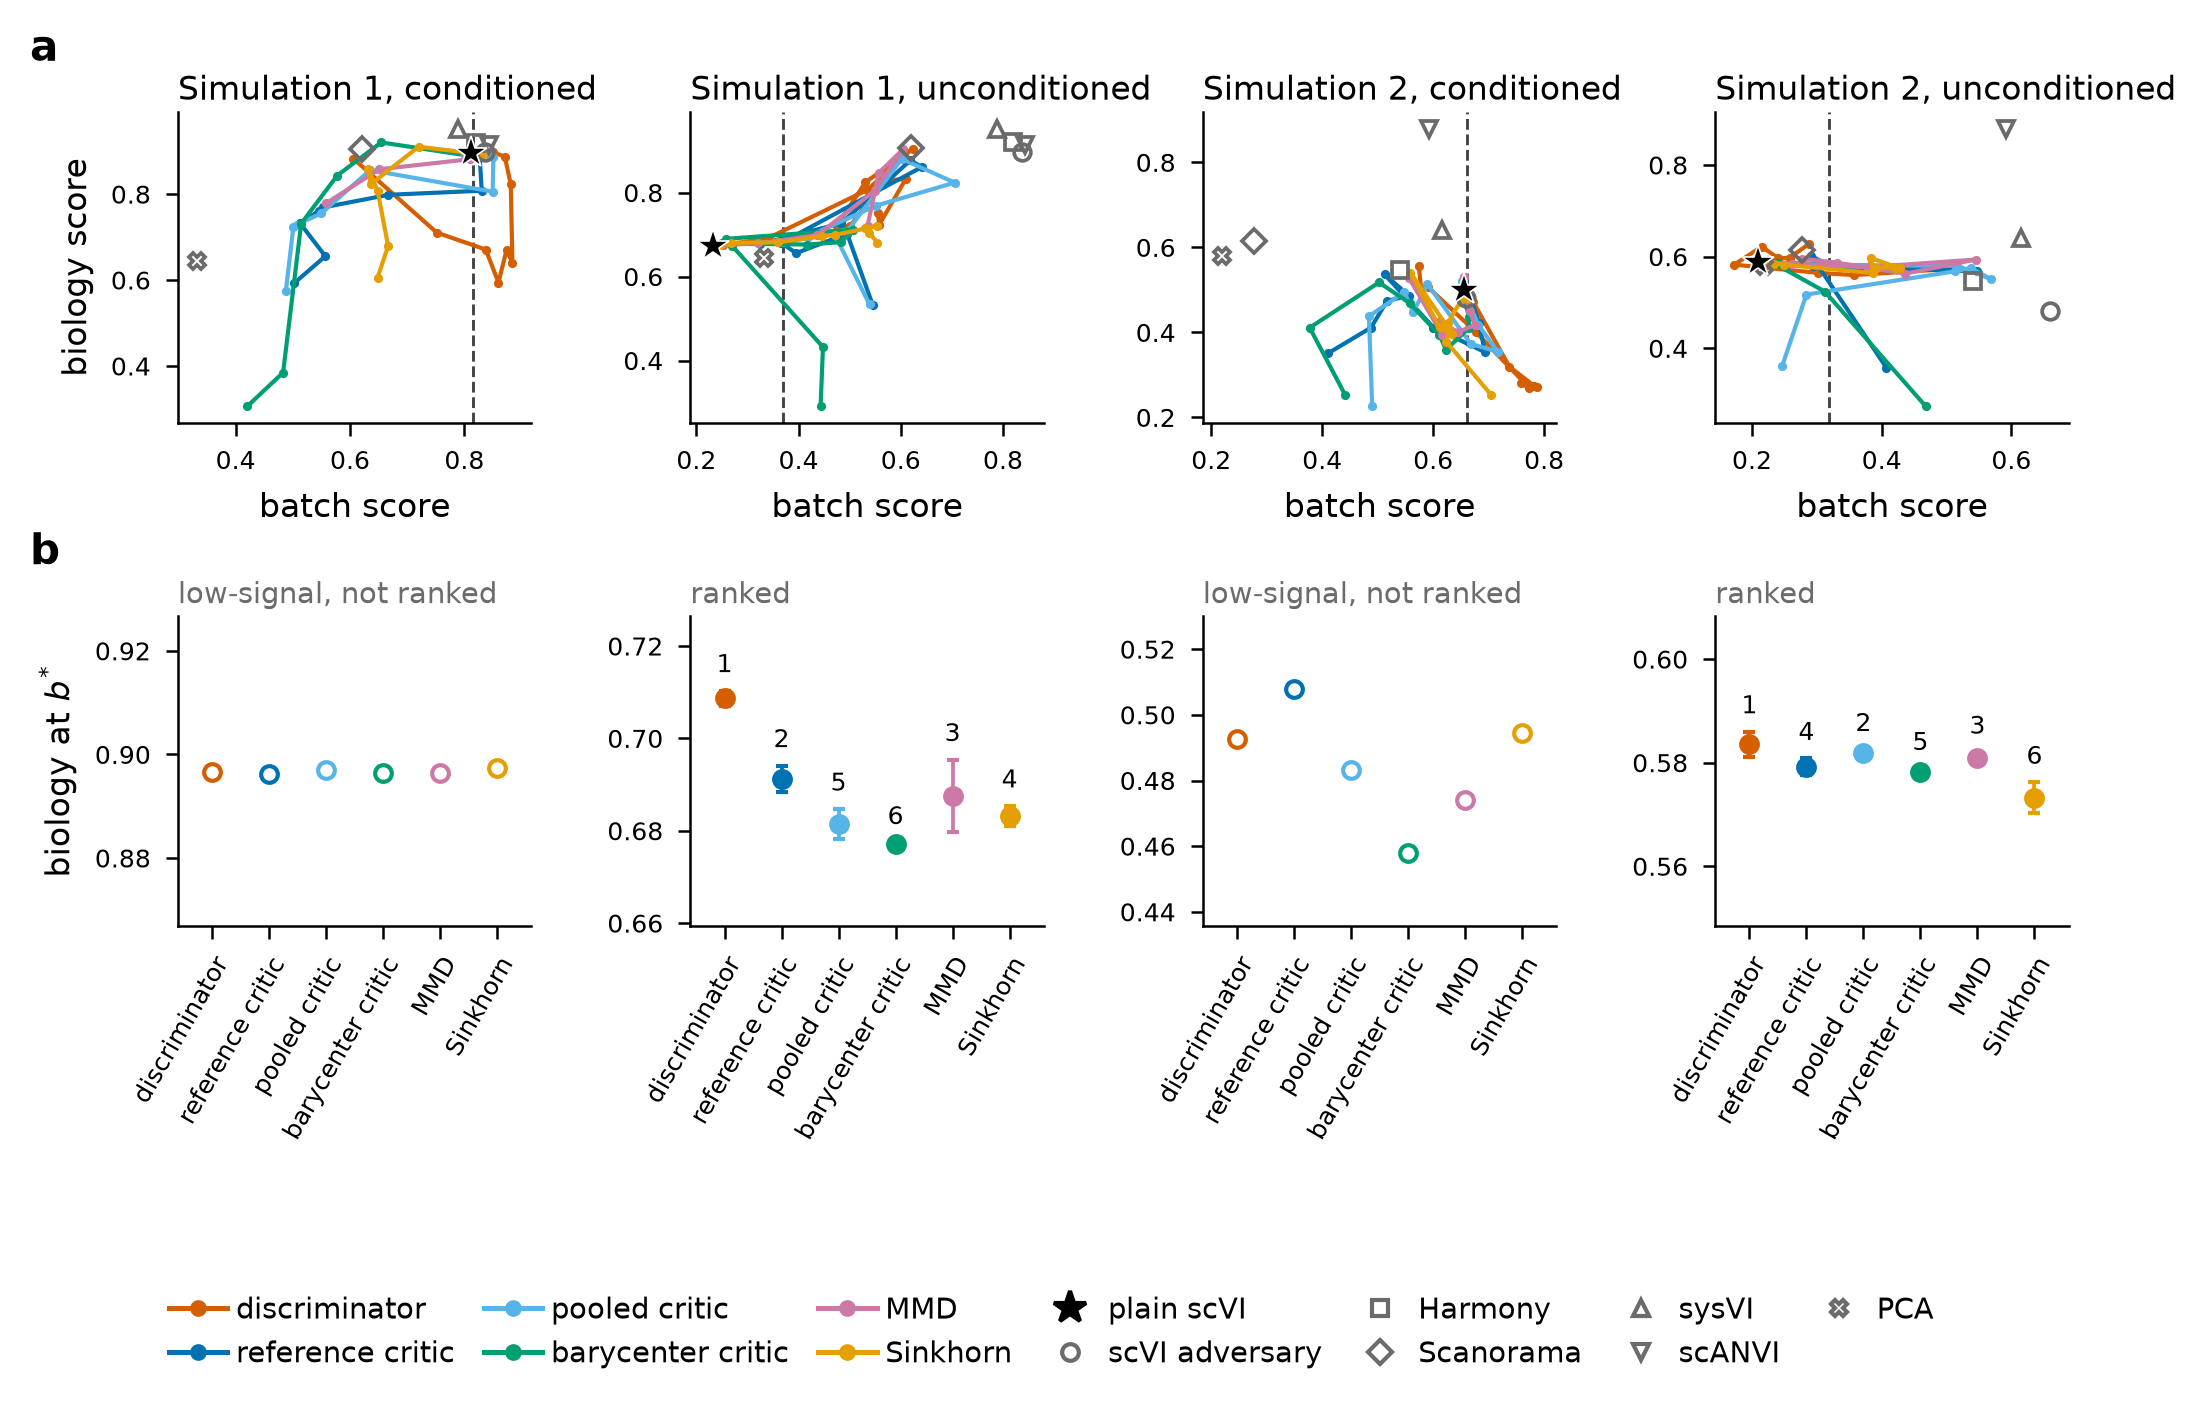
\includegraphics[width=\textwidth]{figures/figS1.png}
\caption{Simulation tasks with both decoders. \textbf{(a)} Seed-mean batch and biology scores across strengths, with plain scVI as a star, $b^*$ dashed and each standard tool's best selection-score setting in grey. \textbf{(b)} Biology at $b^*$ with leave-one-seed-out errors and ranks. Open markers identify low-signal batch-conditioned simulations, shown without errors or ranks. Simulations are ranked separately from real tasks (Supplementary Notes 5 and 6).}\label{fig:s1}
\end{figure}

\begin{figure}[p]
\centering\renewcommand{\figurename}{Supplementary Figure}\renewcommand{\thefigure}{S2}%
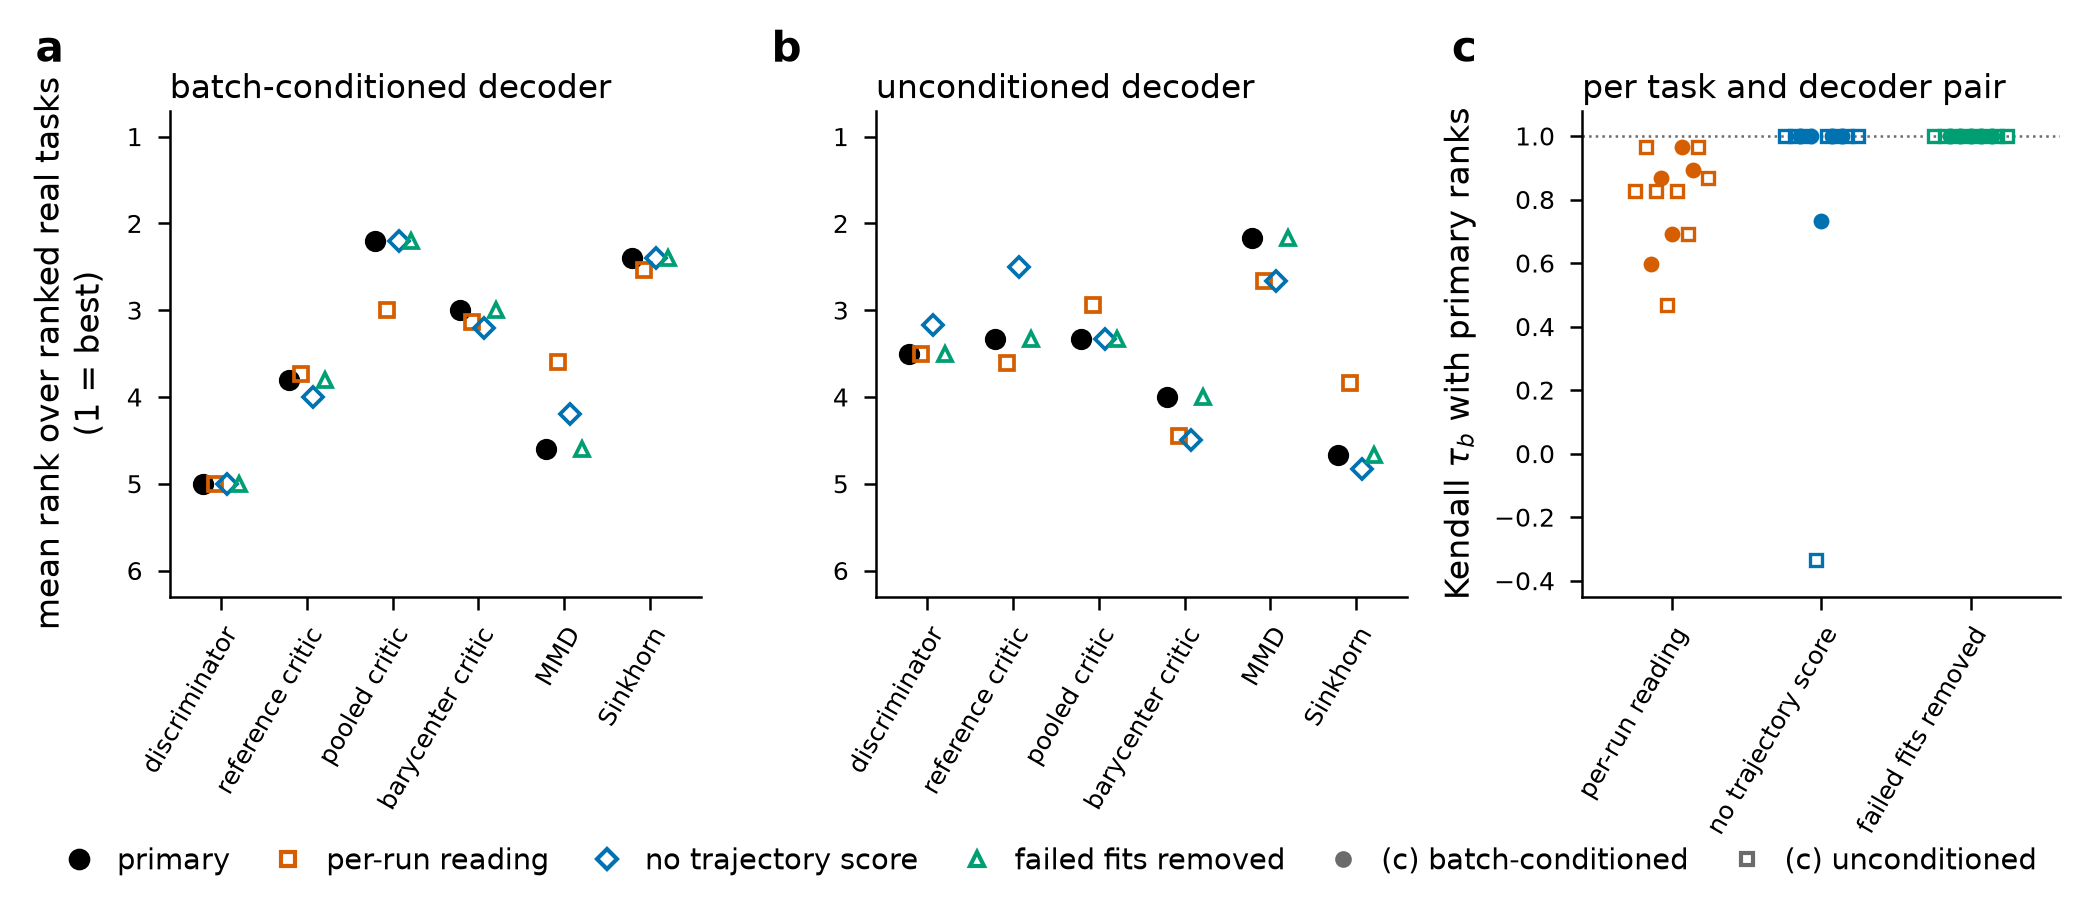
\includegraphics[width=\textwidth]{figures/figS2.png}
\caption{Sensitivity of rankings to per-seed readings, omission of trajectory conservation and removal of strengths containing failed fits. The last reproduces primary ranks because no fit failed. \textbf{(a, b)} Mean ranks across ranked real tasks by decoder. \textbf{(c)} Kendall's $\tau_b$ against primary ranks in each of 13 ranked pairs, including simulations. Points at 1 overlap (Supplementary Note 6).}\label{fig:s2}
\end{figure}

\begin{figure}[p]
\centering\renewcommand{\figurename}{Supplementary Figure}\renewcommand{\thefigure}{S3}%
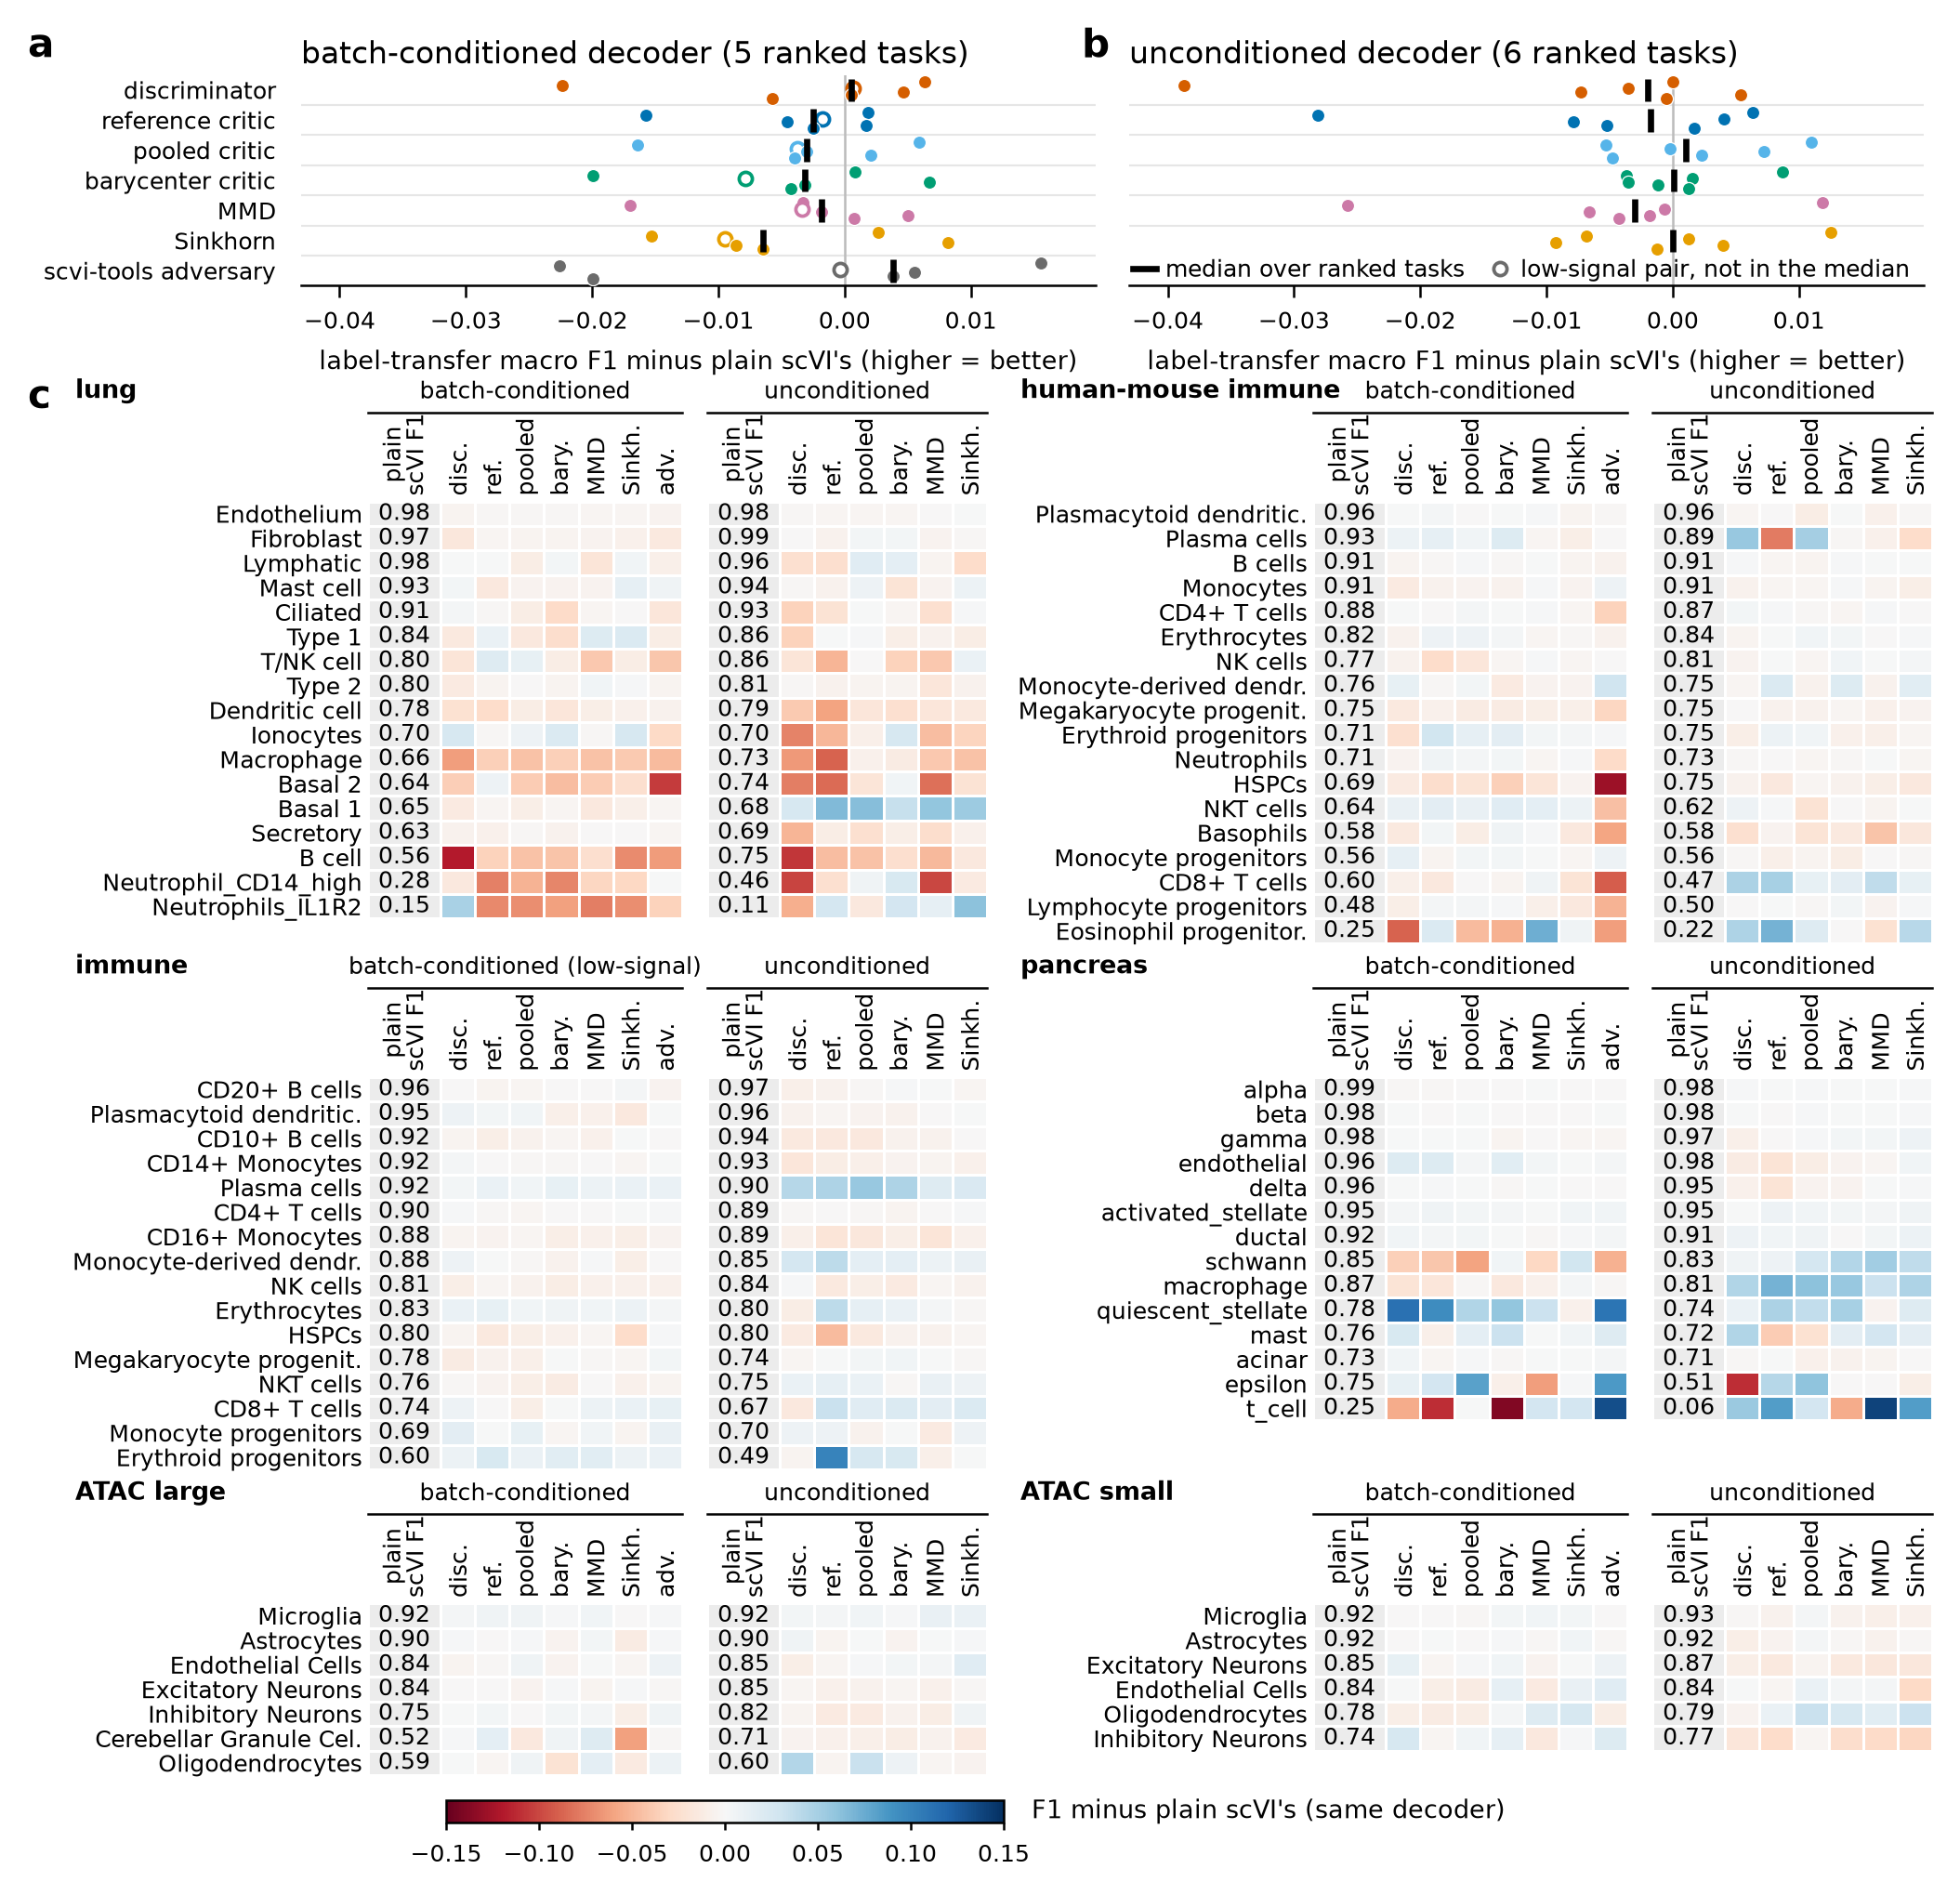
\includegraphics[width=\textwidth,height=0.76\textheight,keepaspectratio]{figures/figS3.png}
\caption{Label transfer at first-crossing strengths on real tasks (Supplementary Note 9). Plain scVI and the scvi-tools adversary are unmatched. \textbf{(a, b)} Macro-F1 differences from same-decoder plain scVI for batch-conditioned and unconditioned models. Dots are tasks; black ticks are ranked-task medians. The open immune dot is low-signal and excluded from its median. \textbf{(c)} Per-type F1 averaged over held-out batches and seeds. Grey shows plain scVI; colours show differences, blue above and red below, limited to $\pm0.15$. Types are ordered by plain-scVI F1. Abbreviations denote discriminator, reference critic, barycenter critic, Sinkhorn divergence and scvi-tools adversary.}\label{fig:s3}
\end{figure}

\begin{figure}[p]
\centering\renewcommand{\figurename}{Supplementary Figure}\renewcommand{\thefigure}{S4a}%
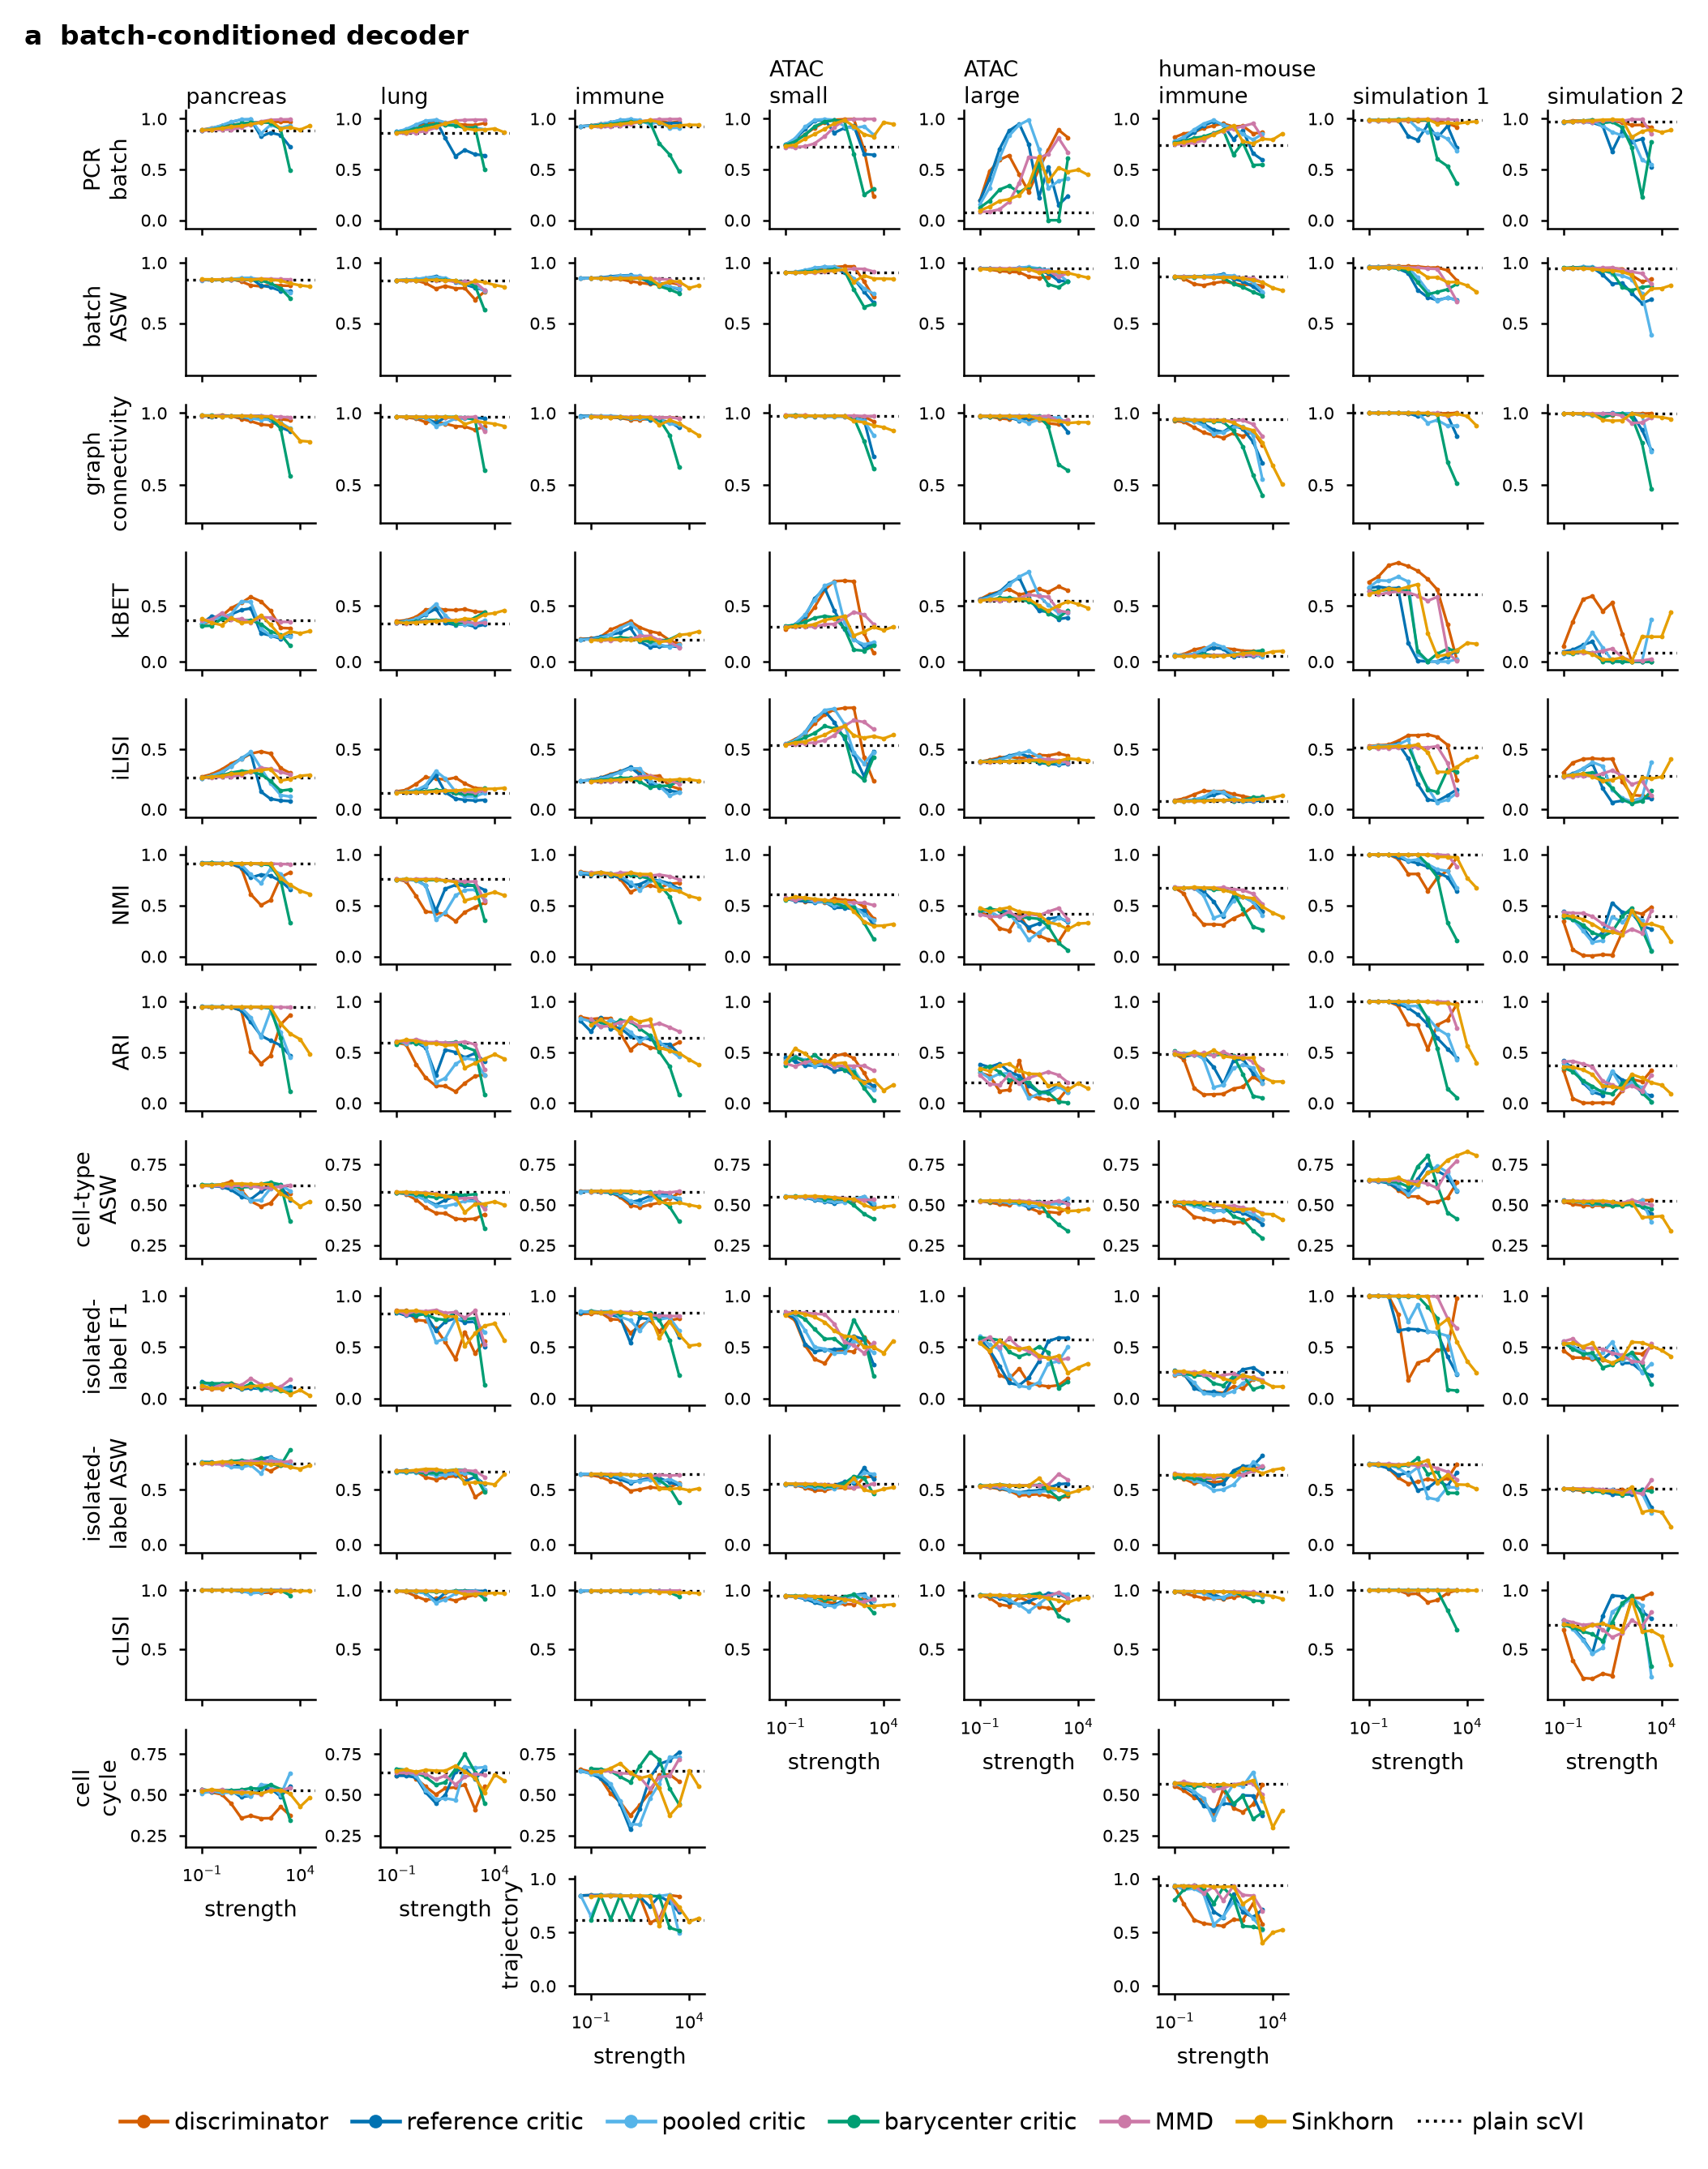
\includegraphics[width=\textwidth,height=0.78\textheight,keepaspectratio]{figures/figS4a.png}
\caption{Individual metric curves with the batch-conditioned decoder. Rows show unscaled batch metrics (1--5) and biology metrics (6--13); columns show tasks. Lines join means over three seeds against log penalty strength. Dotted lines denote plain scVI. Each row shares a vertical scale. Cell-cycle conservation applies to the four real RNA tasks and trajectory conservation to both immune tasks; other panels are empty (Supplementary Note 3).}\label{fig:s4a}
\end{figure}

\begin{figure}[p]
\centering\renewcommand{\figurename}{Supplementary Figure}\renewcommand{\thefigure}{S4b}%
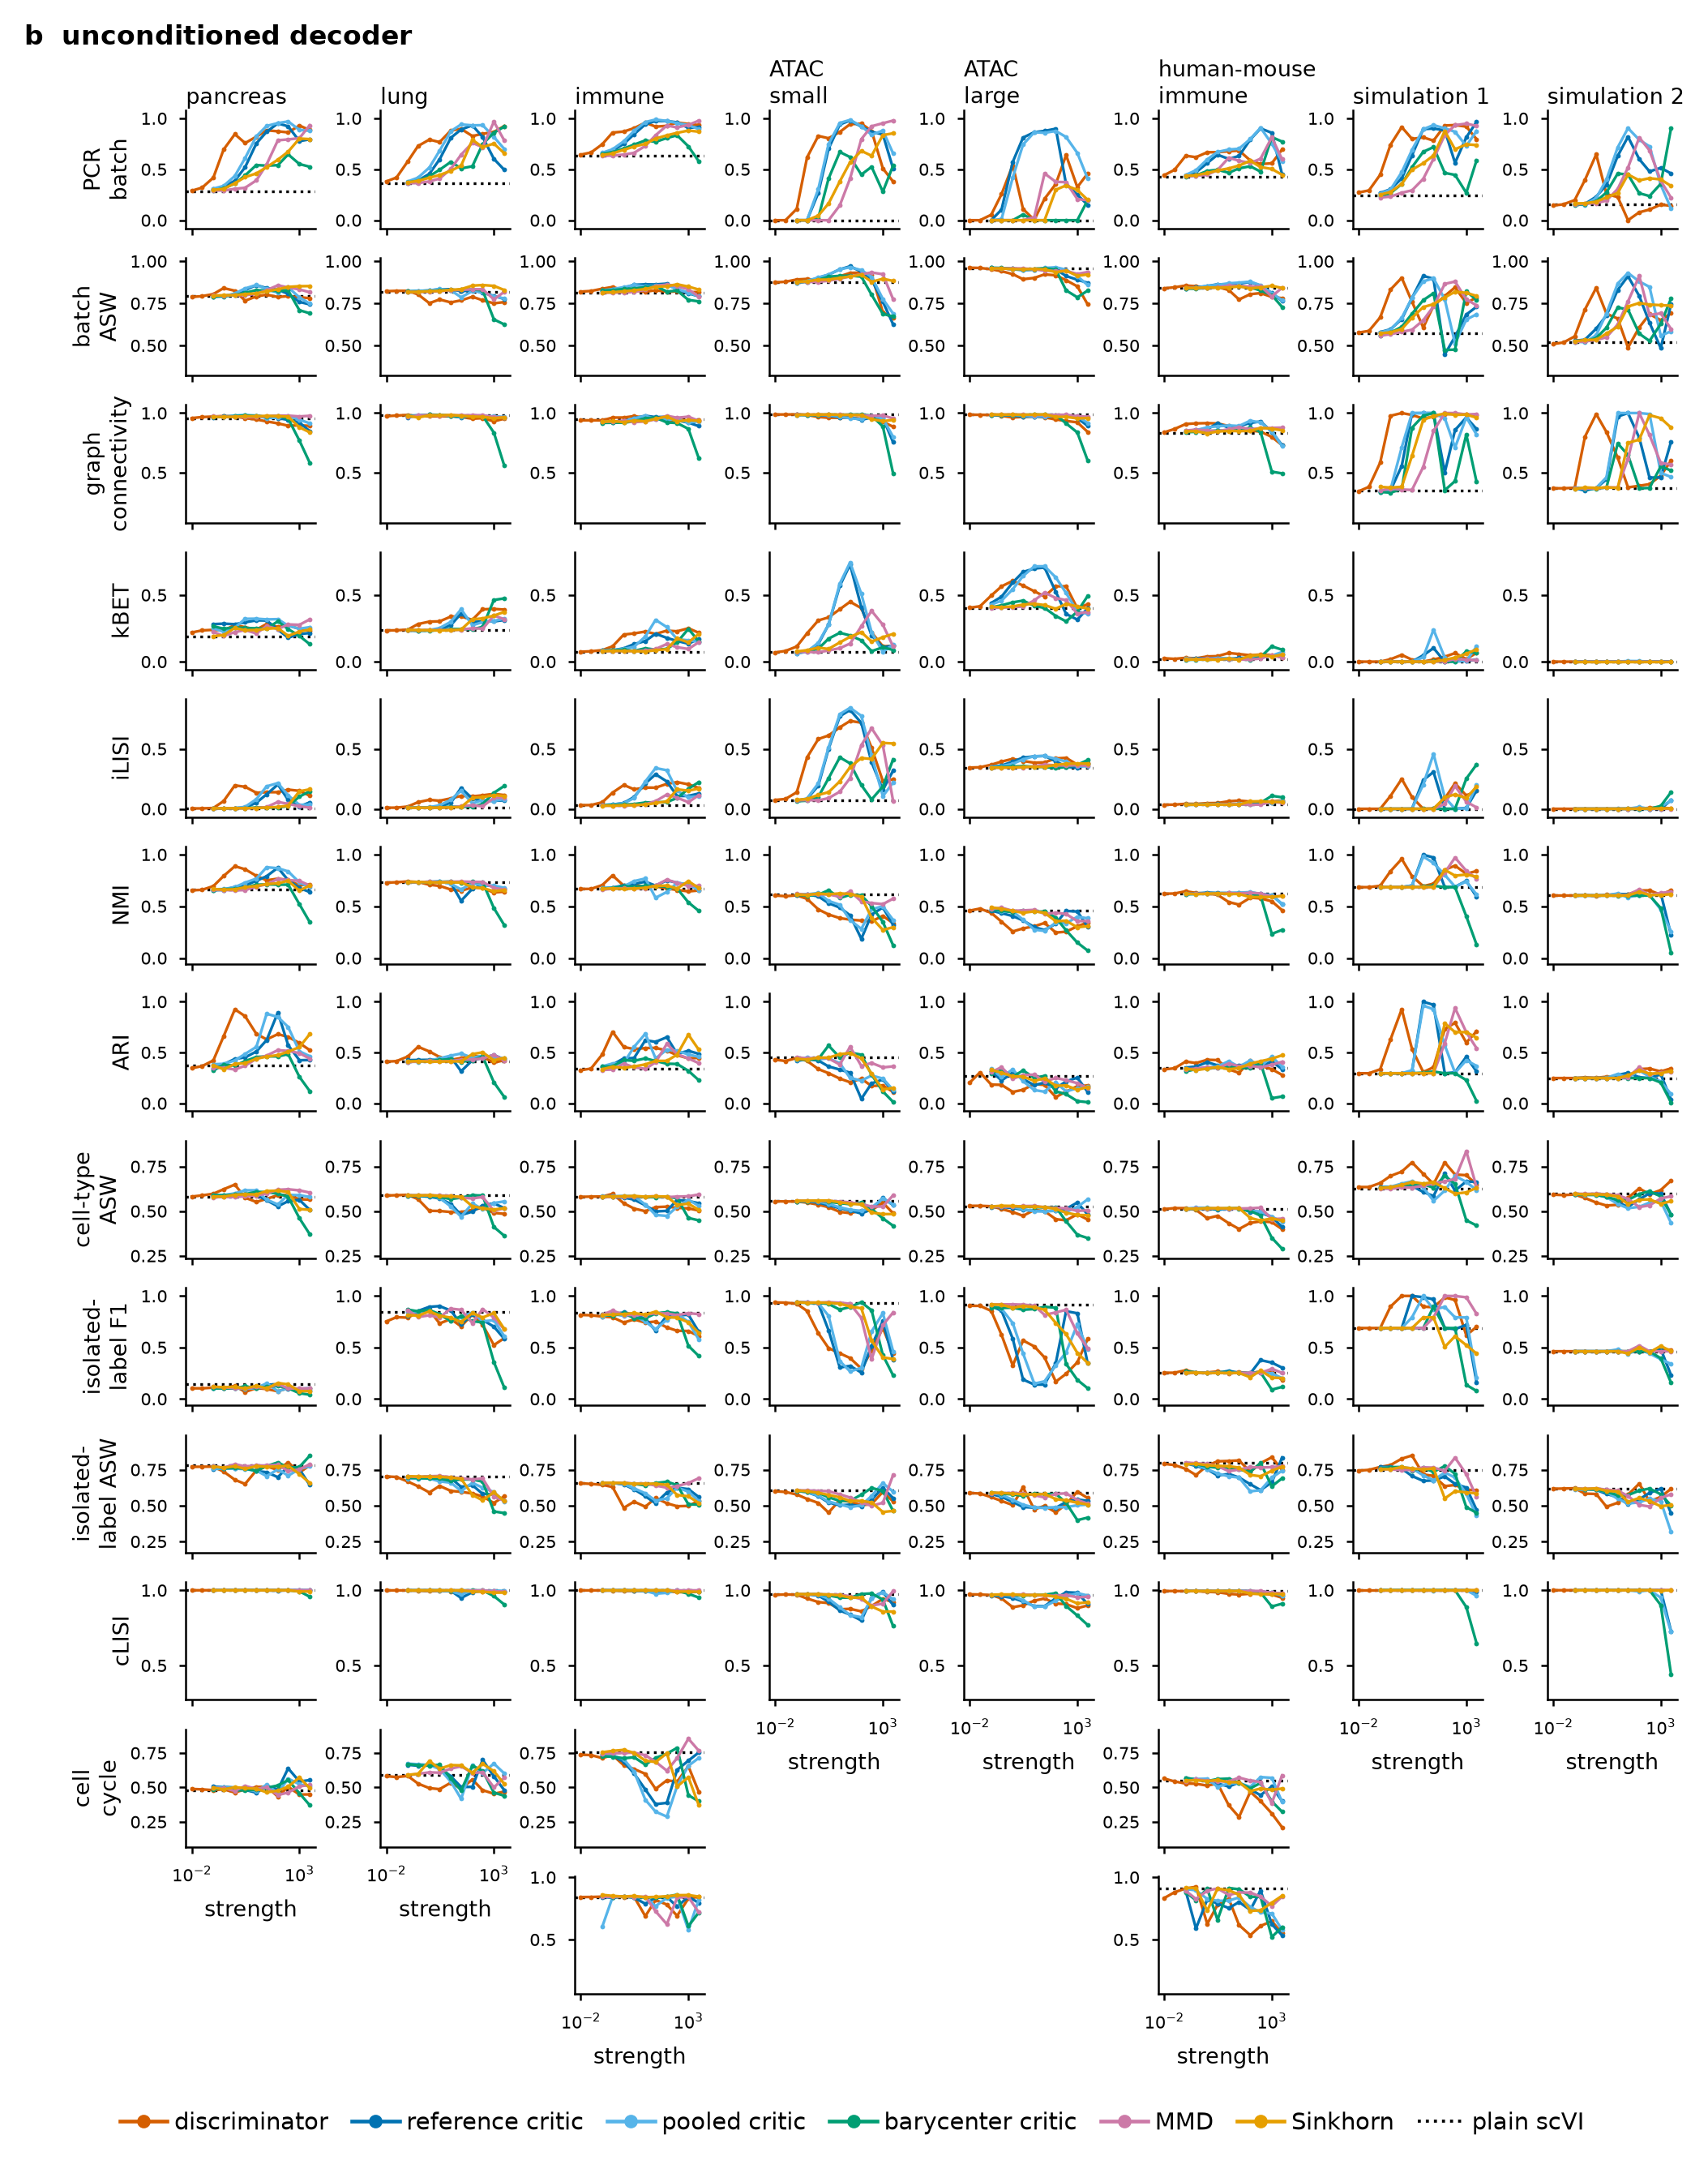
\includegraphics[width=\textwidth,height=0.78\textheight,keepaspectratio]{figures/figS4b.png}
\caption{Individual metric curves with the unconditioned decoder. Layout and definitions follow Supplementary Figure S4a.}\label{fig:s4b}
\end{figure}

\begin{figure}[p]
\centering\renewcommand{\figurename}{Supplementary Figure}\renewcommand{\thefigure}{S5}%
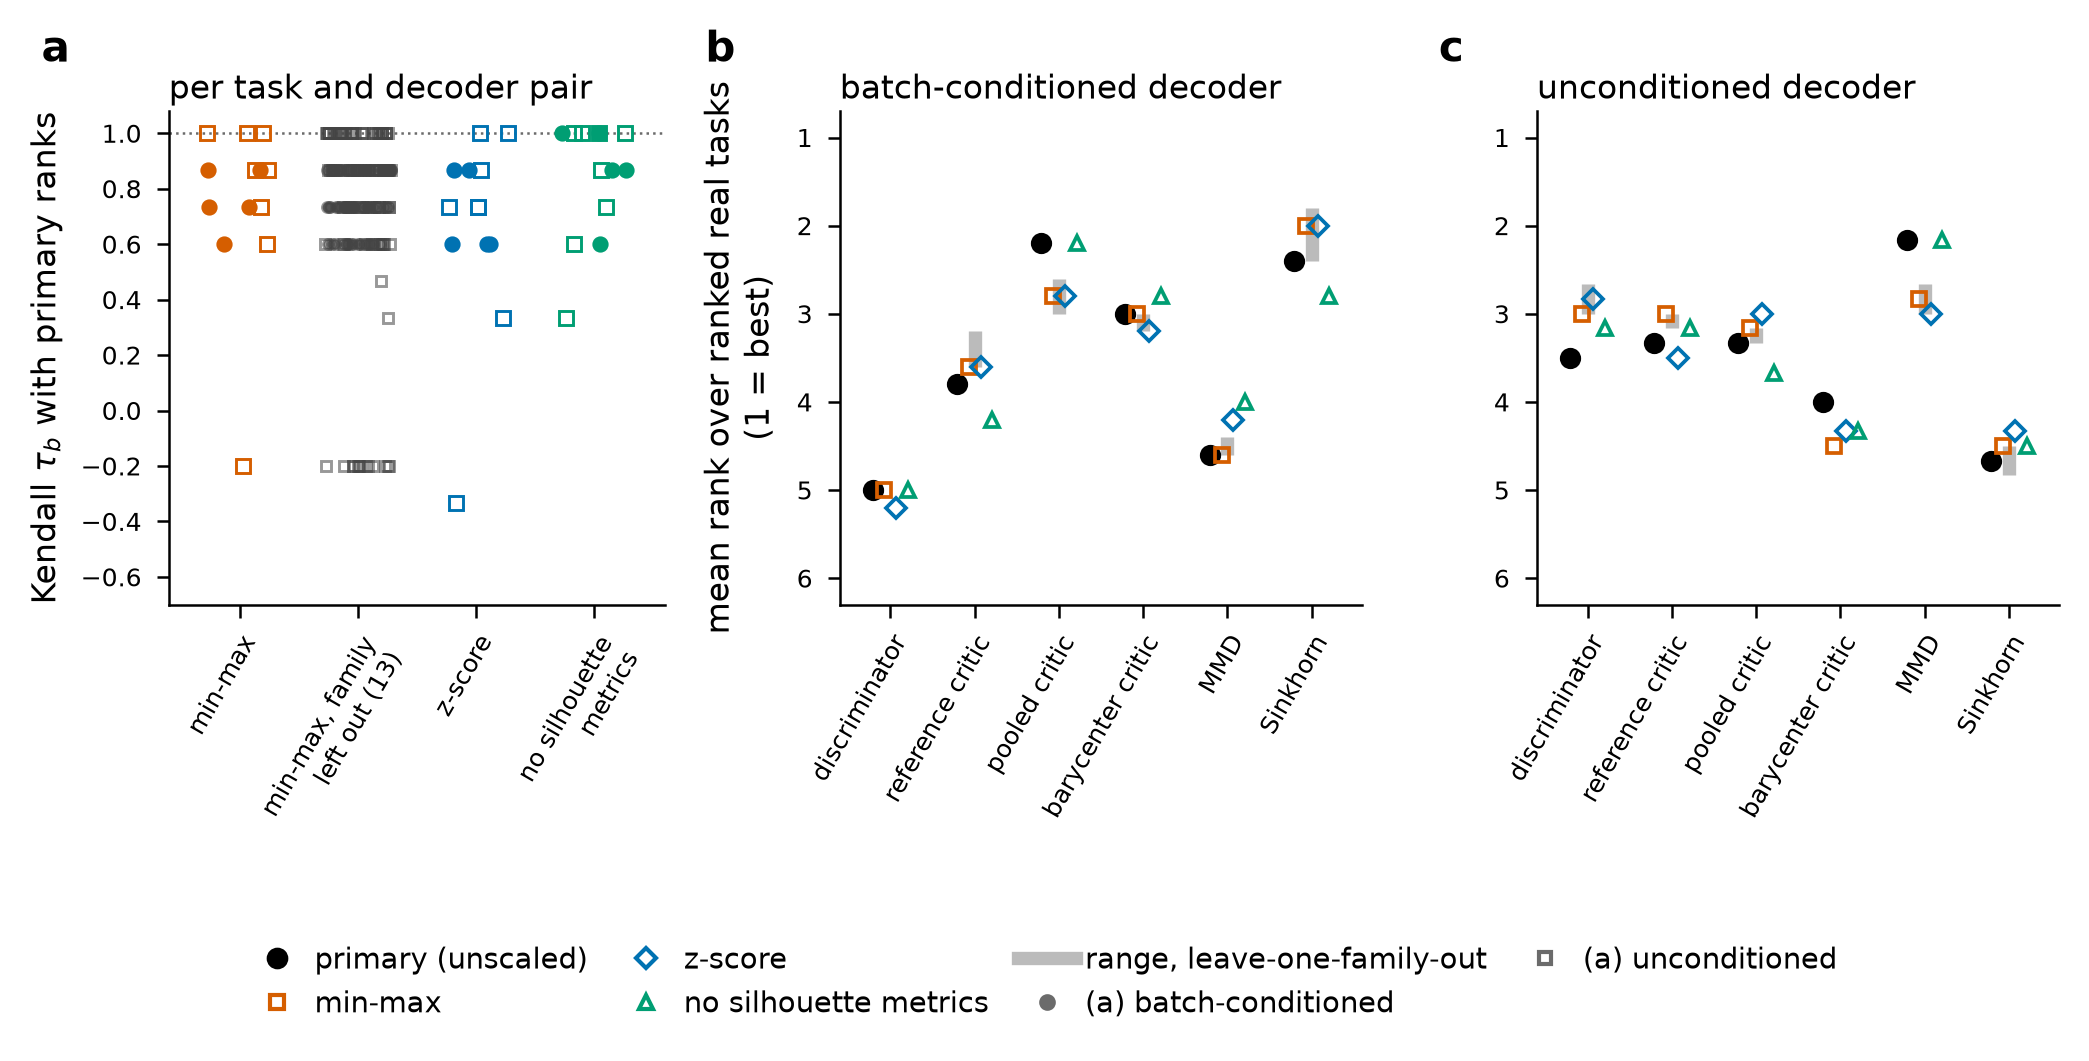
\includegraphics[width=\textwidth]{figures/figS5.png}
\caption{Sensitivity to metric scaling and composition (Supplementary Note 6). Variants use min--max scaling, omission of each method family from its scaling reference, z-scores, or exclusion of the three silhouette metrics. Scores, $b^*$ and ranks are recomputed. \textbf{(a)} Kendall's $\tau_b$ against primary rankings, with points for each ranked pair and, where applicable, omitted family. \textbf{(b, c)} Mean ranks across ranked real tasks by decoder. Grey bars span the 13 family-omission runs. Scaling can change the leading penalty.}\label{fig:s5}
\end{figure}

\begin{figure}[p]
\centering\renewcommand{\figurename}{Supplementary Figure}\renewcommand{\thefigure}{S6}%
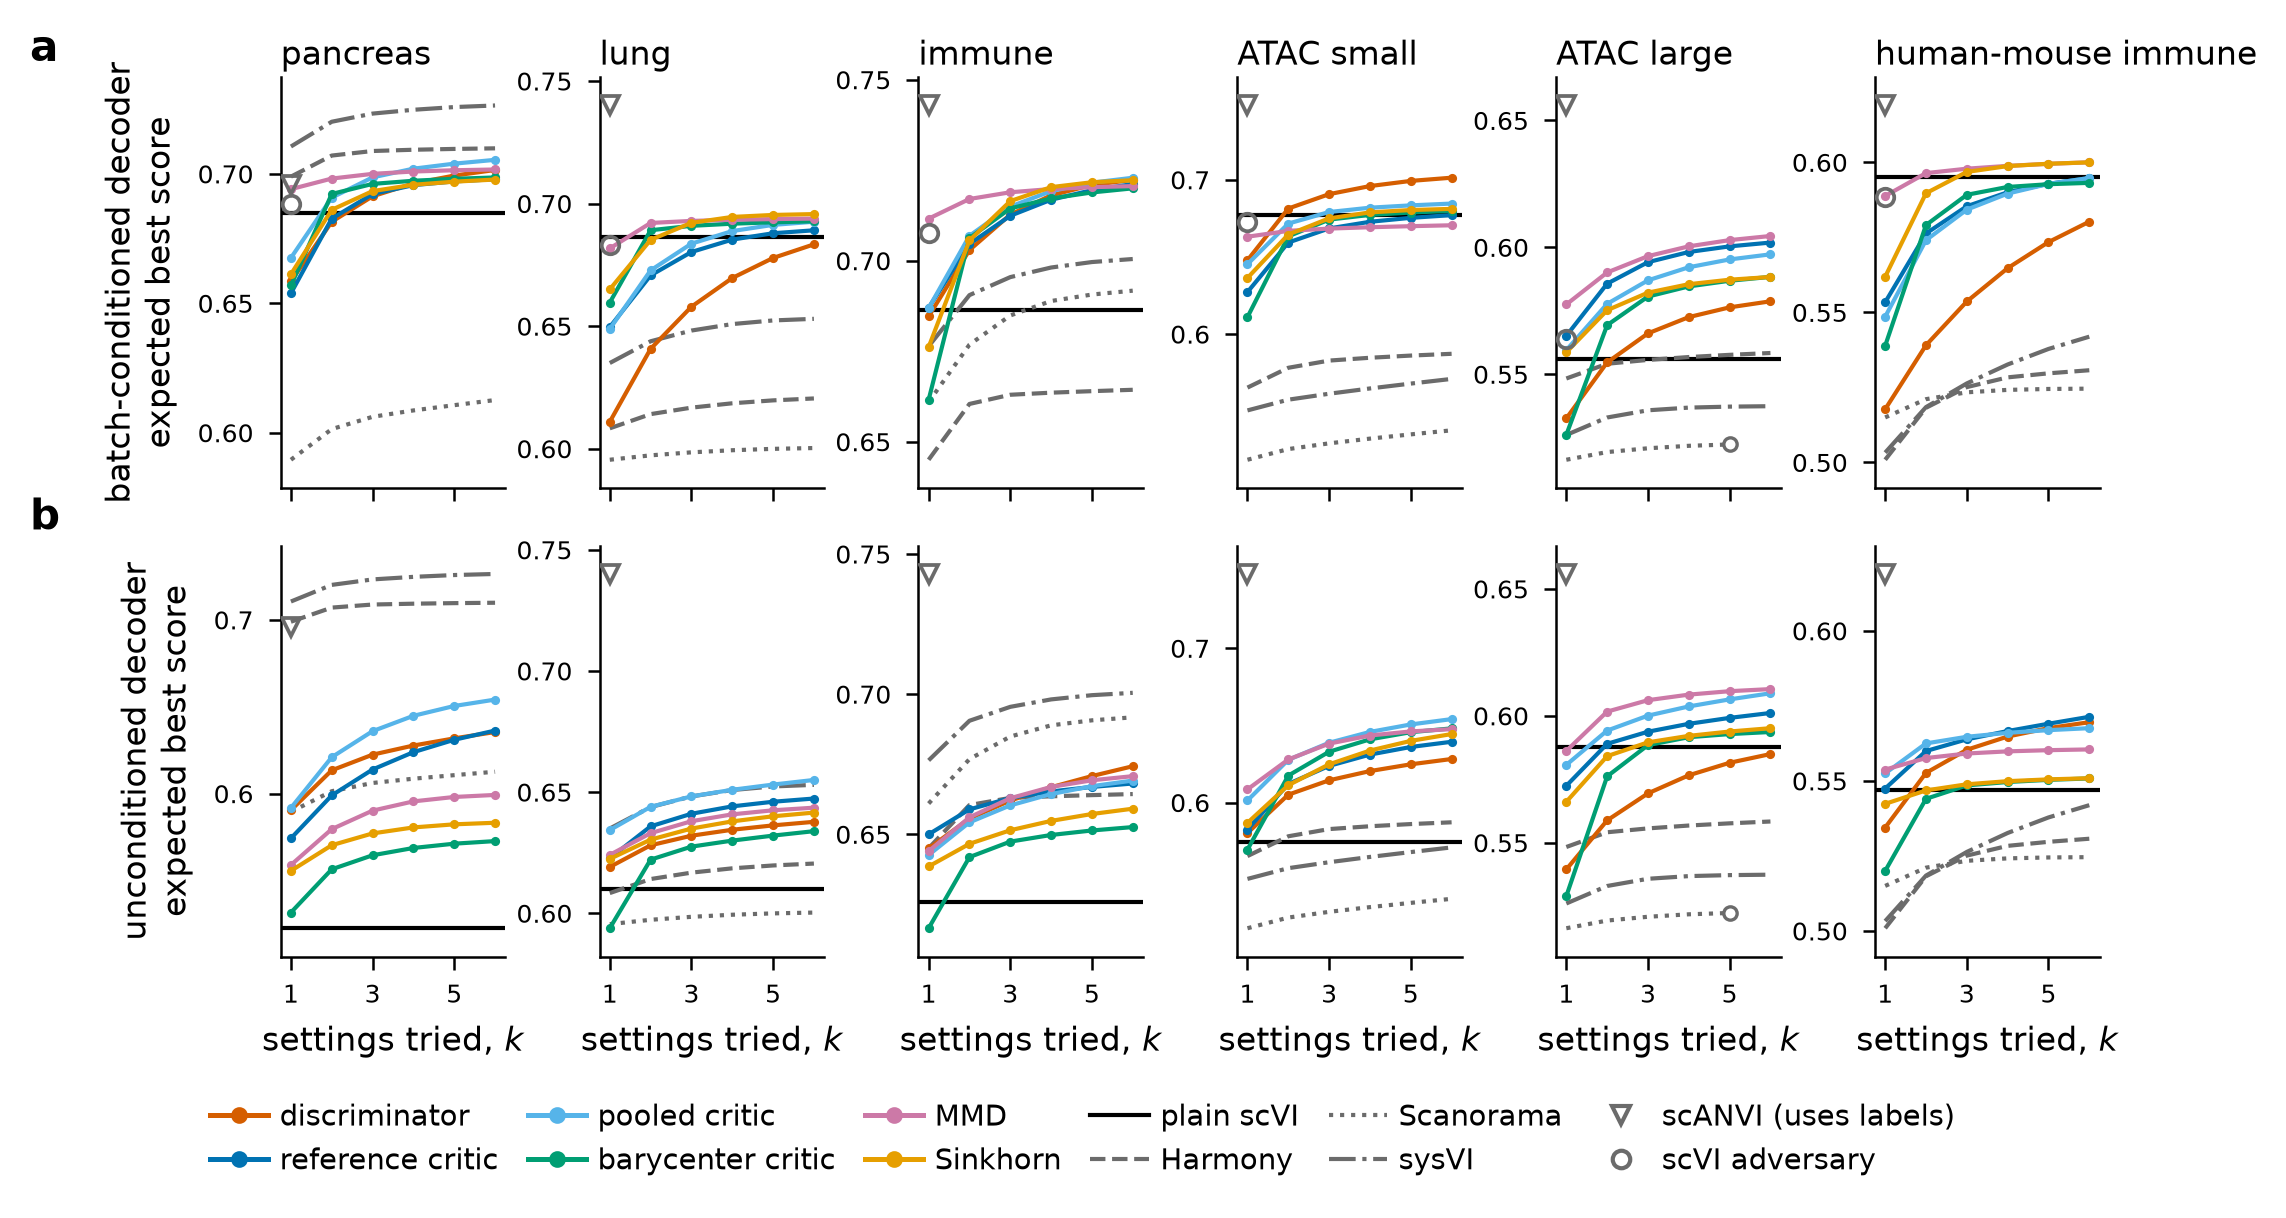
\includegraphics[width=\textwidth]{figures/figS6.png}
\caption{Trade-off curves for six real tasks with batch-conditioned \textbf{(a)} and unconditioned \textbf{(b)} decoders. Lines join seed-mean scores from plain scVI (star) through increasing penalty strengths. Open circles mark strongest settings; dashed lines mark $b^*$. Grey identifies the low-signal immune pair. Panels within columns share axes. Supplementary Figure S7 compares biology at $b^*$ and at the strongest setting.}\label{fig:s6}
\end{figure}

\begin{figure}[p]
\centering\renewcommand{\figurename}{Supplementary Figure}\renewcommand{\thefigure}{S7}%
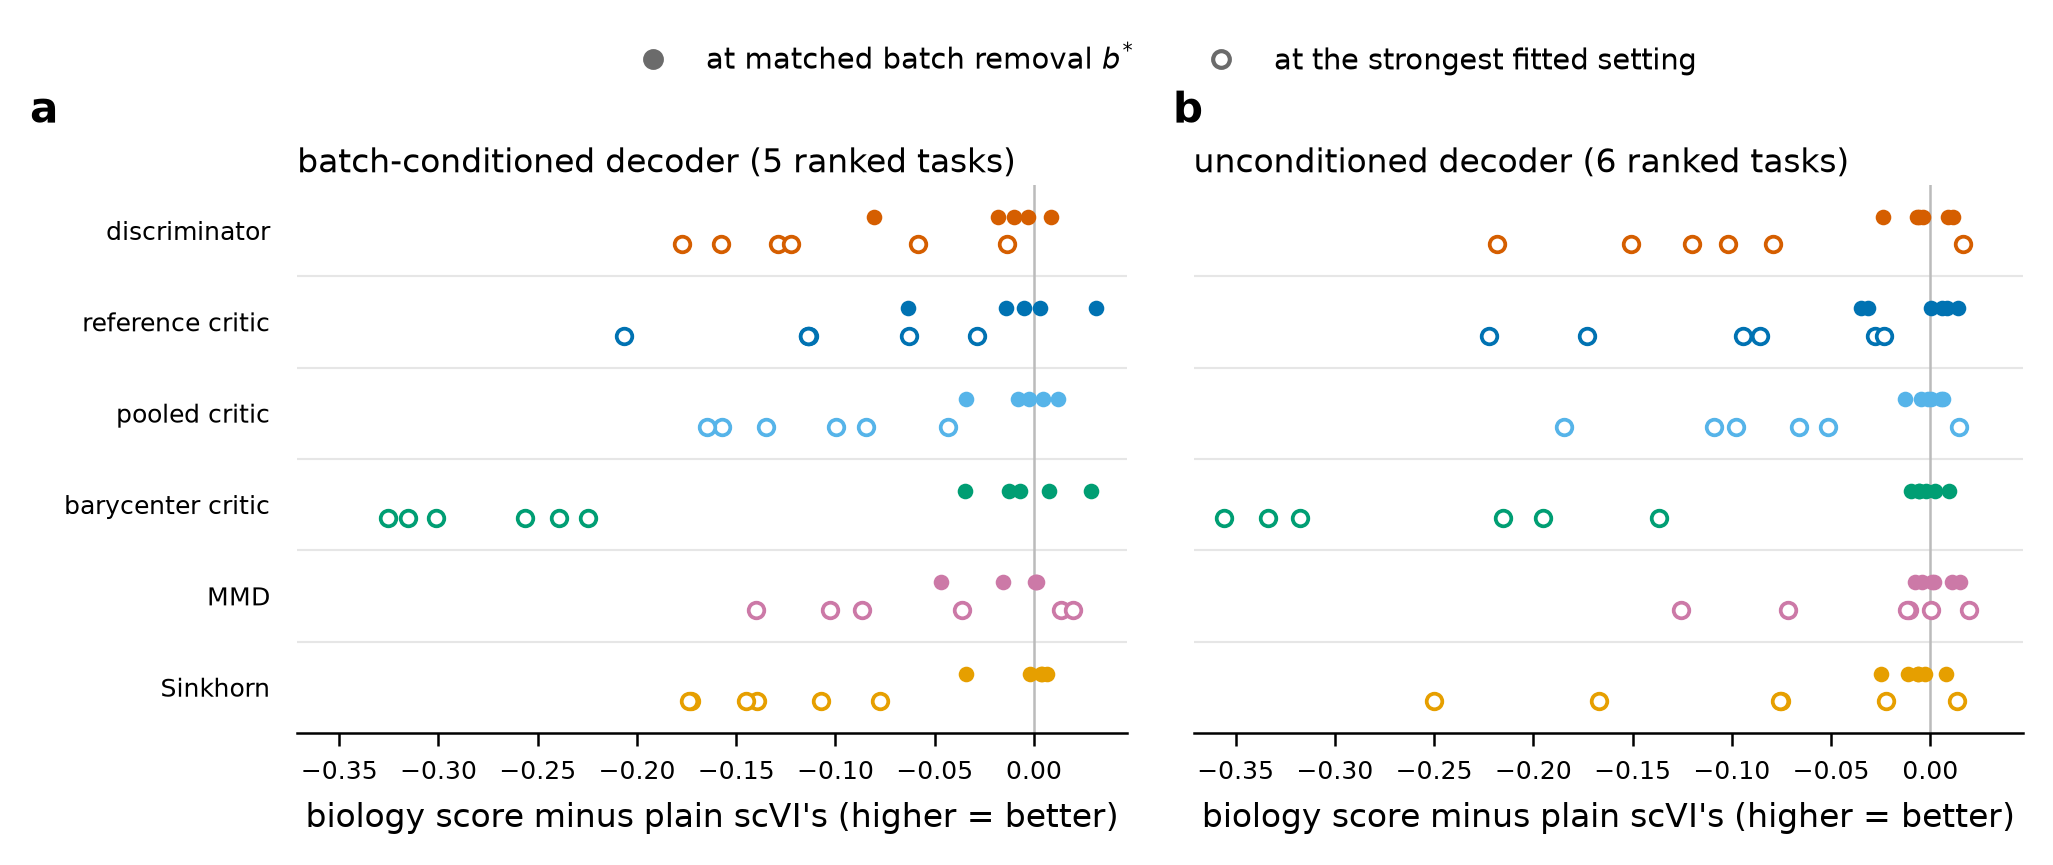
\includegraphics[width=\textwidth]{figures/figS7.png}
\caption{Biology differences from same-decoder plain scVI at $b^*$ (filled dots) and the strongest fitted setting (open dots). Panels show batch-conditioned \textbf{(a)} and unconditioned \textbf{(b)} decoders. Each dot represents a real task; grey marks no change. Filled dots exclude the low-signal immune pair, while open dots include all tasks. Supplementary Figure S6 gives full curves.}\label{fig:s7}
\end{figure}

\begin{figure}[p]
\centering\renewcommand{\figurename}{Supplementary Figure}\renewcommand{\thefigure}{S8}%
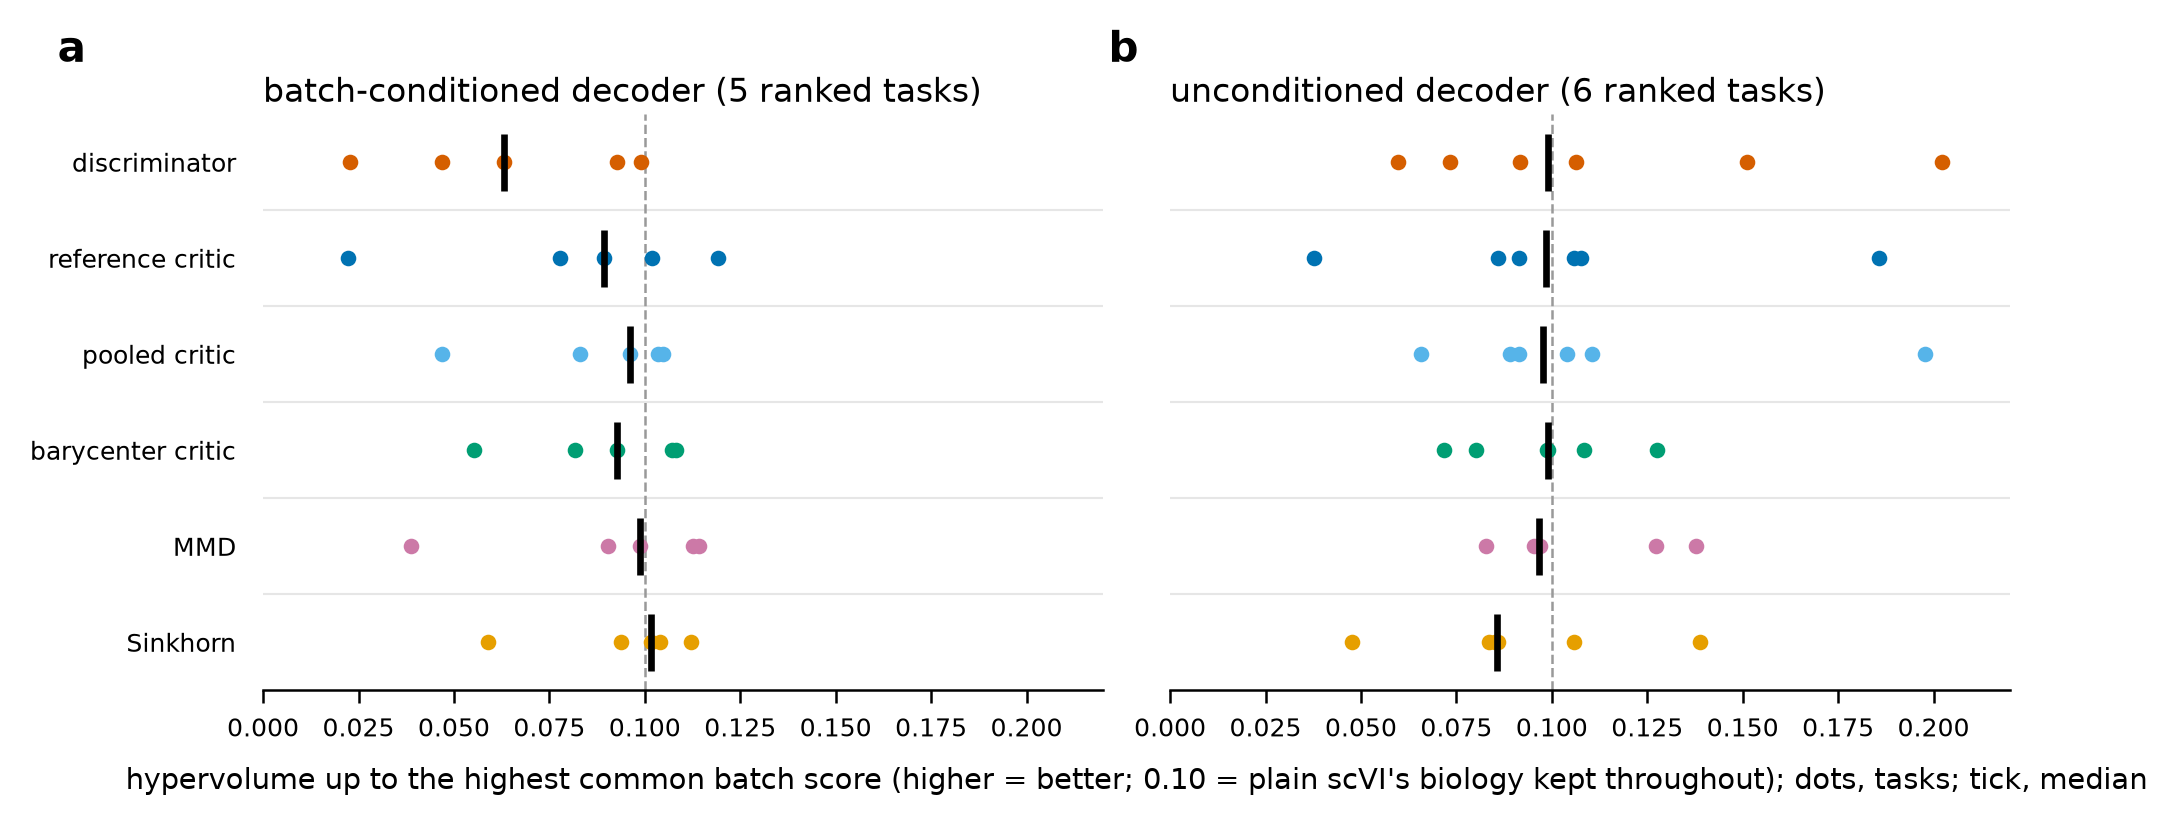
\includegraphics[width=\textwidth]{figures/figS8.png}
\caption{Hypervolume capped at the highest common batch score, with batch-conditioned \textbf{(a)} and unconditioned \textbf{(b)} decoders. Dots represent ranked real tasks and black ticks their median. The area lies under each Pareto frontier above biology difference $-0.10$, divided by the common batch gap. The dashed value 0.10 denotes retention of plain-scVI biology throughout. Supplementary Note 7 defines the measure; Supplementary Table S8 also gives uncapped values.}\label{fig:s8}
\end{figure}

\begin{figure}[p]
\centering\renewcommand{\figurename}{Supplementary Figure}\renewcommand{\thefigure}{S9}%
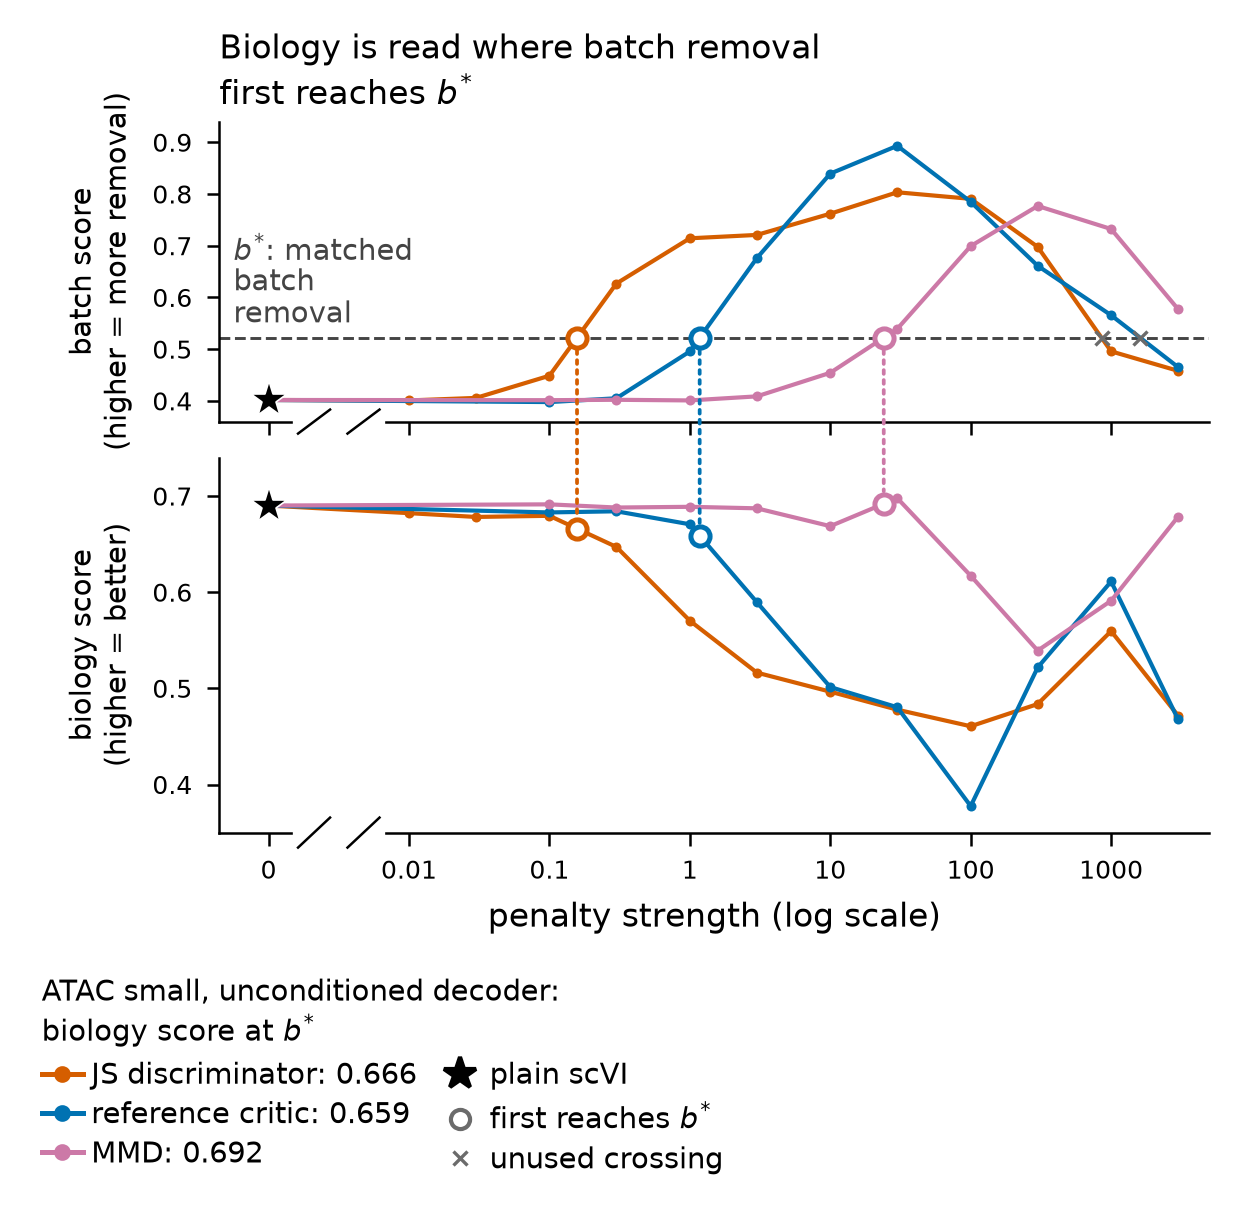
\includegraphics[width=0.6\textwidth]{figures/figS9.png}
\caption{Reading biology at $b^*$ on unconditioned ATAC small for the discriminator, reference critic and MMD. Curves show mean scores over seeds 100--102 against log strength, with plain scVI at 0 beyond the axis break. Open circles bracket the first crossing of dashed $b^*$; dotted segments show interpolation in batch score. Later crossings, marked by grey crosses, are ignored. The legend gives biology at $b^*$ (Supplementary Note 5).}\label{fig:s9}
\end{figure}


\end{document}
